% ============================================================
% Rapport de PFE — Credit Risk Intelligence Platform
% Compilation : pdfLaTeX, puis biber pour la bibliographie
%   (séquence Overleaf/latexmk standard : pdflatex -> biber -> pdflatex -> pdflatex)
% ============================================================

\documentclass[12pt]{report}

% ---------- Mise en page ----------
\usepackage[a4paper,margin=2.5cm]{geometry}
\usepackage[T1]{fontenc}
\usepackage[utf8]{inputenc}
\usepackage[french]{babel}
\usepackage{mathptmx}          % police façon Times New Roman
\usepackage{setspace}
\setstretch{1.15}              % interligne 1,15
\usepackage{csquotes}          % guillemets français via \enquote{...}

% ---------- Paragraphes ----------
\setlength{\parindent}{0.5cm}  % alinéa de première ligne
\setlength{\parskip}{0pt}

% ---------- Figures, tableaux ----------
\usepackage{graphicx}
\usepackage{booktabs}
\usepackage{caption}
\usepackage{float}
\usepackage{tikz}
\usetikzlibrary{arrows.meta, positioning}
\usepackage{svg}              % logos technologiques (chapitre 6) — rendu via Inkscape sur Overleaf
\usepackage{tcolorbox}
\tcbuselibrary{skins,raster}

% ---------- Titres hiérarchisés (tailles décroissantes) ----------
\usepackage{titlesec}
\titleformat{\chapter}[display]{\normalfont\huge\bfseries}{\chaptertitlename\ \thechapter}{20pt}{\Huge}
\titleformat{\section}{\normalfont\Large\bfseries}{\thesection}{1em}{}
\titleformat{\subsection}{\normalfont\large\bfseries}{\thesubsection}{1em}{}
\titleformat{\subsubsection}{\normalfont\normalsize\bfseries}{\thesubsubsection}{1em}{}

% ---------- Pagination "page / total", en bas à droite ----------
\usepackage{fancyhdr}
\usepackage{lastpage}
\pagestyle{fancy}
\fancyhf{}
\renewcommand{\headrulewidth}{0pt}
\fancyfoot[R]{\thepage\ / \pageref{LastPage}}

% ---------- Bibliographie ----------
\usepackage[backend=biber,style=authoryear,sorting=nyt]{biblatex}
\addbibresource{biblio.bib}

% ---------- Références croisées ----------
\usepackage[hidelinks]{hyperref}

% ---------- Cartes technologiques (chapitre 6) ----------
\tcbset{
  techcard/.style={
    colback=white, colframe=black!35, boxrule=0.4pt,
    arc=2mm, width=4.3cm, height=5.4cm,
    valign=top, halign=center, boxsep=2pt, left=3pt, right=3pt, top=6pt, bottom=4pt,
  }
}
\newcommand{\techcard}[4]{%
  \begin{tcolorbox}[techcard]
    \includesvg[height=1cm]{#1}\\[5pt]
    {\bfseries #2}\\[2pt]
    {\footnotesize\itshape #3}\\[5pt]
    {\footnotesize #4}
  \end{tcolorbox}%
}
% Variante sans logo — aucune icône de marque officielle disponible
% pour cet outil (vérifié), jamais un logo approximatif substitué.
\newcommand{\techcardtext}[3]{%
  \begin{tcolorbox}[techcard]
    \rule{0pt}{1cm}\\[5pt]
    {\bfseries #1}\\[2pt]
    {\footnotesize\itshape #2}\\[5pt]
    {\footnotesize #3}
  \end{tcolorbox}%
}

\begin{document}

% ============================================================
% Page de garde — modèle officiel fourni (ESPRIT / EY Tunisie)
% ============================================================
\begin{titlepage}
\newgeometry{margin=0cm}
\thispagestyle{empty}
\centering

\includegraphics[width=\paperwidth,height=\paperheight]{figures/page_de_garde.png}
\restoregeometry
\end{titlepage}


\pagenumbering{roman}
\tableofcontents
\clearpage
\pagenumbering{arabic}
\setcounter{page}{1}

\chapter*{Introduction générale}
\addcontentsline{toc}{chapter}{Introduction générale}

Le crédit occupe une place centrale dans le financement de l'activité économique. En accordant un prêt, une banque ne se contente pas de mettre des fonds à la disposition d'un client : elle engage ses propres ressources sur la base d'une appréciation du risque que ce client ne puisse, en tout ou en partie, honorer ses engagements. Cette appréciation conditionne directement la solidité financière de l'établissement : un risque mal maîtrisé peut se traduire par des pertes, tandis qu'une prudence excessive prive la banque de financements par ailleurs rentables. La gestion du crédit repose ainsi sur un équilibre permanent entre plusieurs préoccupations difficiles à concilier : limiter le risque de défaut, anticiper les pertes qu'il peut engendrer, et disposer de fonds propres suffisants pour absorber les pertes inattendues.

C'est dans ce contexte que s'inscrit le projet de fin d'études présenté dans ce rapport, consacré à la gestion du risque de crédit bancaire et réalisé au sein de l'entité AI~\&~Data d'EY~Tunisie. Ce rapport constitue également le mémoire de stage de fin d'études du Master Actuariat, dont il valide la dernière étape académique. Ce domaine nécessite de faire converger l'évaluation quantitative du risque et la compréhension du fonctionnement réel d'une banque afin de concevoir des outils utiles à la décision. Le projet porte ainsi sur plusieurs dimensions complémentaires : le risque de crédit associé à chaque client, les pertes attendues, le capital nécessaire pour absorber les pertes inattendues et la rentabilité du financement accordé. Leur prise en compte constitue le fil conducteur de ce rapport. La problématique à laquelle répond le projet ainsi que ses objectifs sont précisés au chapitre 1, section 1.3.

Pour y répondre, le travail a été construit autour de deux volets complémentaires. Le premier, désigné dans ce rapport sous le nom d'\emph{Origination}, concerne l'évaluation d'une nouvelle demande de crédit, depuis l'estimation du risque jusqu'à la décision d'octroi. Le second, désigné sous le nom de \emph{Portfolio Analytics}, porte sur l'analyse d'un portefeuille déjà constitué, pour en suivre le risque, les pertes attendues, le capital mobilisé et la rentabilité dans la durée. Ces deux volets s'appuient sur un socle commun d'évaluation du risque, mais répondent à deux échelles de décision différentes : celle d'un dossier individuel, et celle d'un ensemble de crédits déjà accordés.

La réalisation du projet s'est appuyée sur une démarche itérative et incrémentale, de la compréhension du besoin métier jusqu'à la validation des traitements développés, avec des vérifications régulières permettant d'évaluer la cohérence des choix effectués et d'intégrer les ajustements nécessaires au fur et à mesure de l'avancement du travail.

Ce rapport est organisé en six chapitres. Le premier présente l'organisme d'accueil, le contexte bancaire du projet et l'étude ayant conduit à la solution proposée. Le second précise les besoins fonctionnels et non fonctionnels ainsi que les utilisateurs concernés. Le troisième décrit la préparation des données et la construction des modèles prédictifs de risque. Le quatrième explique comment ces résultats sont transformés en indicateurs financiers, puis en décisions. Le cinquième présente la conception et l'architecture de la plateforme développée. Le sixième, enfin, détaille sa réalisation et sa validation. Le rapport se referme sur une conclusion générale qui revient sur la démarche suivie et sur les apports de ce travail.

\chapter{Cadre général du projet et étude de l'existant}

Ce premier chapitre pose le cadre dans lequel s'inscrit ce projet de fin d'études. Il présente l'organisme d'accueil et le contexte bancaire dans lequel la plateforme développée doit s'intégrer, avant d'exposer la problématique et les objectifs qui en découlent. Un état des lieux des pratiques existantes et de leurs limites conduit ensuite à la solution proposée et à la méthodologie retenue pour la mener à bien, méthodologie dont les chapitres suivants détaillent la mise en œuvre effective.

\section{Présentation de l'organisme d'accueil}

\subsection{Présentation du groupe EY}

EY est un des leaders mondiaux de l'audit, du conseil, de la fiscalité et du droit, ainsi que des transactions. Le groupe inscrit son activité dans un objectif de confiance : la qualité de ses services vise à soutenir la fiabilité de l'économie et des marchés financiers, pour les entreprises comme pour les institutions publiques qu'il accompagne. Il rassemble environ 400~000 professionnels répartis dans près de 750 bureaux à travers 152 pays. Ses activités sont organisées autour de quatre lignes de services : Assurance, Consulting, Tax et Strategy and Transactions.

\begin{figure}[htbp]
    \centering
    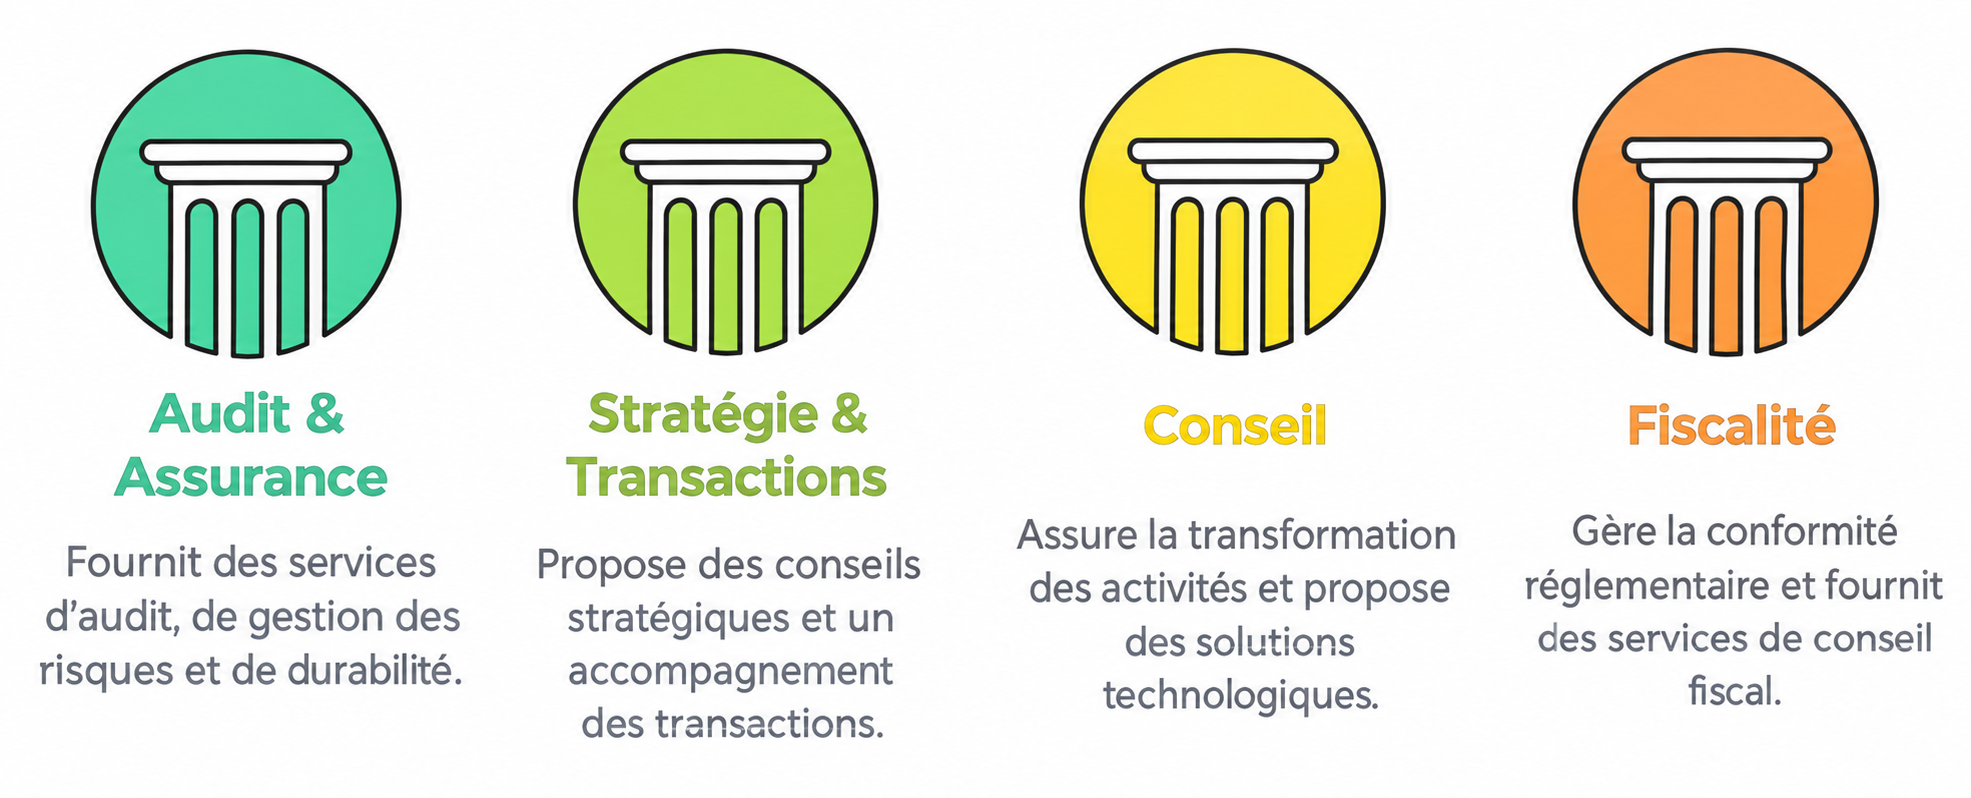
\includegraphics[width=0.25\textwidth]{figures/ey_logo.png}
    \caption{Logo du groupe EY \parencite{EYFY26}.}
    \label{fig:ey-logo}
\end{figure}

\subsection{Présentation d'EY Tunisie}

En Tunisie, EY est implanté depuis 1987 à travers son bureau de Tunis, sous la dénomination AMC Ernst \& Young. Le bureau compte plus de 900 professionnels, dont 23 associés, et couvre une dizaine de secteurs d'activité. Il y mène chaque année plus de 600 missions, couvrant une trentaine de pays. EY Tunisie y a notamment mis en place le premier laboratoire EY Cyber \& RPA en Tunisie, consacré à la cybersécurité et à l'automatisation robotisée des processus.

\subsection{Organisation et domaines d'activité}

L'activité d'EY Tunisie est organisée autour des quatre mêmes lignes de services qu'au niveau du groupe, présentées à la figure~\ref{fig:ey-lignes-service}. L'Assurance regroupe l'audit et les services associés, notamment en matière de risques financiers et de durabilité, au service de la fiabilité et de la transparence de l'information des clients. Le Consulting accompagne la transformation des organisations par la technologie, les données et l'intelligence artificielle, et couvre également des domaines tels que la cybersécurité et l'ingénierie digitale. La ligne Tax prend en charge la conformité fiscale des entreprises ainsi que le conseil en fiscalité internationale et en droit social. Strategy and Transactions, enfin, intervient dans les opérations de transaction, l'évaluation financière, les stratégies de croissance et les opérations de restructuration.

\begin{figure}[htbp]
    \centering
    
\includegraphics[width=0.85\textwidth]{figures/ey_quatre_lignes_service.png}
    \caption{Les quatre lignes de services d'EY Tunisie \parencite{EYFY26}.}
    \label{fig:ey-lignes-service}
\end{figure}

\subsection{Présentation de l'entité d'accueil}

Le stage à l'origine de ce rapport a été réalisé au sein de la ligne Consulting, et plus précisément de l'entité AI \& Data. C'est dans ce cadre qu'a été confiée la mission de gestion du risque de crédit bancaire présentée dans ce rapport.

\section{Contexte général du projet}

Le crédit constitue l'un des principaux leviers de financement de l'activité économique : il permet à des particuliers et à des entreprises de disposer de ressources qu'ils rembourseront progressivement, pour financer un investissement, une activité ou une consommation qu'ils ne pourraient pas couvrir avec leurs seules ressources immédiates. Pour la banque qui l'accorde, chaque crédit représente à la fois une source de revenus, à travers les intérêts perçus, et une exposition à un risque, celui de ne pas être intégralement remboursée. Développer les financements accordés tout en maîtrisant le risque associé constitue ainsi un équilibre que chaque banque doit rechercher en permanence, et qui conditionne directement sa solidité financière dans la durée.

Cet arbitrage repose sur quelques notions centrales. Le risque de crédit désigne la possibilité qu'un emprunteur ne respecte pas, en tout ou en partie, ses engagements de remboursement. Lorsque ce risque se matérialise, il se traduit par une perte, dont une partie est anticipée dès l'octroi du crédit : on parle alors de perte attendue, usuellement rapprochée de trois composantes : la probabilité de défaut de l'emprunteur (PD, \emph{Probability of Default}), la part de l'exposition qui ne serait pas recouvrée en cas de défaut (LGD, \emph{Loss Given Default}) et le montant de cette exposition au moment du défaut (EAD, \emph{Exposure at Default}), soit, sous une forme simplifiée, la perte de crédit attendue (ECL, \emph{Expected Credit Loss}) peut être exprimée par la relation $ECL \approx PD \times LGD \times EAD$. Cette expression donne une intuition de la relation entre ces trois composantes ; elle ne représente pas l'ensemble des modalités de calcul prévues par la norme IFRS 9, présentée ci-après. Au-delà de cette perte attendue, la banque doit également se prémunir contre des pertes inattendues, plus rares mais potentiellement plus importantes : c'est notamment le rôle des fonds propres, qui permettent à la banque d'absorber ces pertes et de préserver sa solvabilité. La rentabilité d'un crédit dépend ainsi non seulement des revenus qu'il génère, mais aussi du coût du risque qu'il représente et du capital qu'il immobilise.

Cette gestion du risque de crédit ne relève pas uniquement de choix internes à la banque : elle s'inscrit dans un cadre réglementaire qui en encadre la mesure et le provisionnement. La norme comptable \textsc{IFRS 9}, publiée par l'\textit{International Accounting Standards Board} et entrée en vigueur le 1er janvier 2018, repose sur un modèle général de dépréciation qui distingue trois catégories d'expositions, appelées \emph{stages} \parencite{IASB2014IFRS9}. Les expositions dont la qualité de crédit ne s'est pas dégradée de façon significative depuis leur comptabilisation initiale (stage 1) donnent lieu à la comptabilisation des pertes de crédit attendues associées aux défauts susceptibles de survenir au cours des douze mois suivant la date de clôture. Dès qu'une augmentation significative du risque de crédit est constatée depuis la comptabilisation initiale (SICR, \emph{Significant Increase in Credit Risk}, stage 2), ou \emph{a fortiori} lorsque l'exposition est dépréciée pour risque de crédit (stage 3), la provision doit couvrir la perte attendue sur toute la durée de vie restante de l'exposition, ce qui peut en accroître le montant, puisque l'horizon de calcul couvre désormais toute la durée de vie restante de l'exposition. À ce cadre comptable s'ajoute un cadre prudentiel, issu des accords de Bâle et porté par le \textit{Basel Committee on Banking Supervision}, qui définit des exigences minimales de fonds propres, notamment calculées à partir des actifs pondérés par les risques, afin de renforcer la capacité des banques à absorber les pertes \parencite{BCBS2017Basel3}. Ce capital réglementaire, calculé selon des règles communes à l'ensemble des établissements soumis à ces accords, ne se confond pas avec le capital économique qu'une banque peut par ailleurs estimer en interne pour ses propres besoins de pilotage.

Le projet présenté dans ce rapport s'inscrit dans cet environnement bancaire, financier et réglementaire. Il couvre deux niveaux d'analyse complémentaires : l'évaluation d'une nouvelle demande de crédit, désignée dans la suite du rapport par le terme \emph{Origination}, et le suivi d'un portefeuille de crédits déjà accordés, désigné par \emph{Portfolio Analytics}.

\section{Problématique et objectifs}

\subsection{Constat et formulation de la problématique}

La gestion du risque de crédit implique plusieurs dimensions complémentaires : l'évaluation du risque associé à un financement, l'estimation des pertes potentielles qui peuvent en résulter, la prise en compte du capital nécessaire pour absorber les pertes inattendues et l'appréciation de la rentabilité qu'il procure à la banque. Ces dimensions interviennent à différentes étapes du cycle de vie d'un crédit, depuis l'étude d'une nouvelle demande jusqu'au suivi, dans la durée, des financements déjà accordés.

La problématique à laquelle répond ce projet peut ainsi être formulée de la façon suivante : comment mettre en relation l'évaluation du risque de crédit et l'analyse de la rentabilité, afin d'éclairer à la fois la décision d'octroi d'un nouveau crédit et le suivi d'un portefeuille de crédits déjà accordés ?

\subsection{Objectif général}

L'objectif général de ce projet est de concevoir une plateforme d'aide à la décision permettant d'intégrer les dimensions du risque et de la rentabilité dans deux contextes complémentaires : l'évaluation des nouvelles demandes de crédit et le suivi des portefeuilles de crédits existants.

\subsection{Objectifs spécifiques}

Cet objectif général se décline en plusieurs objectifs spécifiques :

\begin{itemize}
    \item évaluer le risque associé à une nouvelle demande de crédit ;
    \item estimer les pertes attendues et prendre en compte le capital nécessaire à l'analyse de la rentabilité du dossier ;
    \item produire des éléments d'aide à la décision pour l'octroi des financements ;
    \item suivre et analyser, pour un portefeuille de crédits déjà accordés, le risque, les pertes attendues, le capital mobilisé et la rentabilité dans la durée ;
    \item présenter ces résultats sous forme d'indicateurs et d'analyses directement exploitables par les utilisateurs métier.
\end{itemize}

\section{Étude et critique de l'existant}

Pour situer le projet par rapport à l'existant, cette section compare trois solutions commerciales reconnues sur le marché de la gestion du risque de crédit : SAS, Moody's Analytics et FICO. Plutôt que de dresser un inventaire exhaustif de leurs fonctionnalités, l'analyse qui suit dégage, pour chacune, son positionnement, ses apports documentés et ses limites telles qu'elles ressortent de leur documentation officielle (tableau~\ref{tab:etude-existant}). Cette analyse comporte une limite méthodologique qu'il convient d'assumer explicitement : une fonctionnalité non mentionnée dans la documentation publique consultée ne peut être considérée comme inexistante dans l'offre réelle de l'éditeur.

\begin{table}[htbp]
    \centering
    \footnotesize
    \caption{Étude critique de trois solutions commerciales de gestion du risque de crédit.}
    \label{tab:etude-existant}
    \begin{tabular}{p{1.8cm}p{2.7cm}p{3cm}p{3.5cm}p{3.3cm}}
        \toprule
        \textbf{Solution} & \textbf{Positionnement} & \textbf{Points forts documentés} & \textbf{Limites et points de vigilance} & \textbf{Enseignements pour le projet} \\
        \midrule
        SAS \parencite{SASIFRS9} &
        Provisionnement et conformité IFRS 9 (ECL, classification par \emph{stage}). &
        Modèles PD/LGD préconstruits ; automatisation du calcul des ECL par scénario. &
        Documentation centrée sur le provisionnement comptable, sans détail sur le capital réglementaire ou la rentabilité par dossier. &
        Confirme la maturité attendue sur l'IFRS 9, à relier explicitement à la rentabilité du dossier. \\
        \addlinespace
        Moody's Analytics \parencite{MoodysIFRS9} &
        Souscription, surveillance de portefeuille et modélisation IFRS 9, via plusieurs produits dédiés. &
        Scénarios macroéconomiques sur plus de 70 pays ; \emph{staging} IFRS 9 documenté ; usage cité pour le capital interne au risque. &
        Les produits sont présentés séparément dans la documentation consultée, qui ne met pas explicitement en évidence un flux unique reliant octroi et suivi de portefeuille. &
        Couverture fonctionnelle large, que le projet cherche à relier dans un même processus. \\
        \addlinespace
        FICO \parencite{FICOOriginations} &
        Décisionnel d'octroi : stratégies combinant risque de crédit et détection de fraude. &
        Configuration des stratégies en \emph{low-code} ; risque et fraude dans une même couche décisionnelle. &
        Documentation centrée sur l'octroi, sans détail sur le suivi du portefeuille dans la durée. &
        Confirme l'intérêt d'un décisionnel d'octroi structuré, complété par un suivi de portefeuille. \\
        \bottomrule
    \end{tabular}
\end{table}

Cette comparaison met en évidence des positionnements complémentaires : SAS met l'accent sur le provisionnement IFRS 9, Moody's Analytics propose plusieurs solutions couvrant différentes dimensions de la gestion du risque, tandis que FICO se concentre notamment sur le décisionnel d'octroi. Les documentations étudiées ne mettent toutefois pas explicitement en évidence une démarche réunissant l'évaluation du risque, l'analyse de la rentabilité, la décision d'octroi et le suivi du portefeuille dans un même processus. Ce constat, limité aux informations publiquement documentées, permet de situer le positionnement du projet présenté dans ce rapport.

\section{Solution proposée}

La solution proposée dans ce rapport est une plateforme d'aide à la décision qui met en regard, pour un crédit comme pour un portefeuille déjà constitué, le risque qu'il représente et la rentabilité qu'il procure à la banque, occupant ainsi l'espace mis en évidence à l'issue de l'étude de l'existant. Elle se décline en deux volets complémentaires : \emph{Origination}, qui couvre l'évaluation d'une nouvelle demande de crédit jusqu'à la décision d'octroi, et \emph{Portfolio Analytics}, qui couvre le suivi d'un portefeuille de crédits déjà accordés. Les deux volets s'appuient sur un socle commun d'évaluation du risque, sans que leurs calculs soient nécessairement identiques : le capital mobilisé, par exemple, ne se détermine pas selon le même mécanisme pour un dossier individuel et pour un portefeuille.

Dans les deux cas, la plateforme suit le même enchaînement fonctionnel : évaluation du risque, estimation des pertes attendues, puis prise en compte du capital nécessaire pour absorber d'éventuelles pertes inattendues et de la rentabilité du financement, pour aboutir à un résultat exploitable. Ce résultat prend la forme d'une décision d'octroi assortie de ses justifications pour \emph{Origination}, et d'un ensemble d'indicateurs portant sur le risque, les pertes attendues, le capital mobilisé et la rentabilité du portefeuille, calculés à intervalles réguliers pour \emph{Portfolio Analytics}, indépendamment des décisions d'octroi : ce suivi ne découle pas automatiquement de chaque décision. Les besoins qui en découlent sont précisés au chapitre~2, les traitements métier et techniques aux chapitres~3 à 6, et l'architecture de la plateforme au chapitre~5.

\section{Méthodologie utilisée}

\subsection{Principes d'une démarche itérative et incrémentale}

Une démarche itérative et incrémentale repose sur deux principes distincts, souvent évoqués ensemble mais qui ne se confondent pas \parencite{LarmanBasili2003}. Le principe itératif consiste à revenir, au fil de cycles de travail successifs, sur des éléments déjà réalisés, afin de les affiner ou de les corriger à la lumière de nouveaux résultats. Le principe incrémental consiste, de son côté, à construire la solution par ajouts progressifs : chaque étape complète ce qui a déjà été réalisé, sans nécessairement tout reprendre depuis le début. Associés, ces deux principes permettent de faire évoluer une solution progressivement, tout en conservant la possibilité de revenir sur des choix antérieurs lorsque leur vérification le justifie, comme l'illustre la figure~\ref{fig:cycle-iteratif}. C'est selon ces deux principes que ce projet a été conduit.

\begin{figure}[htbp]
    \centering
    \begin{tikzpicture}[
        box/.style={draw, rounded corners, align=center, minimum width=3.4cm, minimum height=1.2cm, font=\footnotesize, fill=gray!10},
        arrow/.style={-{Latex[length=2.5mm]}, thick}
    ]
        \node[box] (top) at (0,3) {Réalisation incrémentale\\(ajout d'un élément)};
        \node[box] (right) at (4,0) {Vérification};
        \node[box] (bottom) at (0,-3) {Ajustement itératif\\(reprise si nécessaire)};
        \node[box] (left) at (-4,0) {Consolidation};
        \node[align=center, font=\footnotesize\itshape] at (0,0) {Évolution progressive\\de la solution};
        \draw[arrow] (top.east) to[bend left=25] (right.north);
        \draw[arrow] (right.south) to[bend left=25] (bottom.east);
        \draw[arrow] (bottom.west) to[bend left=25] (left.south);
        \draw[arrow] (left.north) to[bend left=25] (top.west);
    \end{tikzpicture}
    \caption{Schéma illustrant le principe itératif et incrémental retenu pour ce projet (illustration personnelle).}
    \label{fig:cycle-iteratif}
\end{figure}

\subsection{Phases de la démarche suivie}

Le travail s'est organisé autour de quatre grandes phases, résumées dans le tableau~\ref{tab:phases-demarche}. Ces phases ne se sont pas succédé de façon strictement linéaire : une vérification menée dans l'une d'elles pouvait remettre en cause une décision prise lors d'une phase antérieure, qu'il fallait alors reprendre avant de poursuivre.

\begin{table}[htbp]
    \centering
    \footnotesize
    \caption{Phases de la démarche suivie.}
    \label{tab:phases-demarche}
    \begin{tabular}{p{3.2cm}p{5cm}p{6cm}}
        \toprule
        \textbf{Phase} & \textbf{Objectif} & \textbf{Travaux réalisés} \\
        \midrule
        Compréhension du besoin et cadrage &
        Analyser le contexte métier du risque de crédit et délimiter le périmètre du projet. &
        Étude du cadre réglementaire et financier, identification des besoins, définition des deux volets du projet. \\
        \addlinespace
        Préparation et constitution des données &
        Réunir et préparer les données nécessaires à l'évaluation du risque. &
        Nettoyage des données réelles disponibles, génération de données synthétiques de comportement de défaut, calibration et vérification de ces données. \\
        \addlinespace
        Conception et développement des traitements &
        Concevoir et développer les traitements d'évaluation du risque, de quantification financière et d'aide à la décision. &
        Construction des modèles de score de crédit, calculs de pertes attendues, de capital et de rentabilité, mécanismes de décision et de pilotage. \\
        \addlinespace
        Vérification et amélioration &
        Évaluer la cohérence et la fiabilité des traitements développés. &
        Audits de cohérence, tests sur les traitements métier et sur leur intégration. \\
        \bottomrule
    \end{tabular}
\end{table}

Deux vérifications menées au cours de ces phases illustrent concrètement cette démarche. Lors de la préparation des données, un audit du processus de génération des données synthétiques du segment Entreprises a mis en évidence un taux cible de défaut trop élevé au regard du comportement attendu du segment ; ce taux a été revu à la baisse et la génération des données reprise en conséquence. Lors de la conception des traitements, l'évaluation d'un des algorithmes candidats au score de crédit du segment Particuliers, sur un jeu de test organisé selon un découpage temporel, a révélé une forte dégradation de ses performances, mettant en évidence une capacité de généralisation insuffisante sur des données temporellement plus récentes ; cet algorithme a été écarté du choix final au profit des deux autres candidats retenus. Une correction motivée par l'une des vérifications de la dernière phase a par ailleurs pu être répercutée sur des livrables antérieurs déjà considérés comme aboutis, lorsqu'elle concernait un élément qu'ils réutilisaient.

\subsection{Bénéfices de la démarche suivie}

Une démarche itérative et incrémentale est généralement présentée, dans les principes qui la définissent, comme permettant de détecter plus tôt les incohérences et les erreurs, de valider progressivement les choix retenus plutôt que de les découvrir en bloc en fin de projet, et de s'adapter à des exigences qui ne sont pas toutes connues ni figées dès le départ. Dans le cadre de ce projet, cette démarche a permis de confronter progressivement les choix effectués aux résultats obtenus et de les ajuster lorsque les vérifications le nécessitaient. Les reprises réalisées ont ainsi contribué à corriger les incohérences détectées et à renforcer la cohérence entre les différentes composantes de la plateforme. Elles ont également permis de fonder les décisions de développement sur des résultats contrôlés plutôt que sur des hypothèses non vérifiées.

\section*{Conclusion du chapitre}

Ce chapitre a situé le projet présenté dans ce rapport : réalisé au sein de l'entité AI \& Data d'EY Tunisie, il répond à un besoin de rapprocher l'évaluation du risque de crédit et l'analyse de la rentabilité, dans un environnement bancaire structuré par les normes IFRS 9 et Bâle. L'étude de trois solutions commerciales existantes a montré que les documentations consultées ne mettent pas explicitement en évidence une approche réunissant ces deux dimensions, aussi bien pour l'octroi d'un nouveau crédit que pour le suivi d'un portefeuille existant. C'est cet espace que la plateforme proposée, déclinée en deux volets complémentaires, \emph{Origination} et \emph{Portfolio Analytics}, cherche à occuper. Sa réalisation a suivi une démarche itérative et incrémentale, dont les phases et les ajustements ont été détaillés dans ce chapitre. Le chapitre suivant précise les besoins fonctionnels et non fonctionnels qui découlent de ce cadrage, ainsi que les utilisateurs auxquels la plateforme s'adresse.

\chapter{Analyse et spécification des besoins}

Après avoir posé le contexte et la problématique au chapitre précédent, ce chapitre fait le lien entre ce cadre général et la construction de la plateforme elle-même. Il identifie les acteurs auxquels celle-ci s'adresse et les responsabilités métier qui leur sont associées, avant de spécifier les besoins fonctionnels et non fonctionnels qui en découlent. Une modélisation des cas d'utilisation referme ce chapitre, en formalisant les interactions entre ces acteurs et les principales fonctionnalités de la plateforme, que les chapitres suivants détaillent progressivement.

\section{Analyse des besoins, acteurs et rôles}

Le chapitre précédent a présenté la problématique et les objectifs de ce projet : rapprocher l'évaluation du risque et l'analyse de la rentabilité, au service de la décision d'octroi et du pilotage du portefeuille. Cette section identifie les acteurs auxquels la plateforme s'adresse et les responsabilités métier qui leur sont associées, telles qu'elles sont effectivement prises en charge par la plateforme.

Le \emph{Chargé de clientèle}, responsable de la relation avec les clients qui lui sont affectés, initie les demandes de crédit et en suit le traitement. Il dispose d'un accès aux informations générales, aux décisions et aux revues de risque, mais pas aux données quantitatives du risque, telles que la probabilité de défaut ou les facteurs explicatifs d'une décision, qui relèvent d'une analyse plus spécialisée. L'\emph{Analyste crédit} instruit également les demandes de crédit, mais sur le plan de l'analyse du risque : il dispose, à ce titre, d'un accès aux indicateurs quantitatifs du risque, notamment la probabilité de défaut, la perte en cas de défaut, les pertes attendues et les facteurs explicatifs d'une décision, en plus des éléments déjà accessibles au Chargé de clientèle.

Le \emph{Risk Manager} occupe une position centrale dans le dispositif : il valide les décisions de crédit qui dépassent le seuil délégué aux deux acteurs précédents, intervient dans les décisions prises en comité de crédit, et pilote l'analyse du portefeuille (risque, pertes, capital, rentabilité) dans la durée. Son accès aux données de la plateforme est, en conséquence, le plus complet.

La \emph{Direction} dispose d'un accès en lecture à des synthèses agrégées de portefeuille et à des indicateurs stratégiques, sans intervenir dans le traitement d'un dossier individuel ni dans les décisions d'octroi. La \emph{Conformité et l'Audit} consultent a posteriori les décisions prises et leur traçabilité, afin d'en contrôler la cohérence, sans participer eux-mêmes à ces décisions. L'\emph{Administrateur}, enfin, gère les aspects techniques de la plateforme (utilisateurs, rôles et configuration). Ses responsabilités relèvent de l'administration du système. Il ne dispose pas du pouvoir de validation individuelle des crédits, mais peut intervenir dans le processus collégial de décision en comité, conformément aux autorisations prévues dans la plateforme.

Le tableau~\ref{tab:acteurs-roles} résume ces responsabilités et leur correspondance avec les rôles effectivement définis dans la plateforme.

\begin{table}[htbp]
    \centering
    \footnotesize
    \caption{Acteurs de la plateforme et responsabilités principales.}
    \label{tab:acteurs-roles}
    \begin{tabular}{p{3.2cm}p{7cm}p{3.5cm}}
        \toprule
        \textbf{Acteur} & \textbf{Responsabilités principales} & \textbf{Rôle correspondant} \\
        \midrule
        Chargé de clientèle & Initie et suit les demandes de crédit de ses clients. & \texttt{RELATIONSHIP\_MGR} \\
        \addlinespace
        Analyste crédit & Instruit les demandes de crédit et en analyse le risque. & \texttt{CREDIT\_ANALYST} \\
        \addlinespace
        Risk Manager & Valide les décisions, décide en comité de crédit, pilote le portefeuille. & \texttt{RISK\_MANAGER} \\
        \addlinespace
        Direction & Consulte des synthèses stratégiques agrégées du portefeuille. & \texttt{EXECUTIVE} \\
        \addlinespace
        Conformité / Audit & Contrôle a posteriori la traçabilité des décisions. & \texttt{COMPLIANCE\_AUDIT} \\
        \addlinespace
        Administrateur & Gère les aspects techniques de la plateforme. & \texttt{ADMIN} \\
        \bottomrule
    \end{tabular}
\end{table}

\section{Spécification des besoins fonctionnels}

\subsection{Gestion des demandes de crédit (Origination)}

Les acteurs intervenant dans le processus d'octroi, le Chargé de clientèle et l'Analyste crédit, doivent pouvoir saisir une nouvelle demande de crédit, l'instruire avec les informations nécessaires à son évaluation, puis accéder à une décision d'octroi justifiée, assortie des éléments de risque et de rentabilité qui la motivent.

\subsection{Évaluation du risque et des pertes}

La plateforme doit produire les indicateurs quantitatifs nécessaires à l'analyse du risque, à la fois pour un dossier individuel lors de son instruction, et pour un portefeuille de crédits déjà accordés lors de son suivi, sans que ces deux évaluations reposent nécessairement sur les mêmes mécanismes de calcul. Pour un dossier individuel, ce besoin consiste à évaluer le risque de l'emprunteur et à estimer les pertes attendues et le capital pris en compte dans l'analyse, selon les mécanismes retenus pour l'Origination. Pour un portefeuille, il consiste à analyser les pertes attendues et le capital mobilisé à l'échelle du portefeuille, en tenant compte de son exposition globale.

\subsection{Analyse et pilotage du portefeuille (Portfolio Analytics)}

Le Risk Manager doit pouvoir suivre l'évolution du portefeuille dans le temps et en analyser les principales caractéristiques, à partir des indicateurs produits par l'évaluation du risque. La Direction doit, quant à elle, disposer d'une vision synthétique et agrégée de cette évolution.

\subsection{Analyse du capital, de la rentabilité et aide à la décision}

La plateforme doit mettre en relation le risque, les pertes attendues, le capital et la rentabilité, afin d'éclairer, d'une part, la décision d'octroi d'un dossier individuel, notamment lors des validations et des interventions en comité de crédit prévues par les seuils de délégation présentés en section~2.1, et, d'autre part, le pilotage du portefeuille dans son ensemble.

\subsection{Assistant intelligent}

La plateforme doit permettre aux utilisateurs d'interroger, en langage naturel, les informations et résultats qu'elle produit, dans les limites des données et des fonctionnalités auxquelles leur rôle leur donne accès. Cet assistant reste une fonctionnalité consultative : il n'intervient dans aucune décision et ne garantit pas de répondre à toute question qui lui est posée.

\section{Spécification des besoins non fonctionnels}

\subsection{Sécurité et contrôle d'accès}

Chaque utilisateur ne doit accéder qu'aux fonctionnalités correspondant à son rôle, et qu'aux données couvertes par les autorisations associées à ce rôle, selon la répartition des responsabilités présentée en section~2.1.

\subsection{Traçabilité et auditabilité}

La plateforme doit assurer la traçabilité des traitements et des décisions significatifs, notamment les opérations d'ingestion, de transformation, d'entraînement et de décision de crédit. Les événements enregistrés doivent pouvoir être vérifiés a posteriori, et leur intégrité doit être protégée contre toute modification silencieuse.

\subsection{Fiabilité et cohérence des calculs}

Les résultats produits doivent respecter la cohérence des relations entre les indicateurs de risque, les pertes attendues, le capital et la rentabilité. Les calculs doivent également être reproductibles à partir des mêmes données et des mêmes paramètres.

\subsection{Gestion des volumes de données}

La plateforme doit pouvoir traiter les données des segments Particuliers et Entreprises dans des délais compatibles avec les traitements périodiques prévus pour l'évaluation du risque et le suivi du portefeuille.

\subsection{Modularité et maintenabilité}

Les composants d'évaluation du risque, de quantification financière et d'aide à la décision doivent pouvoir évoluer indépendamment les uns des autres.

\section{Modélisation des cas d'utilisation}

La figure~\ref{fig:cas-utilisation} présente les interactions entre les six acteurs identifiés en section~2.1 et les principales fonctionnalités de la plateforme, regroupées en cinq ensembles fonctionnels correspondant aux principaux parcours de la plateforme : l'évaluation d'une demande de crédit (Origination), l'arbitrage et le comité de crédit, l'analyse du portefeuille (Portfolio Analytics), la gouvernance et l'audit, et l'assistant conversationnel, transversal aux six acteurs. Les associations entre acteurs et cas d'utilisation reflètent directement les autorisations réellement définies dans la plateforme.

\begin{figure}[htbp]
    \centering
    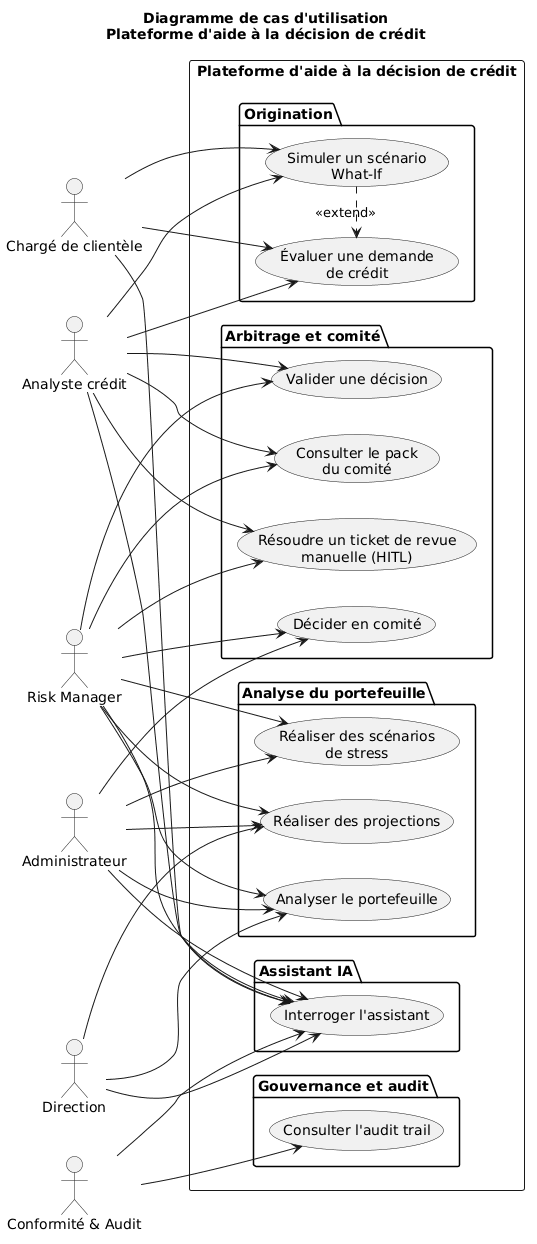
\includegraphics[width=\textwidth,height=0.85\textheight,keepaspectratio]{figures/diagramme_cas_utilisation_v2.png}
    \caption{Diagramme de cas d'utilisation de la plateforme (élaboration personnelle, à partir des rôles et autorisations réellement implémentés).}
    \label{fig:cas-utilisation}
\end{figure}

Parmi ces cas d'utilisation, quatre concentrent l'essentiel de la valeur métier de la plateforme et sont décrits plus en détail dans le tableau~\ref{tab:cas-utilisation-prioritaires}.

\begin{table}[htbp]
    \centering
    \footnotesize
    \caption{Description des cas d'utilisation prioritaires.}
    \label{tab:cas-utilisation-prioritaires}
    \begin{tabular}{p{3cm}p{3cm}p{8cm}}
        \toprule
        \textbf{Cas d'utilisation} & \textbf{Acteur(s)} & \textbf{Description} \\
        \midrule
        Évaluer une demande de crédit &
        Chargé de clientèle, Analyste crédit &
        Saisir une nouvelle demande de crédit et en obtenir l'évaluation du risque, jusqu'à une décision d'octroi justifiée. Ce cas d'utilisation peut être étendu par la simulation d'un scénario \emph{What-If}, qui permet de recalculer cette évaluation pour des paramètres de la demande modifiés par l'utilisateur, sans enregistrer le résultat dans le système. \\
        \addlinespace
        Valider une décision / Décider en comité &
        Risk Manager (validation seule) ; Risk Manager et Administrateur (décision en comité) &
Statuer sur les demandes dont la décision dépasse le niveau de délégation accordé au Chargé de clientèle et à l'Analyste crédit. Une décision individuelle est validée par le Risk Manager seul ; une décision collégiale, prise en comité de crédit, peut associer l'Administrateur à la décision du Risk Manager. \\
        \addlinespace
        Résoudre un ticket de revue manuelle &
        Analyste crédit, Risk Manager &
        Traiter un dossier signalé pour un examen humain (par exemple une incohérence ou une limite atteinte par l'évaluation automatisée), jusqu'à sa résolution. \\
        \addlinespace
        Analyser le portefeuille &
        Risk Manager, Direction &
        Consulter l'évolution du risque, des pertes attendues, du capital mobilisé et de la rentabilité d'un portefeuille de crédits déjà accordés, notamment à travers des projections et des scénarios de stress. \\
        \bottomrule
    \end{tabular}
\end{table}

\section*{Conclusion du chapitre}

Ce chapitre a traduit le cadrage posé au chapitre précédent en besoins concrets. Six acteurs ont été identifiés, chacun avec des responsabilités et des droits d'accès qui lui sont propres, de l'instruction d'une demande de crédit au contrôle a posteriori des décisions prises. Les besoins fonctionnels couvrent les deux volets de la plateforme, Origination et Portfolio Analytics, ainsi que l'assistant intelligent qui les accompagne ; les besoins non fonctionnels portent sur la sécurité, la traçabilité, la fiabilité des calculs, les volumes de données et la maintenabilité des composants. La modélisation des cas d'utilisation a permis de représenter ces besoins sous la forme des interactions réellement autorisées entre les acteurs et la plateforme. Le chapitre suivant aborde la préparation des données et la construction des modèles prédictifs qui contribuent à l'évaluation du risque.

\chapter{Préparation des données et modélisation du risque de crédit}

Ce chapitre présente les données mobilisées pour ce projet et leur transformation progressive en modèles de risque exploitables. Il part de la source unique dont dispose le projet, en expose la compréhension, le nettoyage et la construction de la variable cible, avant de détailler le développement des modèles de probabilité de défaut puis de perte en cas de défaut. Il se referme sur l'évaluation, la sélection et l'interprétabilité de ces modèles, dont les artefacts entraînés sont ensuite exploités pour la quantification du risque présentée au chapitre suivant.

\section{Compréhension et exploration des données}

\subsection{Présentation de la source des données}

Les données utilisées dans ce projet proviennent d'un unique fichier source réel, \texttt{Base\_depot.xlsx}, extrait du système d'information bancaire. Ce fichier contient des comptes de dépôt, et non des données de crédit : il sert de point d'ancrage, en fournissant une structure de clientèle réelle, clients, comptes, agences et encours, à partir de laquelle les données nécessaires à l'étude du risque de crédit ont ensuite été construites.

\subsection{Description du jeu de données}

Le tableau~\ref{tab:donnees-source} résume les principales caractéristiques de ce jeu de données, avant et après nettoyage.

\begin{table}[htbp]
    \centering
    \footnotesize
    \caption{Chiffres de référence du jeu de données source.}
    \label{tab:donnees-source}
    \begin{tabular}{p{7cm}p{4cm}}
        \toprule
        \textbf{Indicateur} & \textbf{Valeur} \\
        \midrule
        Lignes brutes & 211 825 \\
        Lignes après nettoyage & 211 824 \\
        Clients uniques & 154 619 \\
        Comptes uniques & 211 824 \\
        Agences uniques & 50 \\
        Catégorie à encours élevé (assimilée au segment Entreprises dans la simulation) & 556 clients (0,36\,\%), représentant 40,1\,\% de l'encours total \\
        Catégorie à encours standard (assimilée au segment Particuliers dans la simulation) & 154 063 clients (99,64\,\%), représentant 59,9\,\% de l'encours total \\
        \bottomrule
    \end{tabular}
\end{table}

Cette répartition ne correspond pas à une classification juridique des clients présente dans la source : elle a été construite à partir de leur niveau d'encours afin de définir deux catégories utilisées dans la simulation.

\subsection{Limites de la source et recours aux données synthétiques}

Cette source présente une limite déterminante pour la suite du projet : elle ne contient ni historique de crédit, ni défaut observé, seulement des comptes de dépôt. Les informations relatives aux crédits eux-mêmes, octroi, remboursement, défaut, n'existent donc pas dans les données réelles : elles ont été générées synthétiquement, à partir de la structure réelle de la clientèle et des comptes présentée ci-dessus. Les modèles prédictifs présentés dans la suite de ce chapitre n'ont ainsi pas été entraînés sur des défauts bancaires historiquement observés, mais sur des historiques de défaut générés et calibrés dans ce cadre, dont la construction est détaillée en section~3.3.

\subsection{Traitement des encours négatifs}

Parmi les comptes de la source réelle, 850 présentent un solde d'encours négatif. Ces comptes ont été conservés, plutôt qu'exclus ou corrigés, et signalés par un indicateur dédié : un encours négatif peut constituer une information comportementale potentiellement utile, qu'il aurait été dommageable de supprimer. Cette conservation ne préjuge toutefois pas de la nature de ces encours négatifs, qui ne correspondent pas nécessairement à un incident de paiement.

\section{Nettoyage, qualité et préparation des données}

\subsection{Nettoyage du fichier source}

Le fichier source présente plusieurs anomalies traitées lors de sa préparation. Neuf colonnes présentent un taux de remplissage réel de 0~\% et sont supprimées : le choix a été de ne pas les imputer, aucun contenu réel ne permettant de justifier une valeur imputée. Une ligne contient par ailleurs un en-tête de colonne inséré accidentellement lors d'une exportation ; elle est supprimée par un filtre sur la devise. C'est cette même ligne qui présente l'unique valeur d'encours manquante du fichier, également supprimée par ce filtre. Les encours négatifs, traités séparément, ont été présentés en section~3.1.

\subsection{Construction de la variable de segmentation}

Pour distinguer les clients des segments Particuliers et Entreprises, introduits en section~3.1, une variable d'encours agrégé par client est d'abord calculée, en sommant l'encours de l'ensemble des comptes qu'il détient, y compris ses éventuels encours négatifs. Un client est affecté au segment Entreprises (simulé) si cet encours agrégé atteint ou dépasse 50 millions de XOF, et au segment Particuliers (simulé) en deçà de ce seuil.

Ce seuil a été retenu après une analyse de sensibilité portant sur huit valeurs candidates, dont les résultats sont résumés dans le tableau~\ref{tab:seuil-segmentation}. Pour chacune, l'écart entre l'encours minimum du segment Entreprises et l'encours maximum du segment Particuliers a été mesuré.

\begin{table}[htbp]
    \centering
    \footnotesize
    \caption{Analyse de sensibilité du seuil de segmentation.}
    \label{tab:seuil-segmentation}
    \begin{tabular}{p{2.2cm}p{2.8cm}p{1.8cm}p{1.8cm}p{2.8cm}}
        \toprule
        \textbf{Seuil} & \textbf{Clients segment élevé} & \textbf{\% clients} & \textbf{\% encours} & \textbf{Écart de séparation} \\
        \midrule
        10 M XOF & 4 789 & 3,10\,\% & 68,4\,\% & 100 XOF \\
        20 M XOF & 1 993 & 1,29\,\% & 55,1\,\% & 2 063 XOF \\
        30 M XOF & 1 149 & 0,74\,\% & 48,0\,\% & 24 013 XOF \\
        40 M XOF & 764 & 0,49\,\% & 43,3\,\% & 41 276 XOF \\
        \textbf{50 M XOF} & \textbf{556} & \textbf{0,36\,\%} & \textbf{40,1\,\%} & \textbf{87 369 XOF} \\
        60 M XOF & 420 & 0,27\,\% & 37,5\,\% & 268 992 XOF \\
        75 M XOF & 304 & 0,20\,\% & 34,8\,\% & 493 012 XOF \\
        100 M XOF & 201 & 0,13\,\% & 31,7\,\% & 132 188 XOF \\
        \bottomrule
    \end{tabular}
\end{table}

À tous les seuils testés sur ces données, cet écart est positif, ce qui indique, sur les données étudiées, une séparation nette entre les deux populations plutôt qu'un chevauchement continu. Le seuil de 50 millions de XOF a été retenu comme compromis entre l'écart de séparation obtenu, la part d'encours qu'il permet d'isoler (40,1~\%) et le nombre de clients regroupés dans chaque segment.

Cette segmentation reste une règle de simulation, configurable, et non une classification juridique des clients : le fichier source ne contient aucune variable permettant d'identifier le statut juridique d'un client, et ce seuil sert de proxy opérationnel.

\subsection{Construction des variables explicatives et prévention des fuites de données}

Les variables explicatives sont construites séparément pour chaque segment (respectivement dans \texttt{retail\_features.py} et \texttt{corporate\_features.py}), selon trois catégories communes : des variables statiques, connues au moment de l'octroi ; des variables comportementales pour le segment Particuliers, ou de migration de rating pour le segment Entreprises, qui retracent l'historique du client jusqu'à la date d'observation ; et des variables macroéconomiques, propres à cette même date.

La construction de ces variables applique trois règles destinées à éviter toute fuite d'information entre les données disponibles au moment de la prédiction et celles utilisées pour l'évaluer. La variable de probabilité de défaut initiale est systématiquement exclue des variables explicatives. Le défaut à prédire, détaillé en section~3.3, est calculé sur une fenêtre strictement postérieure à la date d'observation : douze mois pour le segment Particuliers, quatre trimestres pour le segment Entreprises. Enfin, les comptes déjà en défaut à la date d'observation sont exclus, leur label n'étant pas défini.

\subsection{Organisation du Feature Store pour la modélisation}

Les variables ainsi construites sont organisées en deux pipelines distincts, l'un pour le segment Particuliers, l'autre pour le segment Entreprises. Cette séparation tient à la nature même des deux segments : leurs temporalités d'observation, mensuelle pour l'un, trimestrielle pour l'autre, ainsi que leurs variables explicatives, ne sont pas les mêmes, ce qui rend un traitement commun inapproprié.

Le choix de ces deux fréquences répond également à la nature des informations suivies. Pour les Particuliers, l'observation mensuelle permet de suivre les retards de paiement au rythme des échéances des crédits amortissables. Pour les Entreprises, le suivi repose davantage sur des ratios financiers et sur l'évolution de la notation, construits à partir d'informations comptables et financières dont l'actualisation n'est pas nécessairement mensuelle. Une granularité trimestrielle a donc été retenue dans le générateur afin de représenter cette évolution à un rythme adapté aux variables mobilisées. Ces fréquences constituent ainsi des choix de modélisation propres aux deux segments, et non des paramètres issus d'une comparaison expérimentale entre plusieurs cadences.

Les modèles construits à partir de ces deux pipelines sont présentés en section~3.4.

\section{Construction de la variable cible}

\subsection{Définition de l'événement de défaut}

Le défaut d'un client est défini différemment selon le segment, tout en reposant sur une logique commune : la confirmation de la dégradation sur plusieurs périodes consécutives, plutôt que sur un seul constat ponctuel. Pour le segment Particuliers, un client est considéré en défaut après trois mois consécutifs de retard de paiement sévère, de 90 jours ou plus. Pour le segment Entreprises, dont le suivi est trimestriel, un client est considéré en défaut après deux trimestres consécutifs dans la catégorie de notation CCC\_D, qui représente le niveau le plus dégradé de l'échelle retenue.

\subsection{Génération des historiques synthétiques}

En l'absence d'historique de crédit réel, rappelée en section~3.1, les trajectoires de remboursement et de défaut des clients ont été générées par simulation, à l'aide de chaînes de Markov : chaque client évolue, période après période, entre plusieurs états représentant son niveau de retard de paiement pour les Particuliers, ou sa notation pour les Entreprises, selon des probabilités de transition calibrées pour chaque segment. Ces transitions sont rendues sensibles à des variables macroéconomiques, le chômage et la croissance pour le segment Particuliers, la croissance et des taux propres à chaque secteur d'activité pour le segment Entreprises, de sorte que la probabilité de dégradation d'un client varie avec le contexte économique simulé plutôt que de rester constante dans le temps. Le détail des états et des matrices de transition retenues est présenté en annexe~C.

Les probabilités de transition sont calibrées autour de taux de défaut cibles de 7~\% pour le segment Particuliers et de 9~\% pour le segment Entreprises, à l'échelle des populations simulées. Ces taux cibles de calibration ne doivent pas être confondus avec le taux de défaut mesuré dans les échantillons d'évaluation des modèles, présenté en section~3.6, qui constitue une grandeur différente. Le taux cible du segment Entreprises a par ailleurs été révisé de 14~\% à 9~\%, après qu'une vérification du générateur a révélé une anomalie dans le mécanisme de simulation des notations. Après correction, le taux de 9~\% a été retenu comme valeur de calibration cohérente avec le comportement du générateur corrigé, et non comme un ajustement destiné à obtenir un résultat prédéfini.

\subsection{Construction des observations et horizons prédictifs}

Les trajectoires ainsi simulées sont ensuite observées à intervalles réguliers, un snapshot mensuel pour le segment Particuliers, trimestriel pour le segment Entreprises, afin de constituer les observations utilisées pour la modélisation. Chaque snapshot associe, à un client et à une date donnée, les variables explicatives construites en section~3.2 et l'indication de survenue ou non d'un défaut au cours de l'horizon prédictif suivant cette date : douze mois pour les Particuliers, quatre trimestres pour les Entreprises.

\section{Développement des modèles de PD}

\subsection{Démarche de modélisation}

Pour chaque segment, Particuliers et Entreprises, plusieurs algorithmes candidats sont entraînés et évalués selon un protocole commun, afin de retenir un modèle champion ; les autres algorithmes évalués sont conservés à titre de challengers. Cette architecture champion/challenger permet de documenter la comparaison entre plusieurs approches plutôt que de présenter un algorithme unique sans alternative examinée.

Le protocole appliqué à chaque algorithme candidat d'un même segment est identique : mêmes variables explicatives, mêmes jeux d'entraînement, de calibration et de test, et mêmes métriques d'évaluation, détaillées en section~3.6. Pour les modèles présentés dans cette section, qui répondent au besoin du suivi de portefeuille, le champion est désigné automatiquement parmi les candidats évalués, en retenant celui dont l'aire sous la courbe ROC (AUC), calculée sur le jeu de test, est la plus élevée. Le pipeline distinct propre à l'Origination, présenté en section~3.7, retient une démarche de sélection différente.

Cette méthode appelle une réserve méthodologique qu'il convient d'exposer clairement plutôt que de l'omettre. Le jeu de test sert à la fois à sélectionner le champion et à rapporter les performances finales de ce même champion, présentées en section~3.6. Cette double utilisation introduit un risque d'optimisme dans l'estimation de ces performances, puisque le modèle retenu l'est précisément parce qu'il obtient le meilleur résultat sur ce jeu de test. Ce risque n'est pas quantifié dans le cadre de ce projet. Il doit néanmoins être pris en compte dans l'interprétation des résultats de la section~3.6. La mise en place d'un jeu de validation distinct, réservé à la sélection du champion et laissant le jeu de test exclusivement consacré à l'évaluation finale, constitue à ce titre une amélioration méthodologique identifiée, mais non mise en \oe{}uvre dans le cadre de ce projet.

\subsection{Sélection des algorithmes et stratégie de validation par segment}

Les algorithmes candidats diffèrent entre les deux segments. Pour le segment Particuliers, une régression logistique et un modèle XGBoost sont comparés ; un modèle LightGBM a également été évalué, puis écarté avant la désignation du champion, pour un résultat insuffisant (AUC de 0,49, proche du hasard) et un surapprentissage constaté sur le découpage retenu pour ce segment. Pour le segment Entreprises, un modèle XGBoost, un modèle LightGBM et une régression logistique, retenue comme modèle de référence, sont comparés.

Les deux segments ne partagent ni la même temporalité d'observation ni la même structure d'identifiant de compte, rappelées en section~3.2 ; la stratégie de séparation entre entraînement et test diffère donc entre eux.

Pour le segment Particuliers, les comptes (et non directement les lignes) sont d'abord partitionnés en trois pools disjoints, entraînement, calibration et test, selon des proportions de 55~\%, 15~\% et 30~\%, stratifiées sur le statut \og jamais en défaut / au moins un défaut observé \fg{} afin de préserver le taux de défaut dans chaque pool ; l'absence de tout recouvrement de comptes entre ces pools est vérifiée de façon bloquante. Chaque pool ne fournit ensuite que les lignes correspondant à sa maturité : les pools d'entraînement et de calibration conservent les snapshots d'ancienneté 6 et 12 mois, le pool de test conserve le snapshot d'ancienneté 24 mois. Cette double séparation, par compte puis par ancienneté, corrige une fuite de données identifiée sur les données réelles du projet : un découpage antérieur, fondé sur l'ancienneté seule, laissait la totalité des comptes du jeu de test déjà présents dans le jeu d'entraînement à une ancienneté antérieure, ce qui permettait à un modèle capable de mémoriser de reconnaître un compte plutôt que d'être réellement évalué sur sa capacité de généralisation, les variables statiques d'un compte étant identiques entre ses différents snapshots. Une limite résiduelle, assumée et non corrigée dans ce lot, subsiste malgré cette correction : si les comptes des trois pools restent, eux, strictement disjoints, environ 60~\% des lignes du jeu d'entraînement portent sur un mois calendaire compris dans la plage de mois couverte par le jeu de test. La séparation par compte est ainsi assurée, mais la séparation calendaire reste partielle, l'horizon de simulation de 60 mois ne permettant pas un découpage calendaire complet sans perdre l'essentiel du volume disponible.

Pour le segment Entreprises, la séparation des données est construite à l'aide de \texttt{StratifiedGroupKFold}, avec cinq plis et un regroupement par compte. Cette méthode garantit qu'un même compte ne figure pas simultanément dans les ensembles d'entraînement et de validation d'un même pli. La stratification contribue par ailleurs à préserver une répartition comparable des défauts entre les plis, ceux-ci restant minoritaires. Parmi les cinq séparations ainsi générées, seule celle correspondant au dernier pli est retenue pour constituer les ensembles finaux d'entraînement et de test ; les quatre autres ne sont pas utilisées dans la sélection du champion ni dans le calcul des métriques finales présentées en section~3.6.

Ces deux choix sont d'abord justifiés par la structure propre des données de chaque segment, et par la nécessité d'éviter toute fuite d'information entre les observations utilisées pour l'entraînement et celles utilisées pour l'évaluation. Ils rejoignent par ailleurs, à titre de principes de validation plutôt que de prescription directe, certaines exigences formulées par le Comité de Bâle dans le cadre de l'approche notations internes (IRB), notamment les exigences relatives aux tests de performance hors période et hors échantillon (CRE36.36), ainsi qu'à la représentativité des données utilisées pour l'estimation (CRE36.67) \parencite{BCBS_CRE36}. Ces exigences réglementaires concernent les établissements qui utilisent l'approche IRB pour le calcul de leurs exigences de fonds propres ; elles ne s'appliquent pas en tant que telles à ce projet, qui ne constitue pas une validation réglementaire. Elles fournissent néanmoins un cadre de référence pour comprendre l'importance de la représentativité des données et de la distinction entre les observations utilisées pour construire un modèle et celles utilisées pour en évaluer les performances.

Le tableau~\ref{tab:strategies-validation} résume ces deux stratégies.

\begin{table}[htbp]
    \centering
    \footnotesize
    \caption{Synthèse des stratégies de validation par segment.}
    \label{tab:strategies-validation}
    \begin{tabular}{p{2.6cm}p{5.2cm}p{5.2cm}}
        \toprule
        \textbf{Élément} & \textbf{Particuliers} & \textbf{Entreprises} \\
        \midrule
        Stratégie & Partition des comptes en 3 pools disjoints, puis sélection par maturité & Validation croisée stratifiée et groupée par compte \\
        \addlinespace
        Méthode & Pools entraînement/calibration/test de comptes (55/15/30) ; entraînement et calibration : snapshots d'ancienneté 6 et 12 mois ; test : snapshot d'ancienneté 24 mois & \texttt{StratifiedGroupKFold}, 5 plis, groupe = compte ; seul le dernier pli retenu comme séparation finale \\
        \addlinespace
        Critère principal & Absence de recouvrement de comptes entre pools, puis ancienneté des observations & Regroupement par compte \\
        \addlinespace
        Objectif & Éviter qu'un compte déjà vu à l'entraînement ne soit reconnu plutôt qu'évalué sur sa généralisation, et observer le maintien des performances à une maturité plus élevée & Éviter la présence d'un même compte à la fois dans l'entraînement et dans la validation \\
        \addlinespace
        Précaution & Vérification bloquante de l'absence de recouvrement de comptes entre pools & Préservation de la répartition des défauts entre les plis \\
        \bottomrule
    \end{tabular}
\end{table}

\subsection{Entraînement et optimisation}

Les hyperparamètres des modèles XGBoost et LightGBM sont recherchés par optimisation bayésienne, à l'aide de la bibliothèque Optuna et de son échantillonneur TPE (\emph{Tree-structured Parzen Estimator}). Pour chaque segment, la fonction objectif maximisée est l'AUC moyenne obtenue par une validation croisée interne à 3 plis, réalisée uniquement sur le jeu d'entraînement : le jeu de test, décrit ci-dessus, n'intervient à aucun moment de cette recherche d'hyperparamètres.

Ce choix méthodologique est adapté à un espace de recherche combinant des hyperparamètres continus et discrets. Une recherche exhaustive par grille impose d'évaluer des combinaisons prédéfinies, tandis qu'une recherche aléatoire explore des configurations tirées indépendamment, sans exploiter directement les résultats des essais précédents. L'échantillonneur TPE adopte au contraire une démarche séquentielle : il modélise séparément les configurations associées aux meilleurs résultats et les autres, puis utilise ces estimations pour orienter les essais suivants vers des régions prometteuses de l'espace de recherche \parencite{BergstraEtAl2011}. Cette approche présente un intérêt lorsque chaque évaluation implique un nouvel entraînement du modèle et une validation croisée, dont le coût de calcul peut être important. Elle vise ainsi à exploiter plus efficacement le budget d'essais disponible, sans présumer d'une supériorité empiriquement démontrée dans le cadre de ce projet.

Cette validation croisée interne est une validation stratifiée simple à 3 plis, identique pour les deux segments ; elle n'est pas regroupée par compte pour le segment Entreprises, contrairement au découpage externe présenté précédemment. Un même compte peut donc apparaître à la fois dans l'ensemble d'apprentissage et dans celui de validation d'un pli au cours de cette recherche d'hyperparamètres. Cette situation introduit un risque de fuite d'information au sein de l'optimisation, susceptible de rendre les scores de validation interne plus favorables qu'ils ne le seraient avec une séparation stricte par compte. Cette limite concerne l'étape de recherche des hyperparamètres et doit être distinguée de la séparation externe, qui reste regroupée par compte.

\subsection{Calibration des probabilités}

Au-delà de leur capacité à ordonner correctement les emprunteurs selon leur risque, mesurée par l'AUC, les probabilités produites par les modèles doivent également être correctement calibrées, c'est-à-dire refléter un niveau de risque numériquement interprétable. Cette calibration, réalisée par une méthode de Platt ou une régression isotonique selon le cas, repose dans les deux segments sur des prédictions hors échantillon par rapport au modèle de PD qu'elle calibre, bien que ce caractère hors échantillon soit obtenu par deux mécanismes différents. Pour le segment Particuliers, la calibration utilise le pool de comptes dédié présenté en section~3.4.2, disjoint à la fois des comptes d'entraînement et des comptes de test. Pour le segment Entreprises, elle repose sur une procédure de validation croisée dédiée, décrite ci-après. Le jeu de test n'intervient pas dans l'ajustement des fonctions de calibration. Il reste toutefois utilisé pour la sélection du modèle champion et l'évaluation finale de ses performances, comme précisé en section~3.4.1.

Pour le segment Entreprises, la première stratégie de calibration reposait sur un échantillon qui ne contenait qu'une vingtaine de défauts, un nombre jugé insuffisant pour obtenir une calibration suffisamment fiable. Une calibration dite \emph{cross-fittée} a été mise en place pour remédier à cette limite : le modèle est entraîné sur plusieurs sous-ensembles du jeu d'entraînement, puis utilisé pour produire des prédictions hors échantillon sur la partie qu'il n'a pas vue à chacune de ces étapes ; l'ensemble de ces prédictions hors échantillon, une fois rassemblées, constitue l'échantillon de calibration effectivement utilisé. Cette méthode a permis de porter le nombre de défauts disponibles pour l'ajustement de la fonction de calibration d'une vingtaine à environ 135, avec des prédictions toutes produites hors échantillon : chaque observation y est évaluée par un modèle qui n'a pas été entraîné sur celle-ci.

\section{Développement du modèle de LGD}

\subsection{Construction de la variable cible et préparation des données}

Au-delà de la probabilité de défaut, la perte en cas de défaut (LGD) constitue la seconde composante de la perte attendue présentée au chapitre 1 : elle exprime, pour un compte en défaut, la part de l'exposition qui ne serait pas recouvrée. Comme pour la variable cible de la PD, cette grandeur n'est observable dans aucune donnée réelle du projet, rappelé en section~3.1 ; elle est construite par simulation, à partir d'un tirage aléatoire de type Beta du taux de recouvrement, conditionné par le type de garantie du compte. Ce taux brut est ensuite actualisé au taux directeur en vigueur au moment du défaut et net d'un coût de recouvrement (\emph{workout cost}), de sorte que la LGD obtenue, $LGD = 1 - \text{Recouvrement net}$, appartient à l'intervalle $[0,1]$ par construction, sans recours à un écrêtage artificiel.

Cette construction ne s'applique qu'aux comptes ayant effectivement connu un premier événement de défaut au cours de la trajectoire simulée, rappelée en section~3.3 : la LGD n'étant observable que pour ces comptes, la population d'entraînement est nécessairement restreinte à eux, soit 2~157 défauts pour le segment Particuliers et 135 défauts pour le segment Entreprises. Les variables explicatives retenues sont au nombre de deux : le ratio de couverture du crédit par sa garantie (\texttt{ratio\_couverture}) et le type de garantie (\texttt{type\_garantie}), cette dernière étant encodée par indicatrices (\emph{one-hot}).

\subsection{Développement et sélection du modèle}

Deux modèles candidats sont comparés pour prédire cette LGD. Une régression linéaire constitue le modèle de référence, interprétable mais susceptible de produire des valeurs hors de l'intervalle $[0,1]$ attendu pour une proportion. Une régression Beta, estimée par maximum de vraisemblance, lui est opposée comme modèle candidat principal : la LGD y est modélisée directement comme une variable suivant une loi Beta, $LGD \sim \text{Beta}(\mu\varphi, (1-\mu)\varphi)$, où $\mu$ est l'espérance prédite par le modèle (via une fonction sigmoïde des variables explicatives) et $\varphi$ un paramètre de précision estimé conjointement. Cette distribution est adaptée aux proportions bornées et permet de représenter une concentration aux extrémités de l'intervalle, par exemple une LGD proche de 0 pour un crédit bien garanti et proche de 1 pour un crédit sans garantie.

Le choix entre les deux modèles repose sur le critère d'information bayésien (BIC), qui tient compte de l'ajustement du modèle aux données tout en pénalisant sa complexité. Ce critère est utilisé ici pour comparer les deux approches sur les données d'entraînement ; il ne constitue toutefois pas une mesure de leur capacité de généralisation sur de nouvelles observations. Pour les deux segments, la régression Beta obtient un BIC inférieur à celui de la régression linéaire et est désignée championne : $-8\,175$ contre $-2\,534$ pour les Particuliers, $-242$ contre $-93$ pour les Entreprises.

\subsection{Prédiction et utilisation de la LGD}

Si l'entraînement du modèle de LGD est restreint, par nécessité, aux seuls comptes ayant connu un défaut, sa prédiction est en revanche appliquée à l'ensemble des comptes du portefeuille, qu'ils soient actuellement en défaut ou non : le calcul des pertes attendues présenté au chapitre 4 nécessite une LGD estimée pour chaque compte, à partir de ses seules caractéristiques de garantie, indépendamment de son état de défaut courant. La LGD ainsi prédite, combinée à la probabilité de défaut présentée en section~3.4 et à l'exposition au moment du défaut, alimente directement le calcul de la perte attendue développé au chapitre suivant.

\section{Évaluation, sélection et interprétabilité}

\subsection{Évaluation des performances et sélection des modèles}

La capacité des modèles à distinguer les emprunteurs selon leur niveau de risque est mesurée par trois indicateurs usuels en scoring de crédit. L'AUC (\emph{Area Under the Curve}) correspond à la probabilité qu'une paire d'emprunteurs, l'un en défaut et l'autre non, soit correctement ordonnée par le modèle ; elle varie entre 0,5 (pouvoir discriminant nul) et 1 (séparation parfaite). Le coefficient de Gini, défini par $2 \times \text{AUC} - 1$, en est une transformation linéaire d'usage courant dans le secteur bancaire. La statistique de Kolmogorov-Smirnov (KS) mesure l'écart maximal entre les distributions cumulées des scores des emprunteurs en défaut et de ceux qui ne le sont pas, et reflète la séparation la plus nette que le modèle parvient à établir entre les deux populations.

Le tableau~\ref{tab:performance-pd} présente ces trois indicateurs, calculés sur le jeu de test, pour l'ensemble des algorithmes candidats des deux segments.

\begin{table}[htbp]
    \centering
    \footnotesize
    \caption{Performances discriminantes des modèles de PD, par segment.}
    \label{tab:performance-pd}
    \begin{tabular}{p{2.4cm}p{4cm}p{1.8cm}p{1.8cm}p{1.8cm}}
        \toprule
        \textbf{Segment} & \textbf{Modèle} & \textbf{AUC} & \textbf{Gini} & \textbf{KS} \\
        \midrule
        Particuliers & Régression logistique (champion) & 0,7219 & 0,4438 & 0,3801 \\
        Particuliers & XGBoost & 0,6541 & 0,3082 & 0,2978 \\
        \addlinespace
        Entreprises & XGBoost (champion) & 0,8881 & 0,7761 & 0,6408 \\
        Entreprises & LightGBM & 0,8515 & 0,7031 & 0,5743 \\
        Entreprises & Régression logistique & 0,8122 & 0,6244 & 0,5227 \\
        \bottomrule
    \end{tabular}
\end{table}

Pour le segment Particuliers, la régression logistique domine nettement le modèle XGBoost sur les trois indicateurs, et est désignée championne conformément au critère décrit en section~3.4.1. Pour le segment Entreprises, XGBoost domine à la fois LightGBM et la régression logistique de référence, et est désigné champion selon le même critère ; l'écart entre les trois algorithmes y est toutefois plus resserré que pour les Particuliers. Ces désignations reposent, pour rappel, sur l'AUC du même jeu de test que celui utilisé pour rapporter les performances ci-dessus, ce qui introduit un risque d'optimisme déjà signalé en section~3.4.1 et qui doit être gardé à l'esprit dans la lecture de ces résultats, notamment pour le segment Entreprises où les écarts entre algorithmes sont les plus faibles.

\subsection{Évaluation de la calibration des probabilités}

La capacité d'un modèle à ordonner correctement les emprunteurs ne garantit pas que les probabilités qu'il produit soient numériquement fiables : un modèle peut bien classer les emprunteurs tout en leur attribuant des probabilités de défaut mal calibrées. Deux indicateurs complémentaires sont utilisés pour évaluer cette fiabilité. Le \emph{Brier Score} mesure l'erreur quadratique moyenne entre les probabilités prédites et les issues réellement observées (0 ou 1). Plus sa valeur est faible, meilleure est la qualité globale des probabilités produites. Cet indicateur ne mesure toutefois pas exclusivement la calibration, puisqu'il dépend également de la capacité discriminante du modèle. L'\emph{Expected Calibration Error} (ECE) regroupe les prédictions en dix classes de probabilité croissante et mesure l'écart moyen, pondéré par la taille de chaque classe, entre la probabilité moyenne prédite et la fréquence de défaut réellement observée dans cette classe.

Le tableau~\ref{tab:calibration-pd} présente ces deux indicateurs, ainsi que la probabilité moyenne calibrée (\texttt{pd\_moy\_cal}) et le taux de défaut mesuré dans l'échantillon de test (\texttt{taux\_reel}), pour les mêmes modèles.

\begin{table}[htbp]
    \centering
    \footnotesize
    \caption{Calibration des probabilités de PD, par segment.}
    \label{tab:calibration-pd}
    \begin{tabular}{p{2.4cm}p{3.6cm}p{1.6cm}p{1.6cm}p{2cm}p{1.8cm}}
        \toprule
        \textbf{Segment} & \textbf{Modèle} & \textbf{Brier} & \textbf{ECE} & \textbf{PD moyenne calibrée} & \textbf{Taux mesuré} \\
        \midrule
        Particuliers & Régression logistique (champion) & 0,0218 & 0,0093 & 0,0325 & 0,0232 \\
        Particuliers & XGBoost & 0,0218 & 0,0067 & 0,0273 & 0,0232 \\
        \addlinespace
        Entreprises & XGBoost (champion) & 0,0212 & 0,0044 & 0,0249 & 0,0256 \\
        Entreprises & LightGBM & 0,0222 & 0,0111 & 0,0228 & 0,0256 \\
        Entreprises & Régression logistique & 0,0226 & 0,0074 & 0,0233 & 0,0256 \\
        \bottomrule
    \end{tabular}
\end{table}

Ce taux mesuré dans l'échantillon de test (2,32~\% pour les Particuliers, 2,56~\% pour les Entreprises) ne doit pas être confondu avec les taux cibles de calibration du générateur synthétique, 7~\% et 9~\% respectivement, présentés en section~3.3 : ces deux grandeurs s'observent à des échelles différentes, celle de la population simulée dans son ensemble pour les taux cibles, celle du seul échantillon de test pour le taux mesuré ici. Pour les deux segments, la PD moyenne calibrée des champions reste proche du taux mesuré, sans s'y confondre exactement, ce qui est attendu d'une calibration opérant sur l'ensemble de la distribution des scores plutôt que sur sa seule moyenne. Il convient enfin de noter que les performances discriminantes et la qualité de la calibration ne se recoupent pas nécessairement : le champion Entreprises obtient à la fois la meilleure discrimination et la meilleure calibration parmi les candidats de son segment, mais ce n'est pas une propriété garantie par construction, un modèle pouvant en principe bien discriminer sans être bien calibré, ou l'inverse.

\subsection{Interprétabilité des modèles par SHAP}

Au-delà de leurs performances globales, les modèles retenus doivent fournir des éléments permettant de comprendre leurs résultats individuels, notamment dans le cadre de l'instruction d'une demande de crédit. Cette explicabilité repose sur les valeurs de Shapley (SHAP, \emph{SHapley Additive exPlanations}), issues de la théorie des jeux coopératifs \parencite{LundbergLee2017} : elles décomposent le score brut produit par un modèle pour une observation donnée en une contribution additive de chacune de ses variables explicatives, de sorte que la somme de ces contributions et d'une valeur de référence reconstitue exactement ce score. Le calcul de ces contributions utilise un explainer exact adapté à chaque algorithme : un \emph{TreeExplainer} pour les modèles XGBoost et LightGBM, un \emph{LinearExplainer} pour la régression logistique.

Deux niveaux d'explication sont effectivement produits. Au niveau global, l'importance moyenne absolue de chaque variable sur l'ensemble du portefeuille fournit une vue d'ensemble des facteurs les plus influents pour un modèle donné, utile à l'audit du modèle et à sa documentation. Au niveau individuel, les principaux facteurs de risque et facteurs protecteurs d'un compte particulier sont identifiés afin de fournir des éléments d'explication sur le score attribué par le modèle. Dans le parcours Origination, ces explications sont également intégrées à la trace d'audit associée à la décision, comme détaillé en section~3.7.5.

Ces explications portent sur les scores produits par le modèle avant calibration, la calibration étant appliquée séparément, comme décrit en section~3.4.4 ; elles décrivent donc la contribution de chaque variable au score du modèle, non aux probabilités calibrées finalement restituées à l'utilisateur. Deux limites doivent par ailleurs être gardées à l'esprit dans leur interprétation. D'une part, une contribution SHAP élevée indique l'importance d'une variable pour la prédiction d'\emph{un modèle donné} ; elle ne constitue pas une preuve que cette variable est, dans la réalité, une cause du défaut. D'autre part, puisque les modèles présentés dans ce chapitre ont été entraînés sur des historiques de défaut synthétiques, rappelé en section~3.1, les facteurs mis en évidence par SHAP reflètent la façon dont le générateur de données a construit la relation entre les variables et le défaut, et non nécessairement la dynamique réelle du risque de crédit dans un portefeuille bancaire.

\subsection{Évaluation des modèles de LGD}

L'évaluation des modèles de LGD, présentés en section~3.5, appelle une précaution méthodologique distincte de celle des modèles de PD. Le tableau~\ref{tab:performance-lgd} présente, pour les deux segments, l'erreur quadratique moyenne (RMSE), le coefficient de détermination ($R^2$) et le BIC des deux modèles candidats.

\begin{table}[htbp]
    \centering
    \footnotesize
    \caption{Performances des modèles de LGD, par segment.}
    \label{tab:performance-lgd}
    \begin{tabular}{p{2.4cm}p{3.2cm}p{1.8cm}p{1.8cm}p{2cm}}
        \toprule
        \textbf{Segment} & \textbf{Modèle} & \textbf{RMSE} & \textbf{$R^2$} & \textbf{BIC} \\
        \midrule
        Particuliers & Régression linéaire & 0,1328 & 0,8000 & $-2\,534$ \\
        Particuliers & Beta Regression (champion) & 0,1329 & 0,7998 & $-8\,175$ \\
        \addlinespace
        Entreprises & Régression linéaire & 0,1512 & 0,6426 & $-93$ \\
        Entreprises & Beta Regression (champion) & 0,1512 & 0,6424 & $-242$ \\
        \bottomrule
    \end{tabular}
\end{table}

Ces valeurs appellent une lecture différente de celles présentées pour la PD. D'une part, à la différence des modèles de PD, dont l'AUC/Gini/KS et les indicateurs de calibration sont calculés sur un jeu de test distinct de l'entraînement, les métriques de LGD ci-dessus sont calculées sur les mêmes données que celles utilisées pour entraîner les modèles : elles ne constituent pas une évaluation hors échantillon et ne doivent pas être lues comme telle. Le projet documente d'ailleurs lui-même cette distinction, en qualifiant explicitement cette base d'évaluation d'\emph{in-sample} pour la LGD, par opposition à la validation hors échantillon réelle dont bénéficient les modèles de PD. D'autre part, l'échantillon d'entraînement du segment Entreprises ne compte que 135 défauts, un volume restreint qui limite la robustesse des conclusions qui peuvent en être tirées, au-delà même de la question de l'échantillon d'évaluation. Le RMSE et le $R^2$ très proches entre les deux modèles candidats, pour les deux segments, confirment que l'écart entre eux tient avant tout à la pénalisation de complexité du BIC plutôt qu'à une différence marquée de leur ajustement aux données.

\section{Modélisation prédictive spécifique au parcours Origination}

\subsection{Spécificités et objectifs du modèle PD à l'Origination}

Les modèles de probabilité de défaut présentés en section~3.4 répondent au besoin du suivi de portefeuille : réévaluer, à intervalles réguliers, le risque de comptes déjà en portefeuille, pour lesquels un historique de remboursement s'est progressivement constitué. L'évaluation d'une nouvelle demande de crédit à l'Origination pose un problème différent : le crédit demandé n'a pas encore été octroyé, et les informations relatives à son propre comportement futur, retard de paiement, dégradation de notation, utilisation d'une ligne de trésorerie, n'existent donc pas au moment de la décision. Certaines informations comportementales antérieures concernant le client, par exemple issues de ses autres comptes, pourraient en revanche théoriquement être exploitées ; leur disponibilité effective dépend alors de ce que la plateforme collecte réellement, une distinction précisée plus loin dans cette sous-section. C'est cette contrainte qui explique la distinction, déjà présentée au chapitre 5, entre les modèles de probabilité de défaut utilisés par les deux parcours : la plateforme entraîne, par un processus distinct, deux modèles de PD propres à l'Origination, un pour chaque segment, tout en réutilisant les composantes de LGD, d'EAD et de rentabilité déjà mobilisées dans les deux parcours, dont les mécanismes sont détaillés aux chapitres 3 et 4.

Cette contrainte de disponibilité se traduit concrètement dans les variables explicatives retenues. Les deux ensembles de variables propres à l'Origination sont construits, dans le code du projet, comme des sous-ensembles stricts des variables utilisées pour le suivi de portefeuille, une relation vérifiée automatiquement plutôt que simplement documentée : toute variable comportementale, construite à partir d'un historique postérieur à l'octroi, en est exclue. Un cas précis illustre le soin apporté à cette contrainte : deux variables, le nombre de restructurations antérieures et le pire retard de paiement déjà observé, constituent bien, en toute rigueur, des informations potentiellement disponibles avant l'octroi d'un nouveau crédit ; elles ont néanmoins été exclues du modèle d'Origination, comme le précise le code, au motif qu'aucun canal de collecte réel, formulaire ou interface de saisie, ne permet aujourd'hui de les renseigner effectivement au moment d'une demande. Cette exclusion ne répond donc pas à une indisponibilité théorique de l'information, mais à l'absence de collecte effective par la plateforme telle qu'elle est réalisée aujourd'hui, un choix propre à l'état actuel de la plateforme plutôt qu'une contrainte méthodologique générale.

\subsection{Constitution de la cible et découpage temporel}

La variable cible du modèle d'Origination n'introduit pas une nouvelle définition du défaut : elle reprend exactement la même définition et le même horizon de douze mois que la variable cible du suivi de portefeuille, présentée en section~3.3, en modifiant uniquement le point d'ancrage de cet horizon. Pour le suivi de portefeuille, l'horizon de prédiction est calculé à partir de chaque date de snapshot ; pour l'Origination, il est ancré sur la période d'octroi du crédit, le mois pour les Particuliers et le trimestre pour les Entreprises. Il ne s'agit donc pas d'une règle métier nouvelle, mais d'un changement mécanique de ce point de départ. Un audit de faisabilité dédié a notamment vérifié le mécanisme de sauvegarde contre le biais de survie : pour le segment Particuliers, aucun compte éligible n'a été exclu par ce mécanisme en raison d'un historique insuffisant pour couvrir l'horizon de prédiction.

La séparation entre les données d'entraînement et de test ne reprend pas davantage le découpage par pools de comptes présenté en section~3.4.2. Elle repose sur un découpage chronologique selon la date d'Origination : pour les Particuliers, les comptes sont ordonnés par mois d'octroi ; pour les Entreprises, ils le sont par trimestre. Dans chaque segment, les périodes les plus anciennes sont affectées à l'entraînement et les plus récentes au test, selon une proportion de 80~\% contre 20~\%. Cette stratégie vise à évaluer le modèle sur des octrois plus récents que ceux utilisés pour son entraînement. Cette proportion constitue un paramètre retenu spécifiquement pour le pipeline Origination : elle ne reprend pas une valeur préexistante déjà formalisée pour le suivi de portefeuille.

\subsection{Entraînement, optimisation et sélection du modèle}

Les candidats XGBoost et LightGBM du pipeline Origination sont entraînés selon le même mécanisme que celui présenté en section~3.4.3 pour le suivi de portefeuille : la même classe du projet est réutilisée, et leurs hyperparamètres sont recherchés par la même optimisation bayésienne Optuna/TPE, sur une validation croisée interne limitée au jeu d'entraînement. Cette classe désigne également, par défaut et automatiquement, un champion parmi ses candidats en retenant celui dont l'AUC sur le jeu de test est la plus élevée, exactement comme pour le suivi de portefeuille. Ce comportement par défaut n'a pas été modifié : il reste identique pour l'ensemble des usages de la classe, y compris les modèles de suivi existants. Pour l'Origination cependant, cette désignation automatique n'est pas celle qui déterminera le champion final : elle est explicitement écartée au profit d'une décision prise en dehors de la classe, à l'issue d'un protocole de validation dédié.

Ce protocole, exécuté et validé par l'équipe projet, répond à une règle énoncée explicitement dans sa documentation : aucun modèle ne doit entrer dans le moteur de décision sur la seule base de son AUC, avant d'avoir satisfait un protocole de validation du risque complet, examinant successivement l'absence de fuite de données, la stabilité temporelle, la calibration, la cohérence des facteurs explicatifs SHAP avec la logique métier attendue, puis une comparaison multicritère conduisant à la décision de champion. Le tableau~\ref{tab:comparaison-origination} résume les quatre critères ainsi comparés, discrimination, calibration, stabilité temporelle et interprétabilité, pour les candidats des deux segments.

\begin{table}[htbp]
    \centering
    \footnotesize
    \caption{Comparaison multicritère des candidats PD Origination, par segment.}
    \label{tab:comparaison-origination}
    \begin{tabular}{p{1.8cm}p{2.2cm}p{1.6cm}p{2.6cm}p{2.8cm}p{2.6cm}}
        \toprule
        \textbf{Segment} & \textbf{Modèle} & \textbf{AUC} & \textbf{Pente de calibration (cible = 1)} & \textbf{Écart de stabilité temporelle} & \textbf{Interprétabilité} \\
        \midrule
        Particuliers & Régression logistique (champion) & 0,6546 & 1,012 & 9,5 points & Interprétation directe des coefficients \\
        Particuliers & XGBoost & 0,6544 & 1,018 & 13,5 points & Explication complémentaire par SHAP \\
        \addlinespace
        Entreprises & Régression logistique (champion) & 0,772 & 0,715 & 11,7 points & Interprétation directe des coefficients \\
        Entreprises & XGBoost & 0,762 & 0,516 & 16,1 points & Explication complémentaire par SHAP \\
        Entreprises & LightGBM & 0,778 & 0,420 & 16,6 points & Explication complémentaire par SHAP \\
        \bottomrule
    \end{tabular}
\end{table}

L'écart de stabilité temporelle correspond à la différence, exprimée en points d'AUC, entre les performances mesurées sur les deux sous-périodes comparées du jeu de test ; une valeur plus faible traduit une variation moins importante des performances entre ces deux sous-périodes.

Ces résultats ne conduisent pas à la même lecture pour les deux segments, et il serait inexact de présenter la régression logistique comme supérieure aux autres candidats sur l'ensemble des critères. Pour le segment Particuliers, l'AUC de la régression logistique et celle du modèle XGBoost sont quasiment identiques, et leur calibration est elle aussi très proche, les deux modèles restant proches de la pente idéale ; la calibration ne départage donc pas les deux candidats. Ce sont la stabilité temporelle, meilleure pour la régression logistique, et son interprétabilité directe, qui motivent le choix du champion sur ce segment. Pour le segment Entreprises, c'est LightGBM qui obtient l'AUC la plus élevée des trois candidats, ce qui favoriserait, sur ce seul critère, sa désignation comme champion. Cet avantage n'est toutefois pas jugé suffisamment établi : le jeu de test Entreprises ne comporte que 227 lignes pour 13 défauts, et une estimation de la variabilité de l'AUC à cette taille d'échantillon, par une procédure de rééchantillonnage, situe l'écart observé entre LightGBM et la régression logistique dans la marge d'incertitude attendue à cette échelle, plutôt que comme un écart de discrimination réellement démontré. C'est alors la calibration, nettement plus favorable à la régression logistique, qui devient le critère déterminant pour ce segment.

La décision retenue à l'issue de ce protocole est ainsi la régression logistique comme champion pour les deux segments du pipeline Origination, une décision méthodologique distincte de celle retenue pour le suivi de portefeuille, où la régression logistique n'est championne que pour le segment Particuliers, XGBoost l'étant pour le segment Entreprises, comme présenté en section~3.6.1. Ces deux décisions, prises sur deux jeux de données et selon deux protocoles différents, ne doivent pas être confondues.

\subsection{Calibration et seuils opérationnels}

La calibration des probabilités d'Origination repose sur le même principe que celui présenté en section~3.4.4 pour le suivi de portefeuille : les fonctions de calibration sont ajustées sur des prédictions hors échantillon par rapport au modèle de PD qu'elles calibrent. Le mécanisme diffère néanmoins par segment. Pour les Particuliers, aucun pool de comptes dédié à la calibration n'est construit pour l'Origination, à la différence du suivi de portefeuille ; c'est alors le comportement par défaut de la classe qui s'applique, les 20~\% les plus récents du jeu d'entraînement, au sein de la période d'entraînement elle-même et toujours antérieurs à la période de test, servant d'échantillon de calibration. Pour les Entreprises, la même calibration cross-fittée que celle présentée pour le suivi de portefeuille est réutilisée, pour le même motif, un nombre de défauts trop restreint pour ajuster un calibrateur fiable à partir d'un seul jeu de calibration ; la procédure est toutefois plus simple ici, une validation croisée stratifiée ordinaire suffisant, puisque le jeu d'Origination compte une ligne par compte et non plusieurs lignes de panel par compte comme au suivi de portefeuille.

Indépendamment de cette calibration, un second mécanisme, distinct de la politique de décision présentée en section~4.5.2, détermine un seuil de probabilité de défaut par segment à partir d'un compromis entre les coûts estimés des erreurs de classification. Ce compromis est traduit par un score F-bêta, dont le paramètre $\beta$ pondère le coût d'un faux négatif, approximé par le produit de la LGD moyenne et de l'exposition moyenne au moment du défaut, et celui d'un faux positif, approximé par un taux de marge appliqué à cette même exposition moyenne. Ce seuil est recalculé spécifiquement sur les données de test du pipeline Origination, et non recopié depuis le modèle de suivi, ce qui conduit à des valeurs numériques distinctes, de l'ordre de 3,3~\% pour les Particuliers et de 2,8~\% pour les Entreprises. Le jeu de test intervient donc ici dans l'ajustement du seuil d'alerte, contrairement à son rôle dans l'évaluation des performances discriminantes du modèle présentée en section~3.7.3 ; les valeurs obtenues doivent être considérées comme des paramètres empiriques du dispositif d'alerte sur l'échantillon étudié, et non comme des seuils dont la performance aurait été confirmée sur un échantillon indépendant.

Ce seuil n'intervient à aucun moment dans la décision d'octroi elle-même, qui reste entièrement gouvernée par la politique de décision présentée en section~4.5.2. Il alimente uniquement un signal distinct, calculé au moment même de la décision pour les seuls comptes approuvés : ceux dont la probabilité de défaut dépasse ce seuil sont signalés, dans la trace de la décision elle-même, comme justifiant une vigilance renforcée. Ce signal reste descriptif : il n'est pas conservé comme un état de suivi autonome et est réévalué à chaque décision plutôt que déclenché une seule fois puis mémorisé. Le seuil F-bêta constitue ainsi un paramètre de ce signal, et non un critère supplémentaire d'acceptation ou de refus du crédit, ni le déclencheur d'un processus de surveillance distinct et persistant.

\subsection{Explicabilité SHAP du modèle d'Origination}

La cohérence des facteurs explicatifs SHAP avec la logique métier attendue a déjà été examinée en section~3.7.3, dans le cadre du protocole de validation ayant conduit à la désignation de la régression logistique comme champion pour les deux segments. Cet examen portait sur les candidats eux-mêmes, à titre diagnostic, et ne suppose pas qu'un mécanisme d'explicabilité soit effectivement disponible lors de l'évaluation d'une nouvelle demande. Un second chantier, distinct et postérieur, a porté sur la construction d'un tel mécanisme et son intégration effective au parcours Origination.

Puisque la régression logistique est championne pour les deux segments du pipeline Origination, l'explicabilité repose sur un \emph{LinearExplainer}, celui des deux explainers présentés en section~3.6.3 qui correspond à cet algorithme. Un \emph{SHAPEngine} dédié à l'Origination, distinct de celui du suivi de portefeuille, est ajusté séparément pour chaque segment, sur un échantillon de comptes construit à l'aide des mêmes fonctions de préparation des données et de construction des variables que celles utilisées pour l'entraînement des modèles d'Origination, et non à partir d'une approximation distincte. Les modèles de PD eux-mêmes ne sont pas réentraînés à cette occasion.

Ce mécanisme a été intégré à l'artefact de décision Origination par une procédure prudente : une copie de sauvegarde de cet artefact est conservée avant toute modification, l'écriture s'effectue d'abord sur un fichier temporaire, et ce fichier temporaire est rechargé et vérifié de façon indépendante, notamment en exécutant effectivement une décision complète sur des comptes réels des deux segments et en confirmant qu'une explication est bien produite, avant que l'artefact initial ne soit remplacé. Cette précaution tient au fait que la procédure modifie un artefact déjà en usage plutôt que d'en produire un nouveau : un échec à n'importe quelle étape laisse l'artefact initial inchangé.

\section*{Conclusion du chapitre}

Ce chapitre a retracé l'ensemble de la démarche qui mène d'une source de données réelle, mais limitée, à des modèles de risque de crédit évalués et, pour la PD, interprétables. La source réelle, un fichier de comptes de dépôt, a fourni une structure de clientèle authentique, mais ne contenait ni historique de crédit ni défaut observé ; cette limite a rendu nécessaire la génération d'historiques de défaut et de recouvrement synthétiques, construits par simulation et calibrés par segment, dont la construction a été détaillée et dont les limites ont été assumées plutôt que dissimulées. Sur ces données, deux composantes de la perte attendue ont été modélisées. Pour la probabilité de défaut, deux pipelines distincts ont été développés. Dans le parcours Portfolio Analytics, adapté aux caractéristiques propres des segments Particuliers et Entreprises, et avec une attention portée à la prévention des fuites de données, y compris lorsqu'une telle fuite a été identifiée et corrigée en cours de projet, la régression logistique a été retenue pour les Particuliers et XGBoost pour les Entreprises, selon une sélection fondée sur l'AUC du jeu de test. Dans le parcours Origination, une validation multicritère intégrant discrimination, calibration, stabilité temporelle et interprétabilité a conduit à retenir la régression logistique pour les deux segments. Ces modèles ont ensuite été évalués selon leur capacité de discrimination et la fiabilité de leurs probabilités, sur un jeu de test distinct de l'entraînement, puis rendus interprétables par les valeurs de Shapley. Pour la perte en cas de défaut, une régression Beta a été retenue pour les deux segments, entraînée sur la seule population des comptes en défaut et évaluée en conditions in-sample, une limite assumée plutôt que dissimulée. Les réserves méthodologiques rencontrées au long de ce cheminement, qu'elles concernent la sélection du champion de PD, l'évaluation in-sample de la LGD ou la nature synthétique des données d'entraînement, ont été exposées explicitement. Les performances présentées attestent ainsi du comportement des modèles sur les données construites pour le projet, sans démontrer leur capacité prédictive sur des défauts bancaires réels. Le chapitre suivant mobilise ces modèles de probabilité de défaut et de perte en cas de défaut, aux côtés d'une exposition au défaut calculée mécaniquement, pour aborder la quantification du risque, du capital et de la rentabilité, jusqu'à l'aide à la décision d'octroi.

\chapter{Quantification du risque, rentabilité et aide à la décision}

Ce chapitre exploite les modèles de probabilité de défaut et de perte en cas de défaut présentés au chapitre précédent pour construire les indicateurs qui éclairent effectivement la décision de crédit et le pilotage du portefeuille. Il détermine d'abord l'exposition au moment du défaut, puis combine ces trois composantes pour évaluer les pertes attendues selon IFRS 9, le capital économique et la rentabilité. Plusieurs analyses complémentaires enrichissent ensuite le pilotage du portefeuille, avant que le chapitre ne referme cette quantification sur le mécanisme de décision qui en fait usage à l'Origination, mécanisme dont le chapitre suivant présente l'architecture logicielle.

\section{Détermination de l'exposition au défaut (EAD)}

À la différence de la probabilité de défaut et de la perte en cas de défaut, présentées au chapitre précédent, l'exposition au moment du défaut (EAD) n'est pas estimée par un modèle statistique dans ce projet. Ce choix est délibéré : pour les crédits amortissables, l'EAD peut être déterminée à partir des caractéristiques contractuelles et de l'échéancier du crédit. Pour les lignes renouvelables, elle repose sur le taux d'utilisation lorsqu'il est disponible ou sur un facteur forfaitaire dans le cas contraire. Le projet privilégie ainsi des règles de calcul déterministes plutôt qu'un modèle statistique supplémentaire.

Pour les crédits amortissables (consommation, équipement, immobilier), l'EAD correspond au capital restant dû, calculé à partir de l'échéancier actuariel à annuités constantes établi lors de l'origination du crédit. Un crédit arrivé à son terme (ancienneté supérieure ou égale à sa durée totale) a ainsi une EAD nulle : son capital est intégralement remboursé, et il ne contribue plus à la perte attendue du portefeuille.

Pour les lignes de trésorerie renouvelables (BFR, propres au segment Entreprises), le calcul diffère selon la disponibilité du taux d'utilisation courant de la ligne. Lorsque ce taux est connu, l'EAD est obtenue en appliquant directement ce taux au montant de la ligne : $EAD = \text{Montant de la ligne} \times \text{Taux d'utilisation}$. Lorsqu'il ne l'est pas, l'EAD retient un facteur de conversion forfaitaire (CCF, \emph{Credit Conversion Factor}) de 0{,}75, valeur retenue dans le paramétrage du projet, appliqué à la ligne dans son ensemble : $EAD = \text{Montant de la ligne} \times 0{,}75$. Il convient de noter que cette seconde formule s'écarte de la convention réglementaire consistant à appliquer le CCF à la seule part non utilisée de la ligne, en s'ajoutant au montant déjà tiré : le projet retient ici une application plus simple du facteur de conversion, à la ligne entière plutôt qu'à son seul solde disponible.

\section{Évaluation des pertes attendues selon IFRS 9}

\subsection{Classification par stage et détection du SICR}

Dans l'implémentation du projet, le classement d'un compte dans l'un des trois stages IFRS 9, présentés au chapitre 1, repose sur la détection d'une augmentation significative du risque de crédit (SICR) depuis sa comptabilisation initiale. Cette détection est traduite en règles déterministes propres à chaque segment, inspirées des principes de la norme et adaptées aux données disponibles, dont le déclenchement d'un seul suffit à faire basculer un compte du Stage 1 au Stage 2 : pour le segment Particuliers, un retard de paiement supérieur ou égal à 30 jours, une proportion de mois en retard supérieure à 20~\% depuis l'origination du compte, un ratio de couverture par la garantie inférieur à 80~\%, ou une restructuration déjà intervenue ; pour le segment Entreprises, une dégradation de deux crans ou plus de la notation depuis l'origination, un \emph{Z"-score} d'Altman inférieur à 1,23 (zone de détresse), un choc macroéconomique défavorable, défini par la conjonction d'une hausse du chômage supérieure à 1~point et d'une croissance négative, ou un taux d'utilisation d'une ligne de trésorerie supérieur à 80~\%. Le Stage 3 est réservé aux comptes en défaut avéré. Lorsqu'une donnée nécessaire à un critère est indisponible, celui-ci n'est pas déclenché automatiquement. Cette règle évite de considérer une information manquante comme une preuve de dégradation, mais peut également limiter la détection de certaines situations de risque lorsque les informations nécessaires ne sont pas disponibles.

\subsection{Calcul différencié des pertes attendues en suivi de portefeuille}

Pour le suivi du portefeuille (\emph{Portfolio Analytics}), le calcul de la perte attendue applique effectivement la différenciation des horizons de calcul prévue par IFRS 9 selon le stage du compte. Au Stage 1, l'ECL retient la probabilité de défaut à douze mois, présentée au chapitre précédent. Au Stage 2, l'horizon de calcul est étendu à la durée de vie résiduelle de l'exposition : la probabilité de défaut correspondante est alors obtenue par un modèle de survie (régression de Cox), sous la forme d'une probabilité cumulée unique qu'un défaut survienne avant l'échéance résiduelle du crédit, plutôt que dans les douze mois suivants. Au Stage 3, le défaut étant déjà avéré, la probabilité de défaut n'est plus estimée mais fixée à 1 ; la perte en cas de défaut continue néanmoins d'être estimée par le modèle présenté au chapitre 3, plutôt que forfaitée à 100~\%, afin de refléter les récupérations encore attendues sur un compte déjà en défaut. Dans les trois cas, l'ECL retenue est le produit direct de cette probabilité de défaut, de la perte en cas de défaut et de l'exposition au moment du défaut ; il s'agit, pour les Stages 2 et 3, d'une estimation fondée sur une probabilité de défaut lifetime globale, et non d'un calcul décomposant la durée de vie résiduelle en pertes périodiques actualisées, ni d'une estimation des flux de trésorerie contractuels et recouvrables attendus telle que prévue par la norme pour les actifs dépréciés.

\subsection{Simplification effectivement appliquée à l'Origination}

Lors de l'évaluation d'une nouvelle demande de crédit, le stage du client n'est pas pour autant figé au Stage 1 par convention : il est recalculé à partir de son historique disponible, selon les mêmes critères SICR que ceux présentés ci-dessus. Pour un nouveau client ne disposant d'aucun historique exploitable, les critères fondés sur l'évolution du risque depuis l'origination ne peuvent pas être évalués. En l'absence d'un autre critère de classement, le compte est alors affecté au Stage 1.

En revanche, le calcul de la perte attendue à l'Origination ne reprend pas la différenciation par stage présentée pour le suivi de portefeuille : il retient systématiquement la probabilité de défaut à douze mois, quel que soit le stage du client. Le stage intervient néanmoins ailleurs dans la décision, à travers les règles présentées en section~4.5 (un Stage 3 entraînant un refus automatique, par exemple). Il s'agit là d'une simplification assumée du calcul de la perte attendue à l'Origination, et non d'une application intégrale du mécanisme de dépréciation par stage prévu par la norme, qui reste, pour sa part, réservé au suivi de portefeuille.

\section{Capital économique et rentabilité}

\subsection{Capital forfaitaire et RAROC à l'Origination}

La rentabilité d'un crédit, présentée au chapitre 1, s'apprécie au regard du capital qu'il immobilise : le RAROC (\emph{Risk-Adjusted Return on Capital}) rapporte le revenu net du crédit, diminué de la perte attendue et des frais de fonctionnement, au capital ainsi immobilisé. Pour chaque décision individuelle d'Origination, ce capital n'est pas calculé par simulation : le projet retient un forfait égal à 8~\% de l'exposition au moment du défaut. Cette valeur constitue une approximation opérationnelle utilisée pour le calcul du RAROC ; elle ne correspond pas à un calcul réglementaire des exigences de fonds propres selon Bâle II, dont le ratio minimal de 8~\% s'applique aux fonds propres rapportés aux actifs pondérés par les risques, non directement à l'EAD. Ce capital forfaitaire intervient également dans le calcul du taux cible proposé à l'utilisateur, qui intègre une rémunération de ce capital. Le taux plancher, en revanche, couvre uniquement le coût de financement, la perte attendue et les frais de fonctionnement, sans rémunération du capital immobilisé.

\subsection{Capital économique du portefeuille par simulation Monte Carlo}

Pour le pilotage du portefeuille, le capital économique est estimé différemment, par une simulation Monte Carlo de la distribution des pertes du portefeuille dans son ensemble. Les défauts individuels n'y sont pas simulés indépendamment : un modèle à facteur commun, inspiré des conventions de l'approche notations internes de Bâle II, introduit une corrélation entre les comptes d'un même segment, par l'intermédiaire d'un facteur macroéconomique partagé, avec une corrélation d'actifs de 0,12 pour les Particuliers et de 0,20 pour les Entreprises. De cette distribution simulée des pertes sont tirées la perte attendue (moyenne des simulations), la valeur en risque (VaR, perte au-delà de laquelle se trouvent 5~\% des scénarios simulés) et la perte inattendue (UL, \emph{Unexpected Loss}), définie comme l'écart entre la VaR et la perte attendue : $UL = VaR - EL$. Cette perte inattendue constitue le capital économique nécessaire pour absorber les pertes qui dépassent l'espérance.

Cette simulation appelle deux précisions. D'une part, son seuil de confiance (95~\%) n'est pas celui d'un calcul réglementaire de fonds propres, généralement fixé à 99,9~\% ; elle n'a donc pas vocation à se substituer à un tel calcul, mais à outiller le pilotage interne du portefeuille. D'autre part, l'horizon de la perte attendue simulée n'est pas unique : il hérite, pour chaque compte, de l'horizon de PD retenu par le calcul des pertes attendues présenté en section~4.2, douze mois en Stage 1, durée de vie résiduelle en Stage 2 et 3, ce qui en fait un horizon mixte plutôt qu'un horizon réglementaire explicite. Le capital ainsi obtenu par segment est ensuite réparti entre les comptes proportionnellement à leur exposition individuelle au sein de ce segment ; cette répartition est une allocation segmentaire simplifiée, et non une décomposition du risque de portefeuille attribuant à chaque compte sa contribution marginale exacte au risque global.

\subsection{Rentabilité : pricing et rôle du seuil de RAROC}

Pour chaque crédit, un taux plancher et un taux cible sont calculés à partir de la probabilité de défaut et de la perte en cas de défaut : le premier couvre les coûts du crédit sans rémunérer le capital qu'il immobilise, comme indiqué ci-dessus ; le second y ajoute la rémunération de ce capital au niveau du \emph{hurdle rate} du segment (13~\% pour les Particuliers, 15~\% pour les Entreprises), de sorte qu'un crédit tarifé à ce taux cible atteint exactement ce hurdle. Ce taux cible constitue la référence suggérée à l'utilisateur, rappelée lors de la décision présentée en section~4.5.

Dans la décision elle-même, le RAROC calculé pour le dossier n'est comparé qu'à un seuil minimal (\texttt{raroc\_min}), propre à chaque segment et à chaque palier de décision présenté en section~4.5 : c'est l'unique seuil de RAROC qui conditionne effectivement l'issue de la décision. Le hurdle rate, bien que calculé et conservé dans l'explication fournie à l'utilisateur pour situer le RAROC obtenu, n'intervient en revanche dans aucune règle de décision : sa comparaison au RAROC reste strictement informationnelle.

Il convient enfin de souligner que ces deux bases de capital, forfaitaire et issue de la simulation Monte Carlo, ne sont jamais combinées dans un même calcul de RAROC : le capital forfaitaire reste la seule base utilisée pour le RAROC d'une décision individuelle d'Origination, tandis que le capital Monte Carlo n'alimente que les indicateurs de rentabilité calculés à l'échelle du portefeuille.

\section{Analyses complémentaires du portefeuille}

\subsection{Segmentation du portefeuille par clustering}

La segmentation Particuliers/Entreprises, présentée au chapitre 3, sépare le portefeuille selon un critère économique de niveau d'encours, mais ne dit rien de la diversité des profils de risque à l'intérieur de chacun de ces deux segments. Une seconde segmentation, indépendante de la première, regroupe les comptes actifs d'un même segment selon la similarité de leur profil, afin d'identifier des sous-populations qui se comportent différemment face au risque.

Cette segmentation repose sur un algorithme de partitionnement non supervisé (K-means), appliqué séparément aux Particuliers et aux Entreprises, en quatre groupes. Les variables utilisées sont celles déjà construites pour la modélisation de la PD, présentée au chapitre 3, standardisées avant le partitionnement. Le choix de l'algorithme et du nombre de groupes a été établi empiriquement, en comparant K-means à un modèle de mélange gaussien selon deux dimensions complémentaires : la qualité de séparation des groupes, appréciée par le coefficient de silhouette, et la stabilité des partitions, évaluée par l'indice de Rand ajusté (\emph{Adjusted Rand Index}, ARI) entre deux initialisations différentes de l'algorithme. Le modèle de mélange gaussien produisait des groupes présentant une diversité comportementale plus importante, mais nettement moins stables (un indice de Rand ajusté descendant jusqu'à 0,39) ; K-means, à l'inverse, conserve une stabilité quasi parfaite (proche de 1) pour quatre groupes, un critère important pour limiter la dépendance des regroupements à l'initialisation de l'algorithme et obtenir des résultats reproductibles à données identiques.

Cette méthode a fait l'objet d'un ajustement a posteriori pour le segment Particuliers. Les variables macroéconomiques, communes à l'ensemble des comptes originés à une même période, dominaient initialement le partitionnement : deux des quatre groupes obtenus, représentant 77~\% du portefeuille Particuliers, reflétaient surtout le millésime d'origination des comptes plutôt qu'une réelle différence de profil de risque. Ces six variables macroéconomiques ont donc été retirées des variables utilisées pour ce segment uniquement. La stabilité du partitionnement en a été préservée, voire légèrement améliorée, et un groupe caractérisé par une délinquance comportementale demeure identifiable dans les deux configurations, avec un effectif et des caractéristiques proches. Dans la configuration retenue, il rassemble environ 1~150 comptes, avec une probabilité de défaut moyenne proche de 13~\% et un RAROC moyen proche de $-20~\%$, cette dernière valeur étant la moyenne arithmétique des RAROC individuels des comptes du groupe, calculés selon la méthode présentée en section~4.3, et non un RAROC recalculé sur les agrégats du groupe. Les quatre groupes obtenus sans ces variables macroéconomiques se sont par ailleurs révélés plus directement interprétables en termes de produit et de comportement de remboursement.

Pour le segment Entreprises, la même expérimentation retire également les variables macroéconomiques, avec une interprétabilité améliorée, mais une stabilité légèrement dégradée (indice de Rand ajusté de 0,95 contre 0,99 avec ces variables) ; aucun groupe de délinquance comportementale comparable à celui des Particuliers n'apparaît par ailleurs dans l'une ou l'autre configuration, les variables disponibles pour ce segment ne portant pas d'indicateur de retard comportemental équivalent à celles du segment Particuliers. En l'absence d'un gain aussi net que pour les Particuliers, la configuration initiale, incluant les variables macroéconomiques, a été conservée pour le segment Entreprises.

Les groupes ainsi obtenus doivent être interprétés avec prudence : ce sont des regroupements statistiques de comptes aux profils similaires, recalculés à chaque exécution plutôt que des catégories figées, et non des classes de risque réglementaires ou des catégories prédéfinies par la politique de crédit de la plateforme.

\subsection{Stress testing du portefeuille}

Au-delà du capital économique estimé par simulation Monte Carlo en section~4.3, qui quantifie une perte inattendue dans les conditions actuelles du portefeuille, un exercice de stress testing mesure l'effet d'une dégradation du contexte macroéconomique sur les mêmes indicateurs. Trois scénarios sont définis : un scénario de référence reprenant les conditions actuelles, un scénario adverse correspondant à un ralentissement économique modéré, et un scénario sévère correspondant à une crise systémique d'ampleur comparable aux chocs macroéconomiques les plus sévères traversés par la région ces dernières années. Chaque scénario est défini par un choc sur le chômage, la croissance, l'inflation et le taux directeur, présenté au tableau~\ref{tab:stress-macro}, et par un multiplicateur appliqué à la probabilité de défaut de chaque segment, présenté au tableau~\ref{tab:stress-pd}, plus marqué pour les Entreprises que pour les Particuliers. Ces chocs et ces multiplicateurs constituent des hypothèses de travail, choisies par jugement d'expert dans le cadre du projet, auxquelles le projet associe un niveau de confiance moyen, et non une calibration économétrique fondée sur des séries macroéconomiques historiques ni une valeur reprise telle quelle d'une publication identifiée.

\begin{table}[htbp]
    \centering
    \footnotesize
    \caption{Chocs macroéconomiques par scénario.}
    \label{tab:stress-macro}
    \begin{tabular}{p{2.6cm}p{2.6cm}p{2.6cm}p{2.6cm}p{2.6cm}}
        \toprule
        \textbf{Scénario} & \textbf{Chômage} & \textbf{Croissance} & \textbf{Inflation} & \textbf{Taux directeur} \\
        \midrule
        Référence & 0 pp & 0 pp & 0 pp & 0 pp \\
        Adverse & $+0,95$ pp & $-5,70$ pp & $+2$ pp & $+1$ pp \\
        Sévère & $+1,10$ pp & $-5,90$ pp & $+4$ pp & $+2$ pp \\
        \bottomrule
    \end{tabular}
\end{table}

\begin{table}[htbp]
    \centering
    \footnotesize
    \caption{Multiplicateur de la probabilité de défaut par scénario et par segment.}
    \label{tab:stress-pd}
    \begin{tabular}{p{3cm}p{3cm}p{3cm}}
        \toprule
        \textbf{Scénario} & \textbf{Particuliers} & \textbf{Entreprises} \\
        \midrule
        Référence & $\times 1$ & $\times 1$ \\
        Adverse & $\times 1,9$ & $\times 2,1$ \\
        Sévère & $\times 3,1$ & $\times 3,8$ \\
        \bottomrule
    \end{tabular}
\end{table}

Les composantes de la perte attendue ne sont pas toutes stressées de la même manière. La probabilité de défaut est directement multipliée par le facteur du scénario, puis bornée à l'intervalle $[0,1]$. La perte en cas de défaut n'est, elle, jamais multipliée directement : un abattement (\emph{haircut}) est appliqué au ratio de couverture par la garantie, et c'est ce ratio dégradé qui est soumis au modèle de perte en cas de défaut présenté au chapitre 3. Cette approche permet de conserver ce modèle comme mécanisme unique de calcul de cette composante, y compris dans les scénarios stressés. L'exposition au moment du défaut n'est stressée que pour les lignes de trésorerie renouvelables du segment Entreprises, par une dégradation de leur taux d'utilisation ; les crédits amortissables et les lignes d'investissement des Entreprises conservent leur exposition contractuelle, hors périmètre de cet exercice.

Le stage IFRS 9 de chaque compte n'est, enfin, recalculé sous stress que partiellement : pour les comptes Entreprises disposant des données nécessaires, les critères de dégradation liés au contexte macroéconomique et à l'utilisation des lignes de trésorerie, présentés en section~4.2, sont réévalués avec les valeurs stressées, à l'aide du même moteur de détection que celui utilisé en conditions normales ; les autres critères, ainsi que l'ensemble des critères du segment Particuliers, restent fixés à leur valeur observée, faute d'un modèle de projection comportementale sous stress pour ces critères. Un test réalisé sur des données réelles du portefeuille illustre l'ampleur de cet effet : le stage final de 450 comptes diffère de leur stage initial dans le scénario sévère. La perte attendue et le capital économique sont enfin recalculés sur le portefeuille stressé, en rejouant la simulation Monte Carlo présentée en section~4.3. Les résultats permettent ainsi de comparer, pour chaque scénario, l'évolution de la perte attendue totale, du ratio de couverture du portefeuille et du capital économique nécessaire pour absorber les pertes inattendues.

\subsection{Projection de l'évolution du portefeuille}

Le stress testing présenté ci-dessus mesure l'effet d'un choc hypothétique sur le portefeuille actuel ; la projection répond à une question différente : que deviendrait la répartition du portefeuille entre les stages IFRS 9, sur un horizon de douze mois, si la politique d'octroi et le contexte macroéconomique restaient inchangés. Il s'agit explicitement d'une projection sous hypothèse de stabilité, au fil de l'eau, et non d'une prévision économique au sens propre ni d'un engagement chiffré sur l'évolution réelle du portefeuille.

Cette projection repose sur une matrice de migration estimée empiriquement, à partir des snapshots disponibles dans le Feature Store présenté au chapitre 3, plutôt que déduite d'hypothèses théoriques sur la probabilité de défaut. Cette matrice décrit, pour chaque stage initial, la répartition des comptes entre les différents stages observés au snapshot suivant. Elle est obtenue en comparant le stage des mêmes comptes à deux anciennetés de snapshot différentes : six et douze mois pour les Particuliers, deux et quatre trimestres pour les Entreprises. Ces comptes et leurs trajectoires de stage restent ceux du périmètre synthétique du projet, présenté au chapitre 3 : cette matrice ne constitue donc pas une mesure de migration observée sur un historique réel de défauts bancaires. Cette matrice est ensuite appliquée de façon récursive, par deux pas successifs pour les deux segments, afin d'atteindre l'horizon de douze mois, ce qui suppose que les probabilités de transition observées sur l'intervalle de référence demeurent stables d'un pas à l'autre ; cette hypothèse est cohérente avec le scénario de stabilité retenu pour cette projection, mais ne permet pas de représenter une évolution progressive des comportements de remboursement au cours de l'horizon projeté. La perte attendue projetée à cet horizon reste une projection à l'échelle du portefeuille, et non compte par compte : elle multiplie l'effectif projeté de chaque stage par la probabilité de défaut, la perte en cas de défaut et l'exposition moyennes actuellement observées pour ce stage, plutôt que de recalculer individuellement chaque compte à douze mois.

L'incertitude de cette projection est quantifiée par une procédure de rééchantillonnage (bootstrap), appliquée au niveau des comptes plutôt qu'au résultat final : un échantillon de comptes de référence est tiré avec remise, la matrice de migration est recalculée sur cet échantillon, puis la projection et la perte attendue projetée sont recalculées à leur tour, l'ensemble de cette procédure étant répété 500 fois afin d'obtenir la distribution des résultats projetés. Les 5\textsuperscript{e} et 95\textsuperscript{e} centiles de cette distribution définissent les bornes de l'intervalle présenté, sans constituer un intervalle de confiance au sens statistique du terme. Cette incertitude reflète ainsi la précision avec laquelle la matrice de migration elle-même est estimée à partir des comptes disponibles, plutôt qu'une marge ajoutée après coup au résultat central. Les scénarios de stress présentés ci-dessus peuvent par ailleurs être appliqués à la trajectoire projetée, en réutilisant les mêmes multiplicateurs de probabilité de défaut, sans dupliquer une seconde logique de choc macroéconomique.

Cette projection reste volontairement limitée dans son périmètre : elle ne recourt pas à la simulation Monte Carlo du capital économique présentée en section~4.3, ne projette pas de scénario macroéconomique prospectif, et ne produit pas de valeur en risque à cet horizon. Seule l'évolution de la répartition par stage et de la perte attendue qui en découle, à politique et environnement inchangés, est couverte.

\subsection{Simulation et optimisation de la politique d'octroi}

Les trois analyses précédentes portent sur le portefeuille tel qu'il existe. Une dernière analyse complémentaire se place du point de vue inverse, celui d'une évolution de la politique d'octroi elle-même : que deviendraient le RAROC, la perte attendue, l'exposition et le profit du portefeuille si la banque refusait les X~\% de comptes présentant la probabilité de défaut la plus élevée. Il s'agit d'une simulation destinée à éclairer une discussion de politique de crédit, et non d'une prévision certaine des gains qui seraient effectivement réalisés : elle retient notamment l'hypothèse simplificatrice d'un taux d'intérêt et d'une marge brute inchangés après un tel durcissement, sans modèle de tarification dynamique qui ajusterait ces paramètres au nouveau profil du portefeuille résiduel.

Concrètement, les comptes du portefeuille sont triés par probabilité de défaut décroissante, puis une proportion croissante d'entre eux, les plus risqués, est retirée du portefeuille simulé. Pour chaque taux de refus testé, la perte attendue, l'exposition, le profit net et le RAROC sont recalculés sur le portefeuille résiduel, et comparés à ceux du portefeuille complet. Ce RAROC résiduel est un RAROC agrégé, calculé sur les montants cumulés du portefeuille résiduel, et non une moyenne des RAROC individuels des comptes qui le composent, à la différence de l'indicateur présenté pour un groupe en section~4.4.1.

Cette simulation a fait l'objet d'une correction méthodologique réelle. Sa formule de RAROC définissait auparavant son propre calcul, indépendant de celui présenté en section~4.3, et omettait notamment le coût de financement de l'exposition ; l'écart mesuré entre les deux formules atteignait environ 87,5 points de RAROC, un RAROC ainsi surestimé qui avait été exposé tel quel sur le tableau de bord de la politique d'octroi. La simulation a depuis été corrigée pour réutiliser directement la fonction de calcul du RAROC présentée en section~4.3, commune au traitement de la simulation de portefeuille et à celui de l'Origination. Cette correction garantit l'utilisation d'une même formule de calcul, notamment pour la prise en compte du coût de financement, sans pour autant imposer un résultat identique lorsque les bases de capital diffèrent : dans cette simulation de politique d'octroi, le capital retenu suit le paramétrage choisi, soit le forfait de 8~\% de l'exposition, soit une allocation du capital économique issu de la simulation Monte Carlo du portefeuille, tandis que l'Origination retient systématiquement le forfait, présenté en section~4.3.

\section{Mécanisme de décision — Origination}

\subsection{Vérification de l'éligibilité, préalable au calcul du risque}

Avant tout calcul quantitatif, une demande de crédit est d'abord soumise à une vérification d'éligibilité, portant sur le montant, la maturité demandée et, selon le segment, l'âge et le taux d'endettement pour les Particuliers, ou la concentration sectorielle pour les Entreprises, au-delà d'un seuil de 32~\% du portefeuille. Un refus à ce stade ne repose sur aucun modèle de risque, ni sur une probabilité de défaut calculée : il sanctionne le non-respect d'une règle de politique produit, indépendante du profil de risque du demandeur, et est tracé comme tel plutôt que présenté comme un refus motivé par le risque.

Les seuils effectivement appliqués diffèrent par segment. Pour les Particuliers, une demande est éligible si son montant ne dépasse pas 100~millions de XOF, sa maturité 120~mois, son taux d'endettement 50~\%, et si le demandeur est âgé de 18 à 70~ans. Pour les Entreprises, le montant maximal est porté à 5~milliards de XOF et la maturité maximale à 180~mois ; aucun seuil de taux d'endettement n'est en revanche appliqué à ce segment, ce ratio n'étant pas exploitable dans le périmètre actuel des données disponibles, exactement comme la concentration sectorielle ne s'applique pas aux Particuliers faute de secteur d'activité renseigné pour ce segment. Cette différence de traitement tient ainsi à la disponibilité et à la pertinence des indicateurs selon le segment, et non à une omission de la règle d'éligibilité. Ces seuils constituent des paramètres de politique produit propres au projet, et non une transposition de limites réglementaires ou de normes bancaires existantes.

\subsection{Calcul des indicateurs et application des règles de décision}

Pour les demandes éligibles, le stage IFRS 9 du client est d'abord déterminé selon la logique présentée en section~4.2. La plateforme calcule ensuite la probabilité de défaut, la perte en cas de défaut à partir du type de garantie renseigné pour le dossier, l'exposition au moment du défaut, la perte attendue et le RAROC, selon les principes présentés dans les sections précédentes.

La recommandation produite par la plateforme repose sur des règles hiérarchiques, appliquées dans un ordre déterminé. Un refus intervient en premier lieu si la probabilité de défaut dépasse un seuil maximal ou si le client est classé au Stage 3. Vient ensuite, pour le seul segment Entreprises, une règle de revue manuelle fondée sur ce même seuil de concentration sectorielle de 32~\% : en pratique, cette règle ne peut se déclencher que dans le cas limite d'une concentration égale à ce seuil, puisqu'une concentration qui le dépasse a déjà été écartée à l'étape d'éligibilité. Un accord sans condition est recommandé si la probabilité de défaut, le RAROC et le stage respectent simultanément des seuils favorables ; un accord sous conditions est recommandé pour des seuils intermédiaires sur ces mêmes critères, les conditions elles-mêmes étant dérivées des données réelles du dossier plutôt que d'une liste forfaitaire, par exemple l'exigence d'une garantie lorsque le dossier n'en comporte structurellement aucune. Les cas restants, ni clairement favorables ni clairement défavorables sur ces critères, sont orientés vers une revue manuelle plutôt que tranchés automatiquement.

Le tableau~\ref{tab:decision-policy} donne les valeurs effectivement appliquées par ces règles. Le seuil de RAROC n'y est pas unique par segment : il est plus exigeant pour un accord sans condition que pour un accord sous conditions, ce dernier tolérant un dossier moins rentable dès lors que des conditions viennent encadrer le risque résiduel. Comme pour les seuils d'éligibilité, ces valeurs constituent des paramètres de politique de crédit propres au projet, administrés dans une table de gouvernance plutôt que codés en dur, et non une calibration statistique ni une transposition de normes réglementaires.

\begin{table}[htbp]
    \centering
    \footnotesize
    \caption{Seuils de la politique de décision par segment et par palier.}
    \label{tab:decision-policy}
    \begin{tabular}{p{2.6cm}p{2.6cm}p{2.3cm}p{2.3cm}p{2.3cm}}
        \toprule
        \textbf{Palier} & \textbf{Segment} & \textbf{PD} & \textbf{RAROC min.} & \textbf{Stage max.} \\
        \midrule
        Accord & Particuliers & $\leq 5~\%$ & $\geq 10~\%$ & 1 \\
        Accord sous conditions & Particuliers & $\leq 12~\%$ & $\geq 5~\%$ & 2 \\
        Revue manuelle & Particuliers & $\leq 20~\%$ & — & — \\
        Refus & Particuliers & $> 20~\%$ & — & — \\
        \addlinespace
        Accord & Entreprises & $\leq 3~\%$ & $\geq 12~\%$ & 1 \\
        Accord sous conditions & Entreprises & $\leq 8~\%$ & $\geq 5~\%$ & 2 \\
        Revue manuelle & Entreprises & $\leq 15~\%$ & — & — \\
        Refus & Entreprises & $> 15~\%$ & — & — \\
        \bottomrule
    \end{tabular}
\end{table}

Ce tableau ne doit pas être lu indépendamment de la hiérarchie des règles présentée ci-dessus : le Stage 3 entraîne toujours un refus, y compris pour une probabilité de défaut par ailleurs faible, puisque cette règle est évaluée en premier. Un RAROC insuffisant, à l'inverse, n'entraîne jamais à lui seul un refus automatique : un dossier dont la probabilité de défaut reste sous le seuil de refus, mais dont le RAROC ne satisfait ni le seuil d'accord ni celui d'un accord sous conditions, est orienté vers une revue manuelle. Le RAROC constitue ainsi un critère de sélection entre les paliers d'accord, et non un motif autonome de refus automatique.

\subsection{Explicabilité, traçabilité et intervention humaine}

Chaque décision est accompagnée d'un rapport d'explication, qui rapproche la règle appliquée des indicateurs calculés et, lorsque le modèle de PD le permet, des facteurs SHAP présentés au chapitre précédent. L'impossibilité de produire une explication SHAP, par exemple si l'explication échoue techniquement, est elle-même tracée explicitement, plutôt que silencieusement ignorée. L'ensemble de la décision, ses indicateurs et son explication sont ensuite archivés dans le journal d'audit de la plateforme, accompagnés du rappel obligatoire que cette recommandation est générée automatiquement et que la décision finale relève de l'analyste habilité, conformément aux niveaux de délégation en vigueur.

Ce rappel prend une portée concrète lorsque la décision aboutit à une revue manuelle : un ticket est alors effectivement créé dans la file de travail des analystes, avec les indicateurs calculés pour le dossier. La plateforme ne tranche donc pas elle-même ces cas limites ; elle les transmet à un analyste habilité, auquel revient la décision finale.

\section*{Conclusion du chapitre}

Ce chapitre a présenté les mécanismes qui permettent de relier l'exposition au risque de crédit à l'évaluation des pertes attendues, du capital et de la rentabilité. La détermination de l'EAD complète ainsi les estimations de la probabilité de défaut et de la perte en cas de défaut pour permettre le calcul des pertes attendues. Ce calcul diffère toutefois selon le volet de la plateforme : le suivi de portefeuille applique des horizons différenciés selon le stage du compte, tandis que l'Origination retient systématiquement une probabilité de défaut à douze mois.

L'évaluation du capital suit également deux approches distinctes : un forfait opérationnel pour les décisions individuelles d'Origination et une estimation par simulation Monte Carlo pour le pilotage du portefeuille. Ces deux bases ne sont pas combinées dans un même calcul de rentabilité.

Au-delà de cette quantification, quatre analyses complémentaires enrichissent le pilotage du portefeuille, chacune répondant à une question distincte. La segmentation par clustering révèle une hétérogénéité des profils de risque que la seule distinction Particuliers/Entreprises ne permettait pas d'observer, jusqu'à isoler un groupe de comptes en délinquance comportementale. Le stress testing mesure la sensibilité du portefeuille à une dégradation hypothétique du contexte macroéconomique, quand la projection estime, à l'inverse, comment sa répartition par stage et sa perte attendue évolueraient sous l'hypothèse d'un contexte macroéconomique et d'une politique d'octroi inchangés. La simulation de politique d'octroi, enfin, relie ces analyses de portefeuille aux décisions de crédit individuelles, en estimant l'effet d'un durcissement de cette politique sur les mêmes indicateurs de rentabilité. Les analyses réalisées à l'échelle du portefeuille contribuent ainsi à son pilotage, tandis que les indicateurs calculés pour chaque dossier alimentent le mécanisme de décision d'Origination, qui formule une recommandation explicable et traçable sans se substituer à la décision finale de l'analyste habilité. Les simplifications retenues dans l'ensemble de ces traitements ont été précisées afin de délimiter la portée des résultats produits.

Le chapitre suivant présente l'architecture logicielle de la plateforme, l'organisation de ses composants et les interactions qui permettent de mettre en œuvre les mécanismes décrits dans les chapitres précédents.

\chapter{Conception et architecture de la plateforme}

Les besoins spécifiés au chapitre 2 et les méthodes de risque présentées aux chapitres 3 et 4 doivent maintenant se traduire en une architecture logicielle capable de les mettre en œuvre. Ce chapitre présente cette architecture à plusieurs niveaux, globale, logique puis physique, avant de la détailler par des diagrammes UML qui formalisent les interactions entre composants. Il se referme sur l'architecture propre à l'assistant conversationnel, qui s'appuie sur ce même socle sans s'y substituer. Le chapitre suivant présente la réalisation effective de cette architecture et sa validation.

\section{Architecture globale de la plateforme}

Les deux volets de la plateforme présentés au chapitre 1, l'Origination et le suivi de portefeuille, se traduisent architecturalement par deux chemins de traitement distincts. Les traitements \emph{batch} regroupent, d'une part, l'entraînement et la sauvegarde des modèles présentés au chapitre 3 et, d'autre part, leur utilisation pour calculer, à l'échelle du portefeuille, les indicateurs de risque, de capital et de rentabilité présentés au chapitre 4 ; ces deux opérations sont distinctes, la seconde se contentant de charger les modèles déjà entraînés par la première. Un chemin temps réel évalue, à l'unité, une nouvelle demande de crédit soumise via l'interface web.

Ces deux chemins réutilisent plusieurs moteurs de calcul communs, probabilité de défaut, perte en cas de défaut, exposition au défaut, détection de dégradation du risque, rentabilité et interprétabilité SHAP, mais pas nécessairement les mêmes instances entraînées : l'Origination s'appuie sur des modèles de probabilité de défaut entraînés spécifiquement pour l'évaluation d'une nouvelle demande, distincts de ceux présentés au chapitre 3 pour le suivi de portefeuille. Le moteur de décision, au sens de l'enchaînement complet présenté en section~4.5, n'est à ce jour effectivement exécuté que dans le chemin temps réel ; le moteur de décision dédié au suivi de portefeuille existe dans le code, mais n'est pas mobilisé dans le parcours de traitement actuellement exécuté. D'autres moteurs, enfin, n'interviennent que dans le suivi de portefeuille, notamment le modèle de survie utilisé pour la PD à horizon de vie résiduelle et la simulation Monte Carlo du capital de portefeuille, tous deux présentés au chapitre 4.

L'ensemble de ces traitements s'appuie sur une base de données PostgreSQL unique, organisée en six schémas distincts : les données entrantes, le Feature Store utilisé pour la modélisation, les résultats produits par les moteurs de risque, les éléments de gouvernance et de traçabilité, les vues consommées par les tableaux de bord, et les éléments d'authentification des utilisateurs, appliqués séparément au démarrage du backend. Cette base constitue un support de données commun aux deux chemins : le traitement batch y dépose les données et les résultats nécessaires au suivi du portefeuille, tandis que le chemin temps réel y accède pour consulter ou enregistrer les informations relatives aux demandes de crédit. Les modèles entraînés, quant à eux, sont chargés depuis leurs artefacts sauvegardés sur disque, jamais depuis cette base.

Au-dessus de cette base, un backend expose les traitements de la plateforme sous forme d'une API, consommée par une application web qui constitue l'unique point d'accès des utilisateurs, chacun selon les droits associés à son rôle, présentés au chapitre 2. Un assistant conversationnel complète cet ensemble de façon transversale : il interagit avec les données et les services de la plateforme, dans les limites des droits associés au rôle de l'utilisateur, afin de répondre à ses questions, mais n'intervient dans aucune décision de crédit, une limite imposée par le code lui-même et non seulement documentée ; son architecture propre est détaillée en section~5.5.

La figure~\ref{fig:flux-donnees} synthétise ces deux chemins sous la forme d'un flux de données global, des sources réelles jusqu'aux pages consultées par les utilisateurs, en marquant explicitement l'absence de transfert automatique entre les décisions individuelles d'Origination et le suivi de portefeuille : les deux chemins restent distincts jusque dans leurs résultats persistés.

\begin{figure}[htbp]
    \centering
    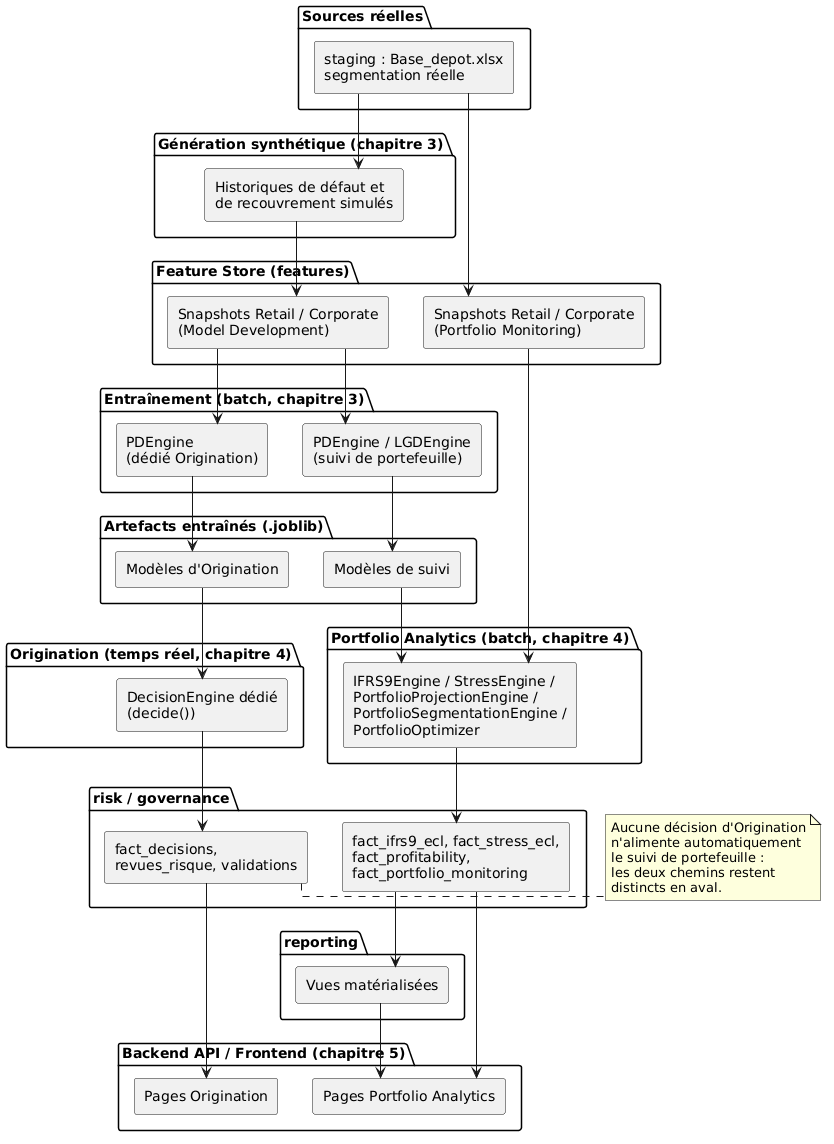
\includegraphics[width=\textwidth,height=0.85\textheight,keepaspectratio]{figures/flux_donnees_global.png}
    \caption{Flux de données global de la plateforme (élaboration personnelle).}
    \label{fig:flux-donnees}
\end{figure}

\section{Architecture logique}

La figure~\ref{fig:architecture-logique} présente l'organisation fonctionnelle de la plateforme, indépendamment de sa réalisation technique.

\begin{figure}[htbp]
    \centering
    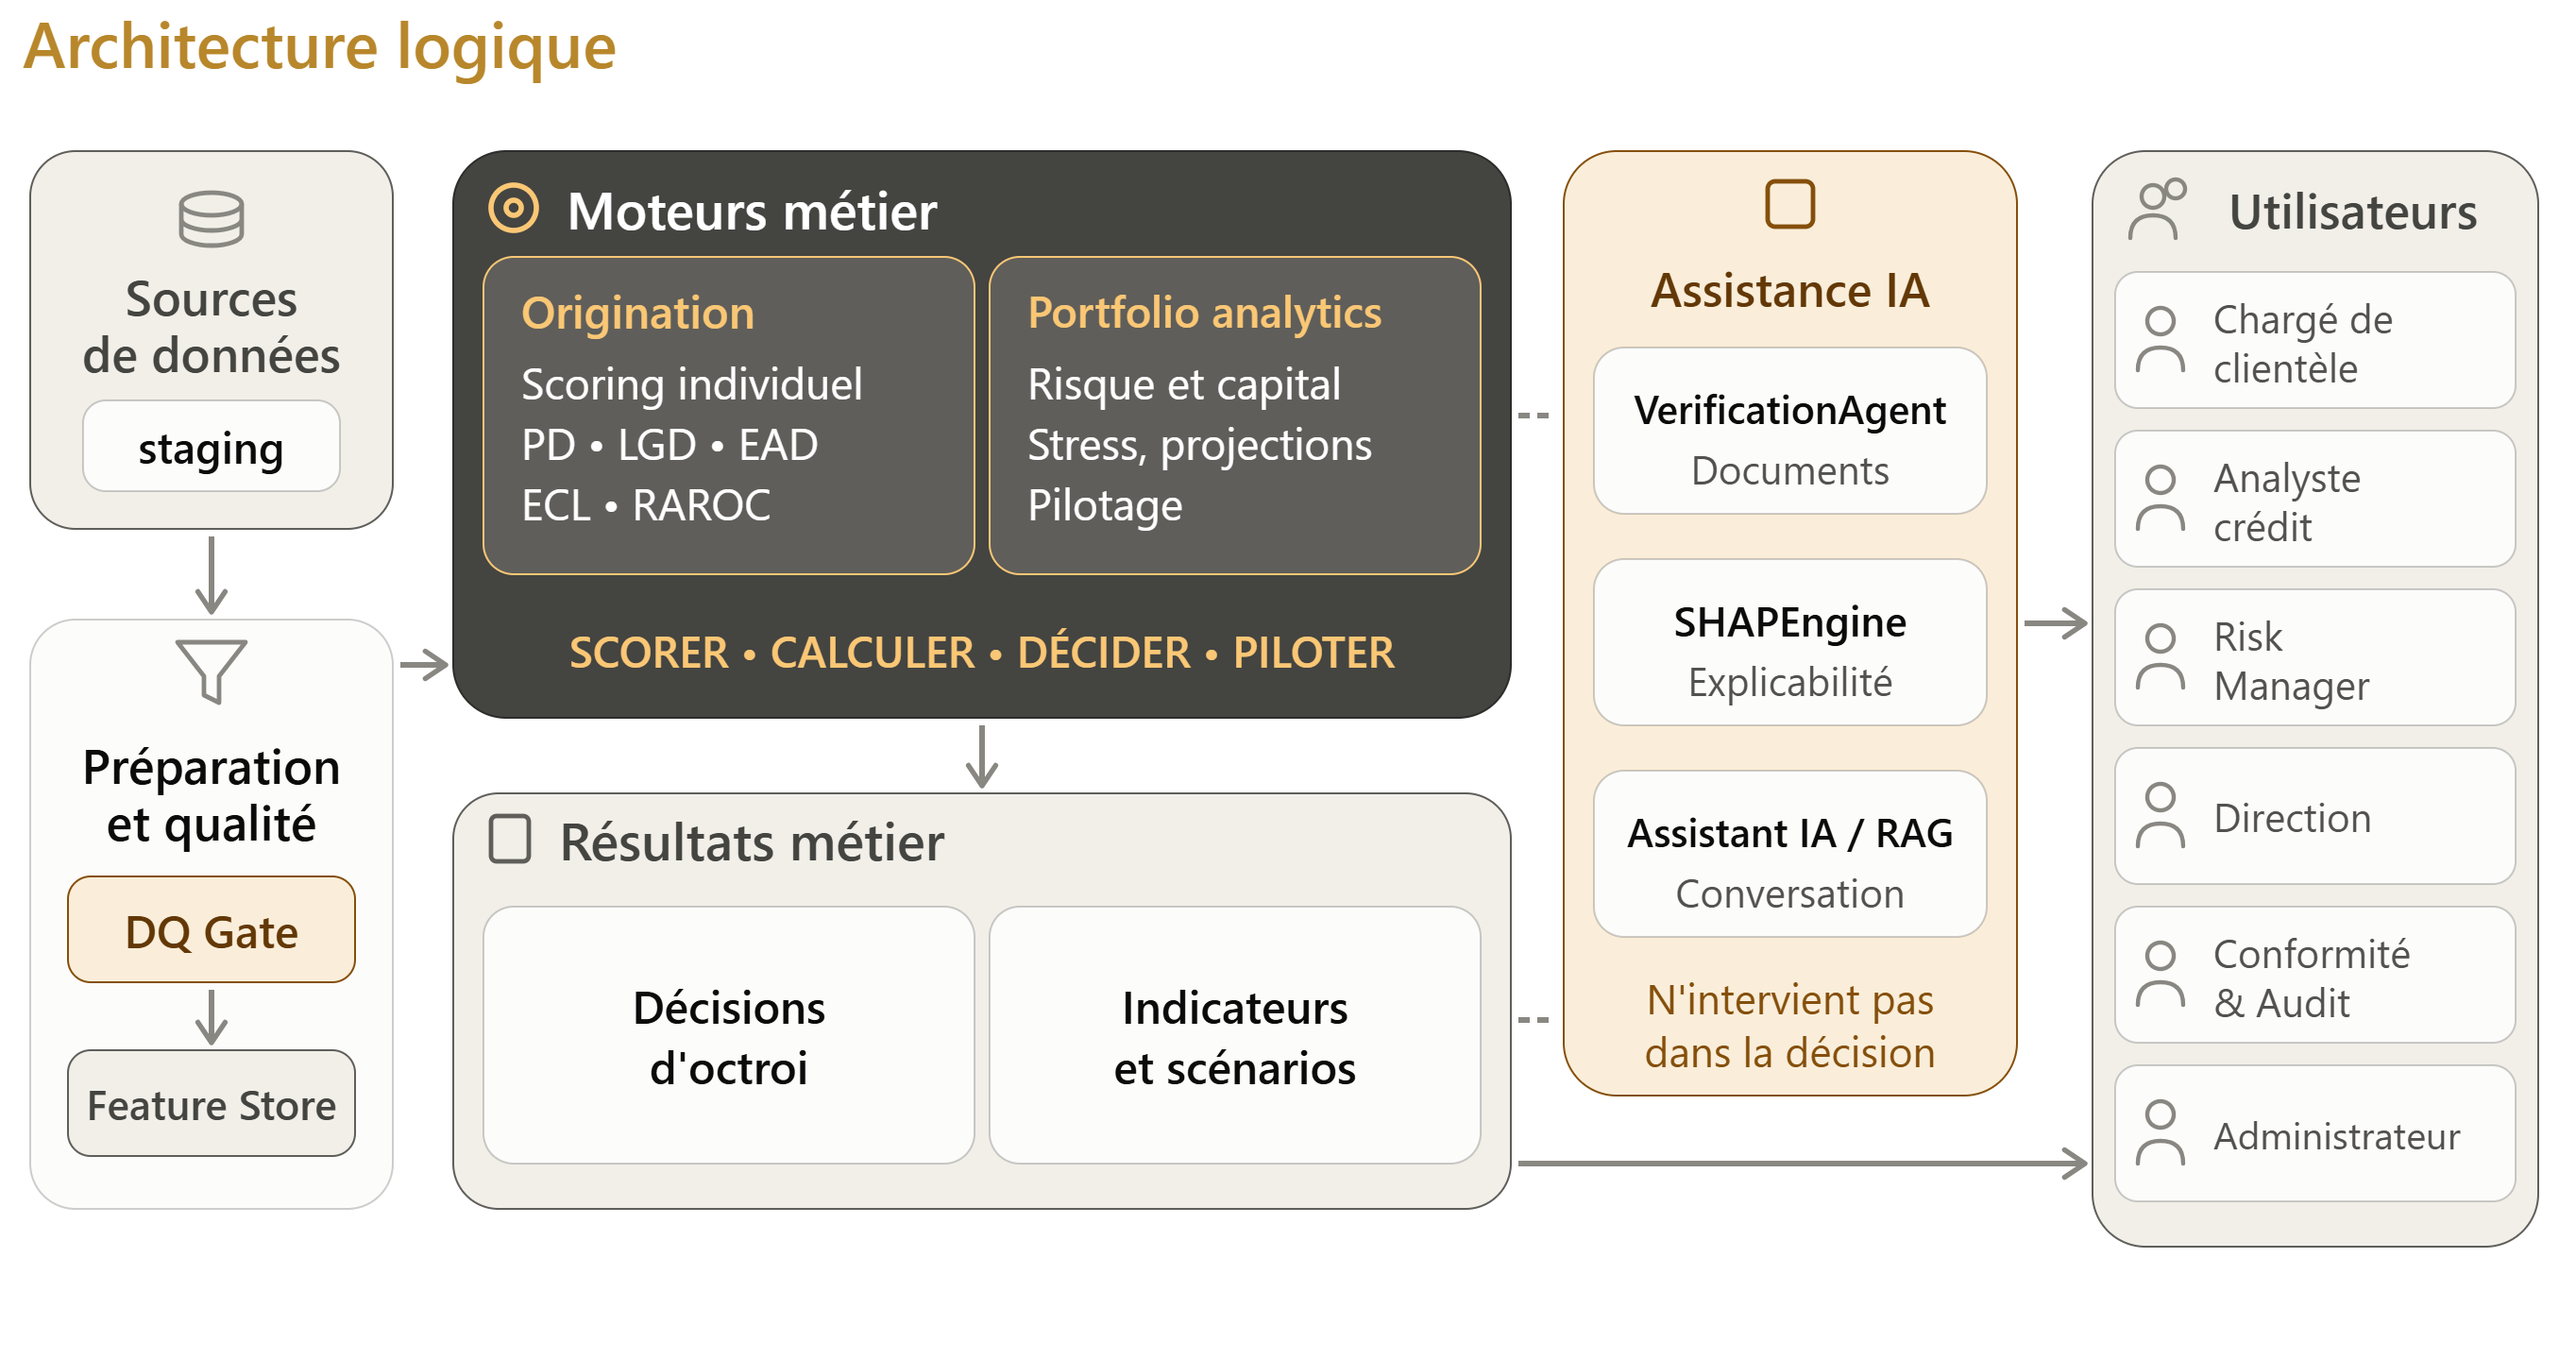
\includegraphics[width=\textwidth]{figures/architecture_logique.png}
    \caption{Architecture logique de la plateforme (élaboration personnelle).}
    \label{fig:architecture-logique}
\end{figure}

Les données réelles entrantes, principalement constituées des informations relatives aux clients et à leurs comptes, sont issues du schéma \texttt{staging} présenté au chapitre 3. Elles sont complétées, dans le cadre du projet, par les historiques de crédit et de remboursement synthétiques construits pour les besoins de la modélisation, également présentés au chapitre 3. L'ensemble est d'abord soumis à une étape de préparation et de qualité : un contrôle de qualité des données, une transformation, puis une construction du Feature Store qui alimente la modélisation.

Les moteurs métier exploitent les données préparées selon les besoins propres à chacun des deux volets déjà distingués au chapitre 1, plutôt qu'une alimentation identique. Pour le suivi de portefeuille, le Feature Store ci-dessus alimente les traitements batch et les modèles entraînés à partir des historiques disponibles : le parcours Portfolio Analytics mobilise ces données et ces modèles pour produire les indicateurs de risque, les pertes attendues, le capital économique et les mesures de rentabilité présentés aux chapitres 3 et 4. Pour l'Origination, les caractéristiques nécessaires à l'évaluation d'un dossier sont constituées séparément, à partir des informations du dossier et de l'historique client exploitable, pour alimenter une évaluation individuelle, probabilité de défaut, perte en cas de défaut, exposition au défaut, perte attendue et capital forfaitaire, rentabilité, puis les règles de décision présentées en section~4.5. Ces traitements produisent des résultats distincts selon le volet : une recommandation d'octroi, éventuellement assortie de conditions ou orientée vers une revue manuelle, accompagnée de son explication pour l'Origination ; des snapshots de risque, des indicateurs et des scénarios, des résultats de pilotage pour le suivi de portefeuille.

Des mécanismes d'explicabilité et de contrôle complètent ces traitements métier sans s'y substituer : l'interprétabilité SHAP contribue à l'explication des résultats de l'Origination, tandis que la vérification documentaire et l'orientation vers une revue humaine apportent des contrôles complémentaires au même parcours. L'assistant conversationnel, présenté en section~5.5, constitue pour sa part une couche consultative transversale : il permet aux utilisateurs d'interroger les données et les services de la plateforme, sans jamais intervenir dans une décision de crédit. Enfin, l'accès à ces résultats est soumis au contrôle d'accès par rôle présenté au chapitre 2, chaque acteur de la plateforme, chargé de clientèle, analyste crédit, Risk Manager, Direction, Conformité et Audit, Administrateur, ne consultant que ce que ses droits lui permettent.

\section{Architecture physique}

La figure~\ref{fig:architecture-physique} détaille la réalisation technique de cette organisation logique, dans l'environnement de développement local du projet.

\begin{figure}[htbp]
    \centering
    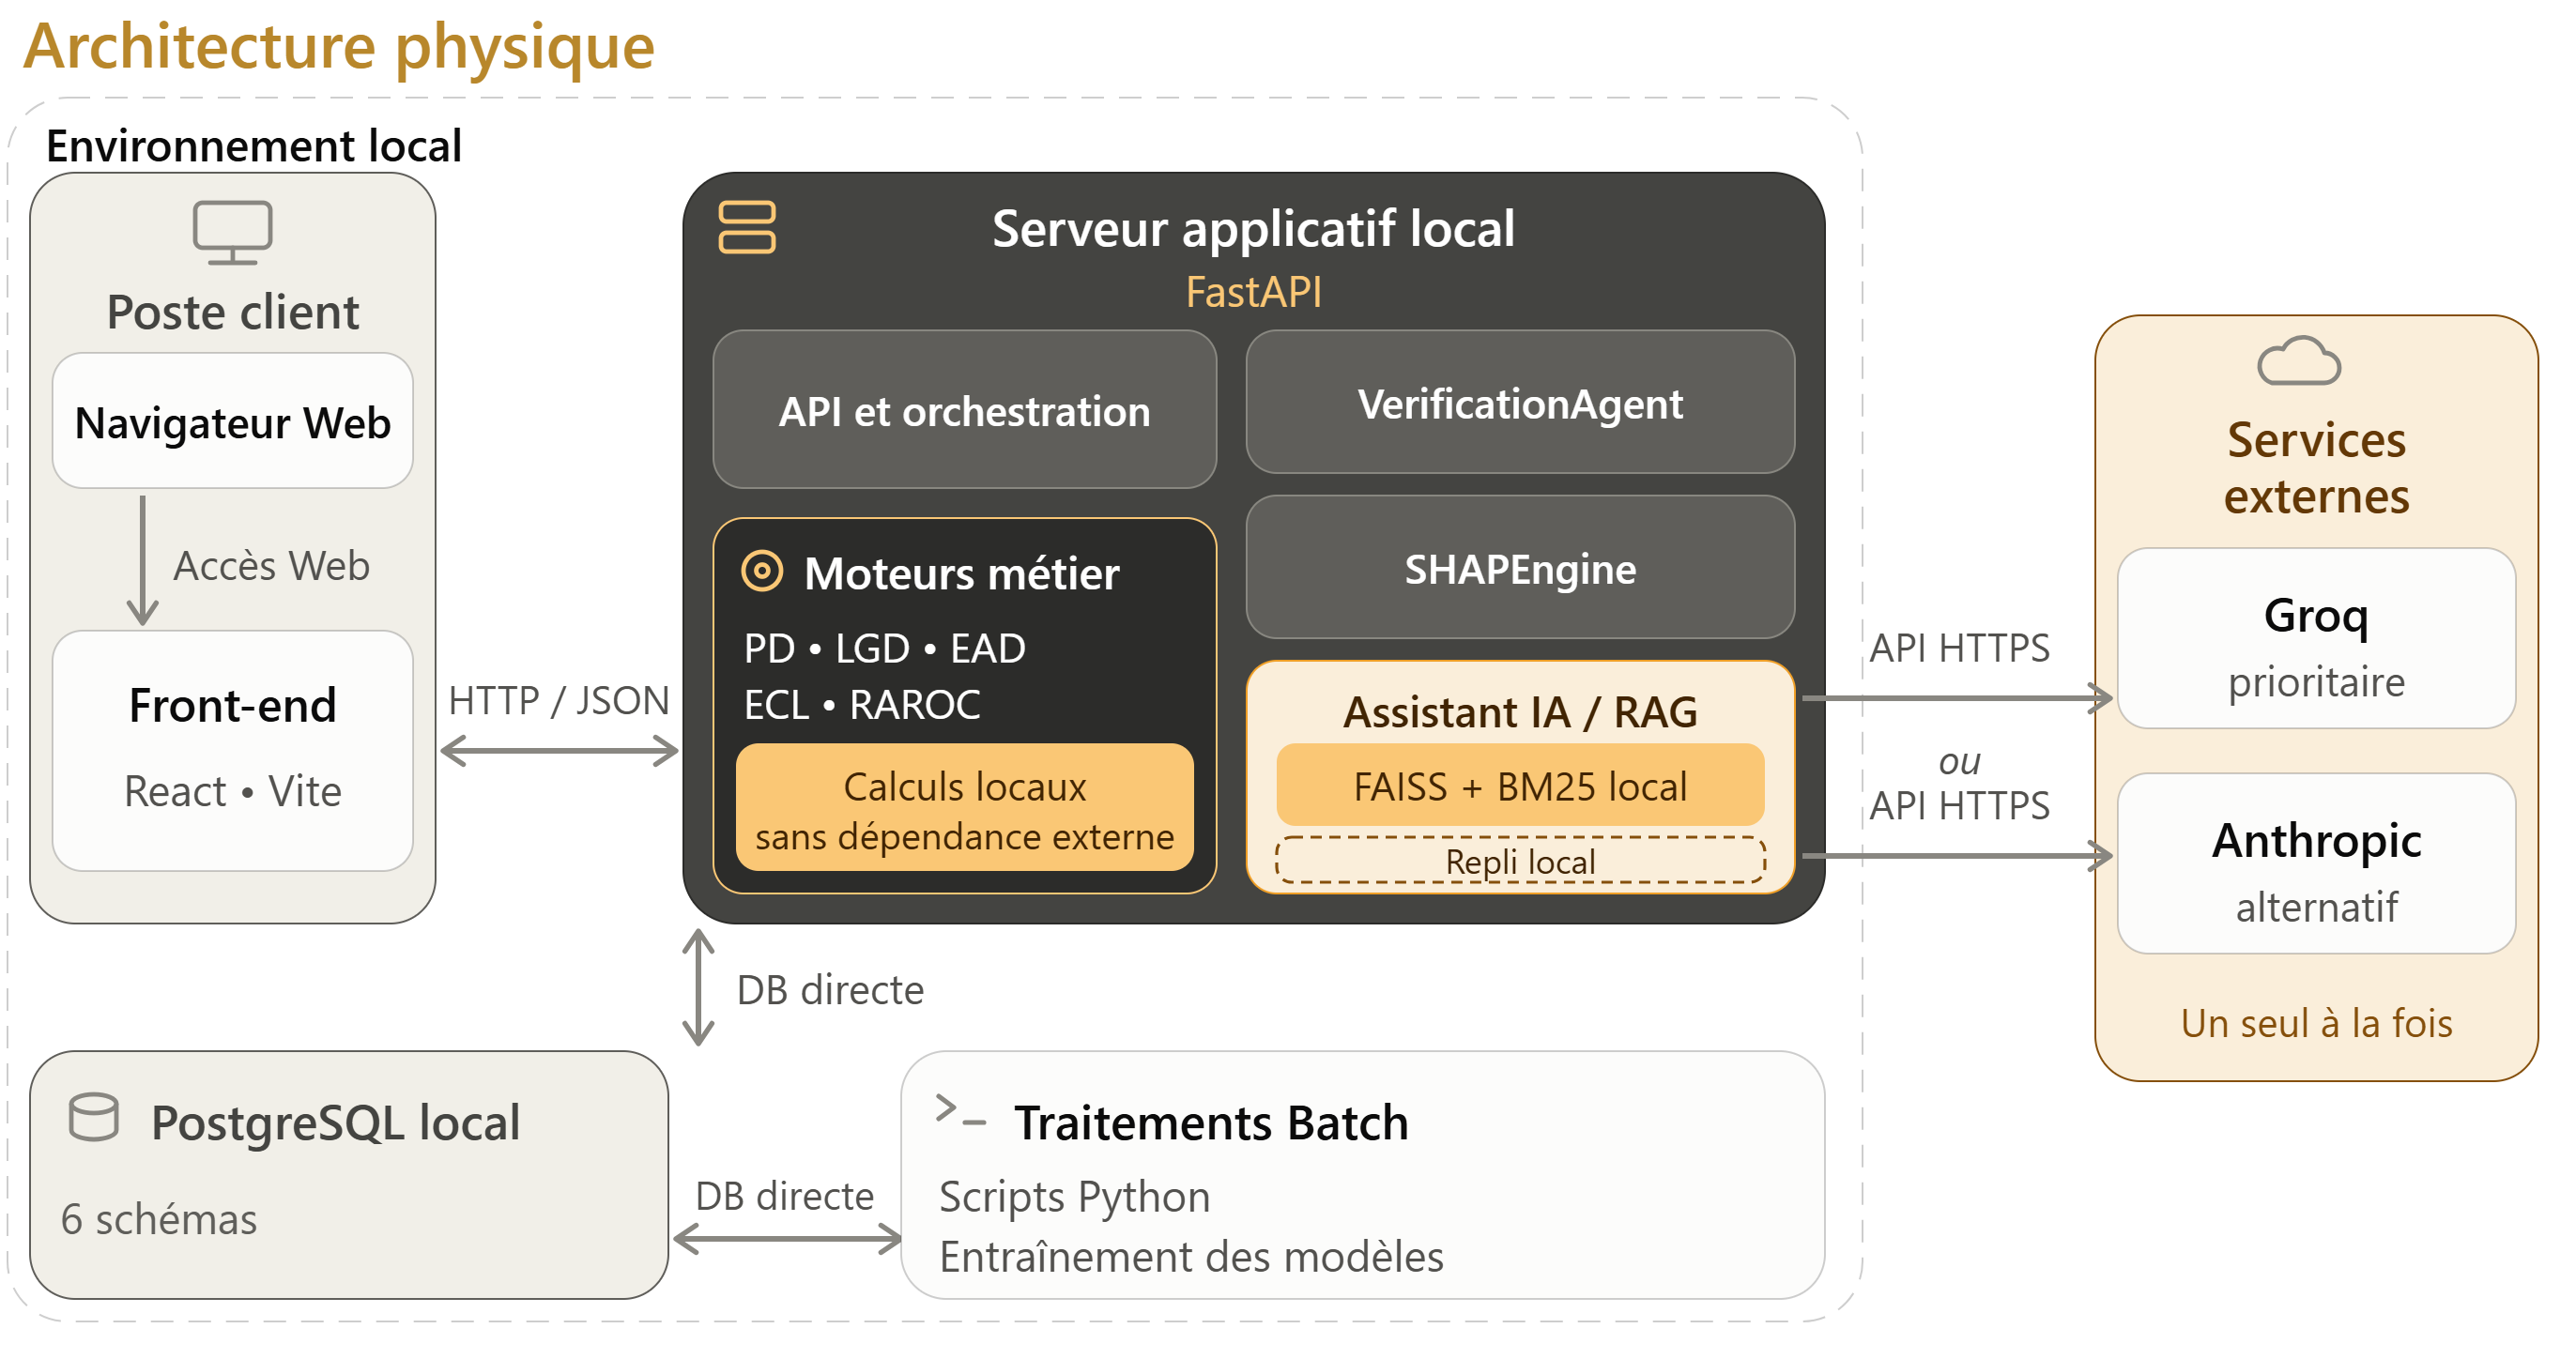
\includegraphics[width=\textwidth]{figures/architecture_physique.png}
    \caption{Architecture physique de la plateforme (élaboration personnelle).}
    \label{fig:architecture-physique}
\end{figure}

Le poste client accède à la plateforme par un navigateur web, qui charge une application front-end développée en React (version 18.3.1) à l'aide de l'outil de développement Vite (version 5.4), servie localement sur le port 5173. Cette application communique avec le serveur applicatif par des requêtes HTTP/JSON, relayées vers le port 8000 par un mécanisme de proxy.

Le serveur applicatif local, un backend FastAPI exécuté par le serveur Uvicorn, regroupe plusieurs composants. Les routes de l'API, les services métier et l'authentification par rôle orchestrent les traitements. Les moteurs de calcul du risque, de rentabilité et de décision, présentés aux chapitres 3 et 4, probabilité de défaut, perte en cas de défaut, exposition au défaut, perte attendue, rentabilité et moteur de décision, s'exécutent localement, sans dépendance à un service externe. Un pipeline d'extraction documentaire, pour l'OCR des documents soumis lors d'une demande, ainsi que le moteur d'interprétabilité SHAP, complètent ce serveur. L'assistant conversationnel, détaillé en section~5.5, s'appuie sur une recherche hybride locale, combinant un index FAISS chargé en mémoire et une recherche lexicale BM25, avant de faire appel à un fournisseur externe de génération de texte : Groq en priorité, ou Anthropic lorsque Groq n'est pas disponible à l'initialisation, un seul des deux étant utilisé à la fois selon cette disponibilité, avec un repli local déterministe si aucun des deux n'est disponible.

Le serveur applicatif et les traitements batch, des scripts Python mobilisant les bibliothèques scikit-learn, XGBoost, LightGBM, SHAP et Optuna déjà présentées au chapitre 3, se connectent tous deux directement à la même base PostgreSQL locale, organisée selon les schémas présentés en section~5.1.

\section{Conception du système et diagrammes UML}

\subsection{Diagramme de séquence du parcours Origination}

La figure~\ref{fig:sequence-origination} détaille, sous la forme d'un diagramme de séquence, l'enchaînement réel des appels pour une demande de crédit, de sa création à sa décision, en deux étapes distinctes.

\begin{figure}[htbp]
    \centering
    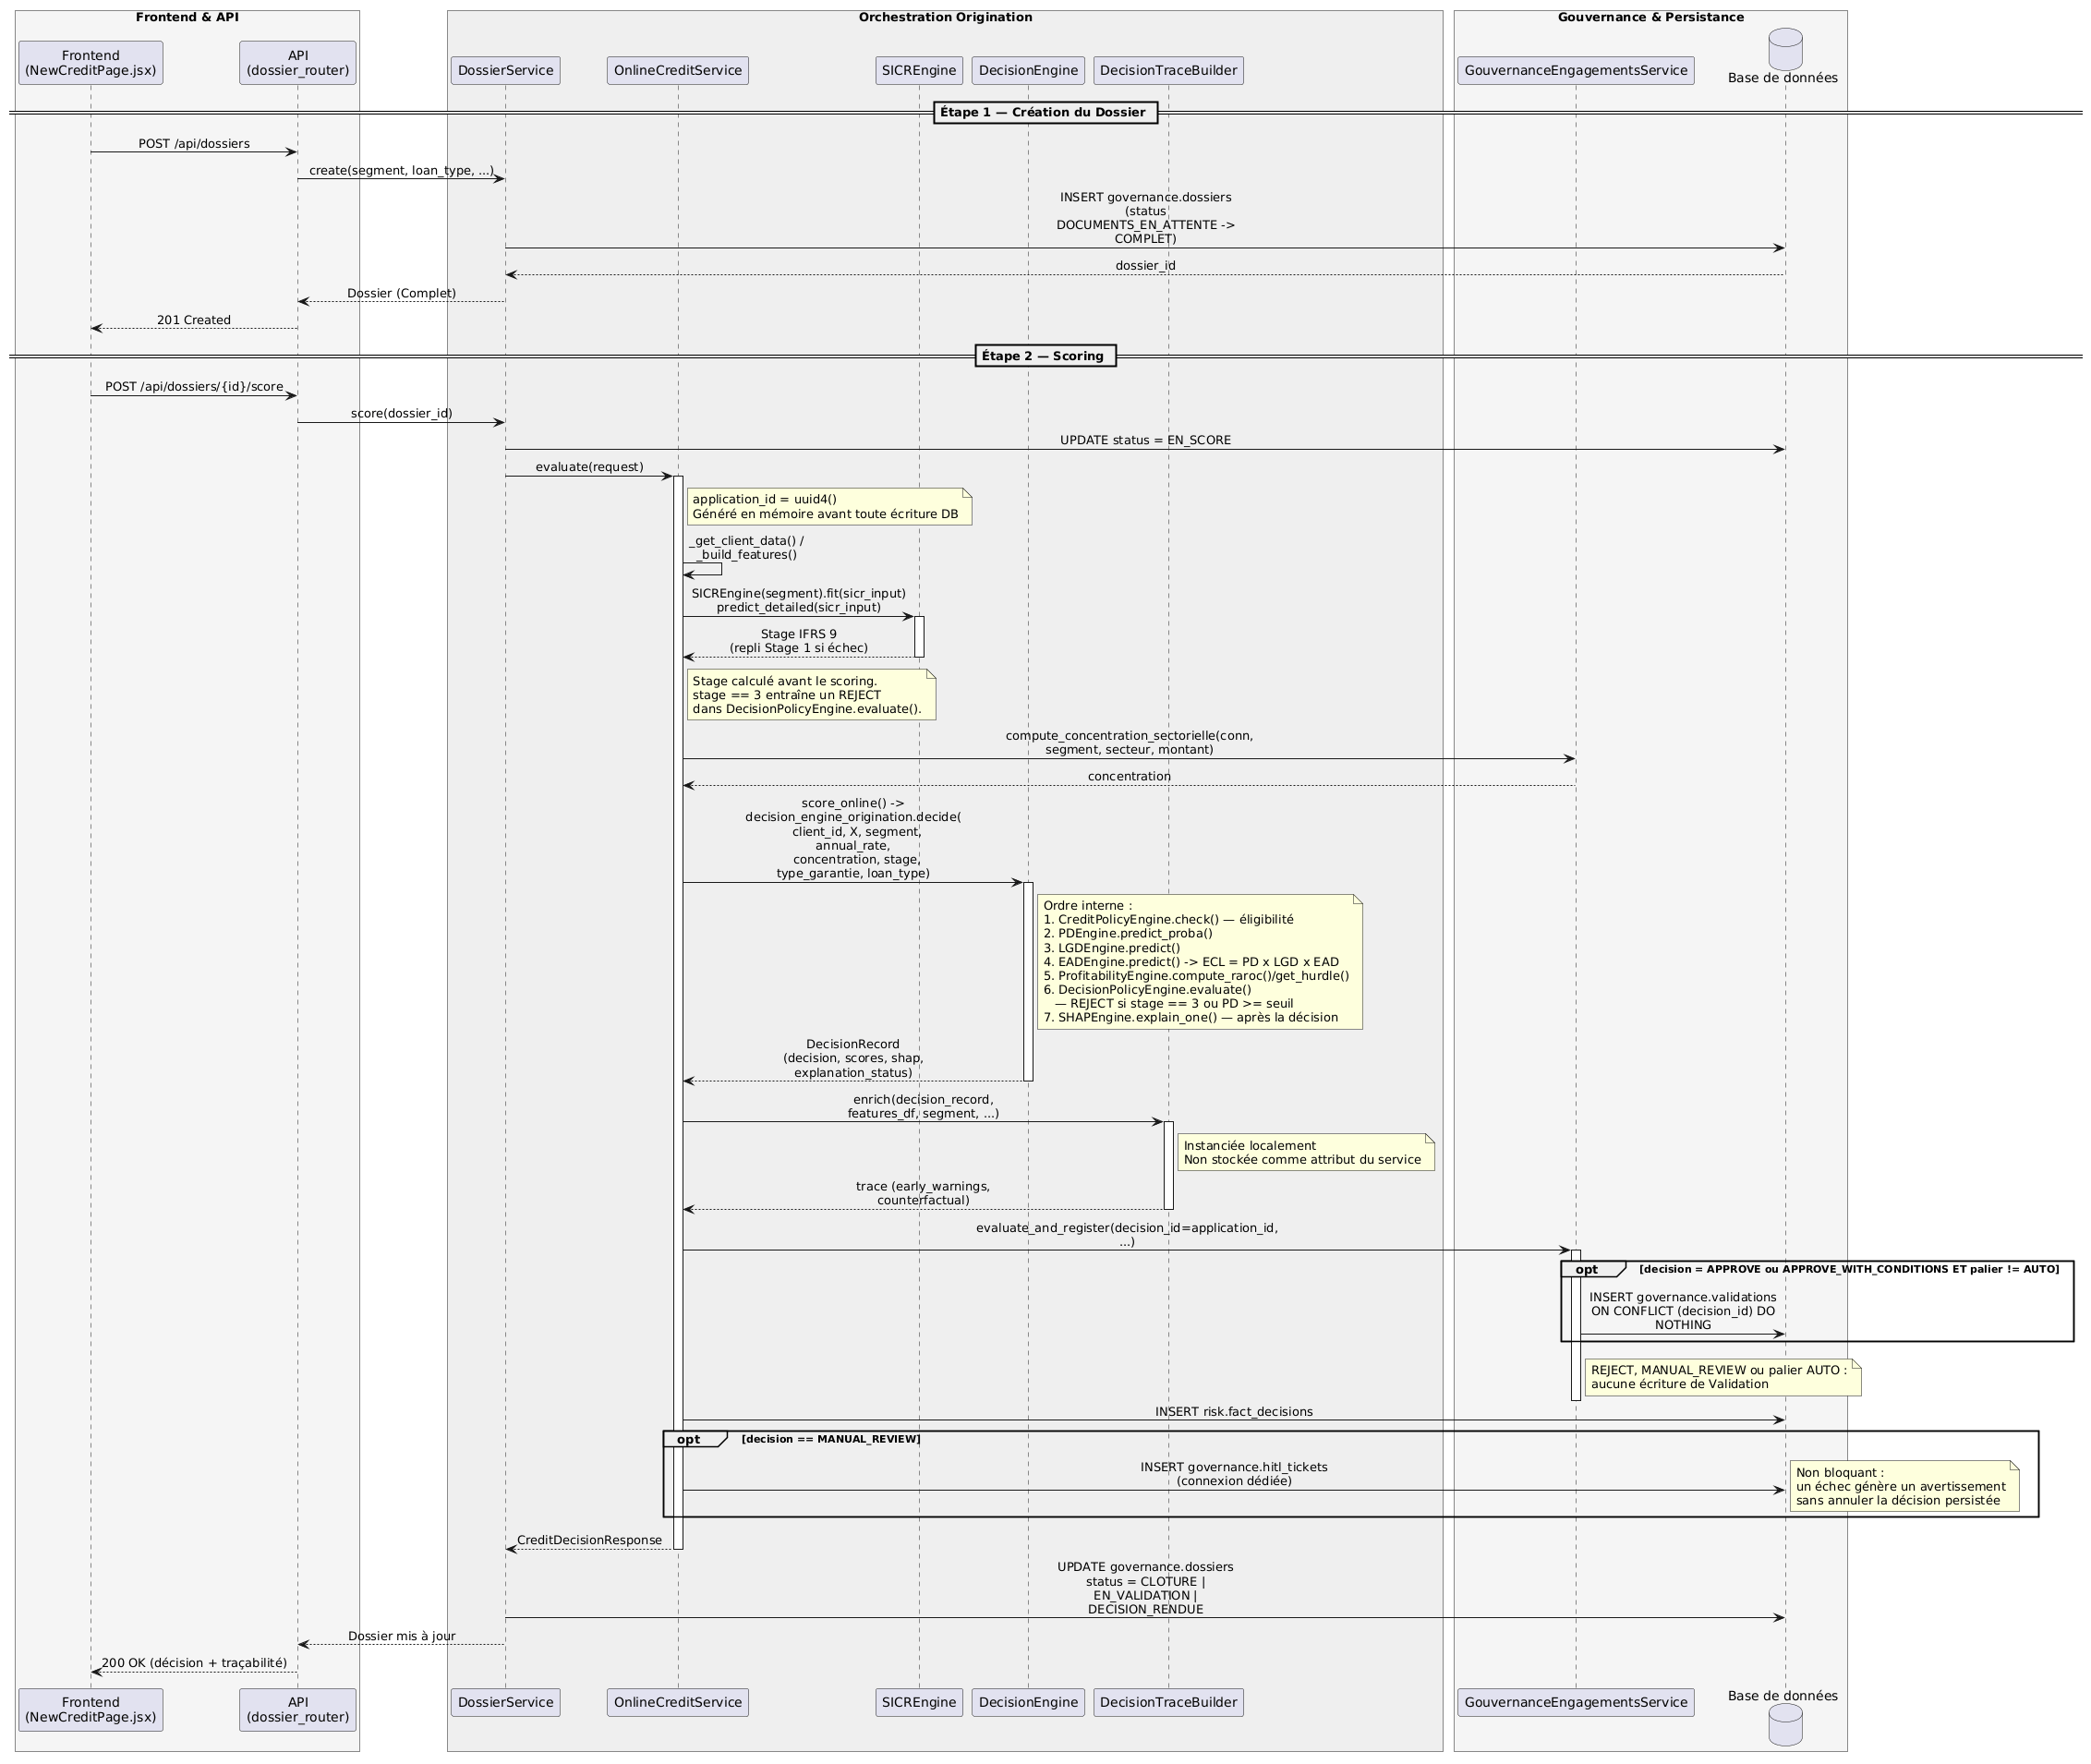
\includegraphics[width=\textwidth]{figures/sequence_origination.png}
    \caption{Diagramme de séquence du parcours Origination (élaboration personnelle).}
    \label{fig:sequence-origination}
\end{figure}

La création du dossier enregistre la demande dans le schéma de gouvernance, dans un statut initial qui évolue une fois les données nécessaires réunies. Le scoring, déclenché séparément, délègue l'ensemble du calcul métier à un point d'entrée unique : un identifiant d'application (\texttt{application\_id}) est généré en mémoire avant la persistance des résultats du scoring, puis le stage IFRS 9 du client est déterminé en amont du scoring, selon les mêmes règles SICR que celles présentées en section~4.2. Ce stage intervient dans l'appréciation de la situation du dossier et dans les règles de décision, sans modifier le calcul simplifié de l'ECL utilisé dans ce parcours, qui repose, pour rappel, sur une probabilité de défaut à douze mois. Le moteur de décision dédié à l'Origination, présenté en section~4.5, est alors invoqué selon l'enchaînement déjà détaillé : éligibilité, probabilité de défaut, perte en cas de défaut, exposition et perte attendue, rentabilité, règles de décision, puis explication SHAP. La décision obtenue est enrichie d'éléments de traçabilité complémentaires, construits à la demande plutôt que conservés en mémoire d'un appel à l'autre, puis soumise à la gouvernance des engagements : une validation humaine n'est enregistrée que si la décision le justifie et que le palier de délégation applicable l'exige, les autres cas n'entraînant aucune écriture à ce titre. Une décision orientée vers une revue manuelle crée, en complément, un ticket dans la file de travail des analystes, sans jamais faire échouer la réponse si cette création rencontre un problème. Le dossier est enfin mis à jour dans un statut qui reflète l'issue de ce traitement.

\subsection{Diagramme de séquence du traitement batch du portefeuille}

La figure~\ref{fig:sequence-monitoring} détaille, sous la forme d'un diagramme de séquence, l'enchaînement réel du traitement batch qui produit un instantané du suivi de portefeuille, pour un mois d'activité donné.

\begin{figure}[htbp]
    \centering
    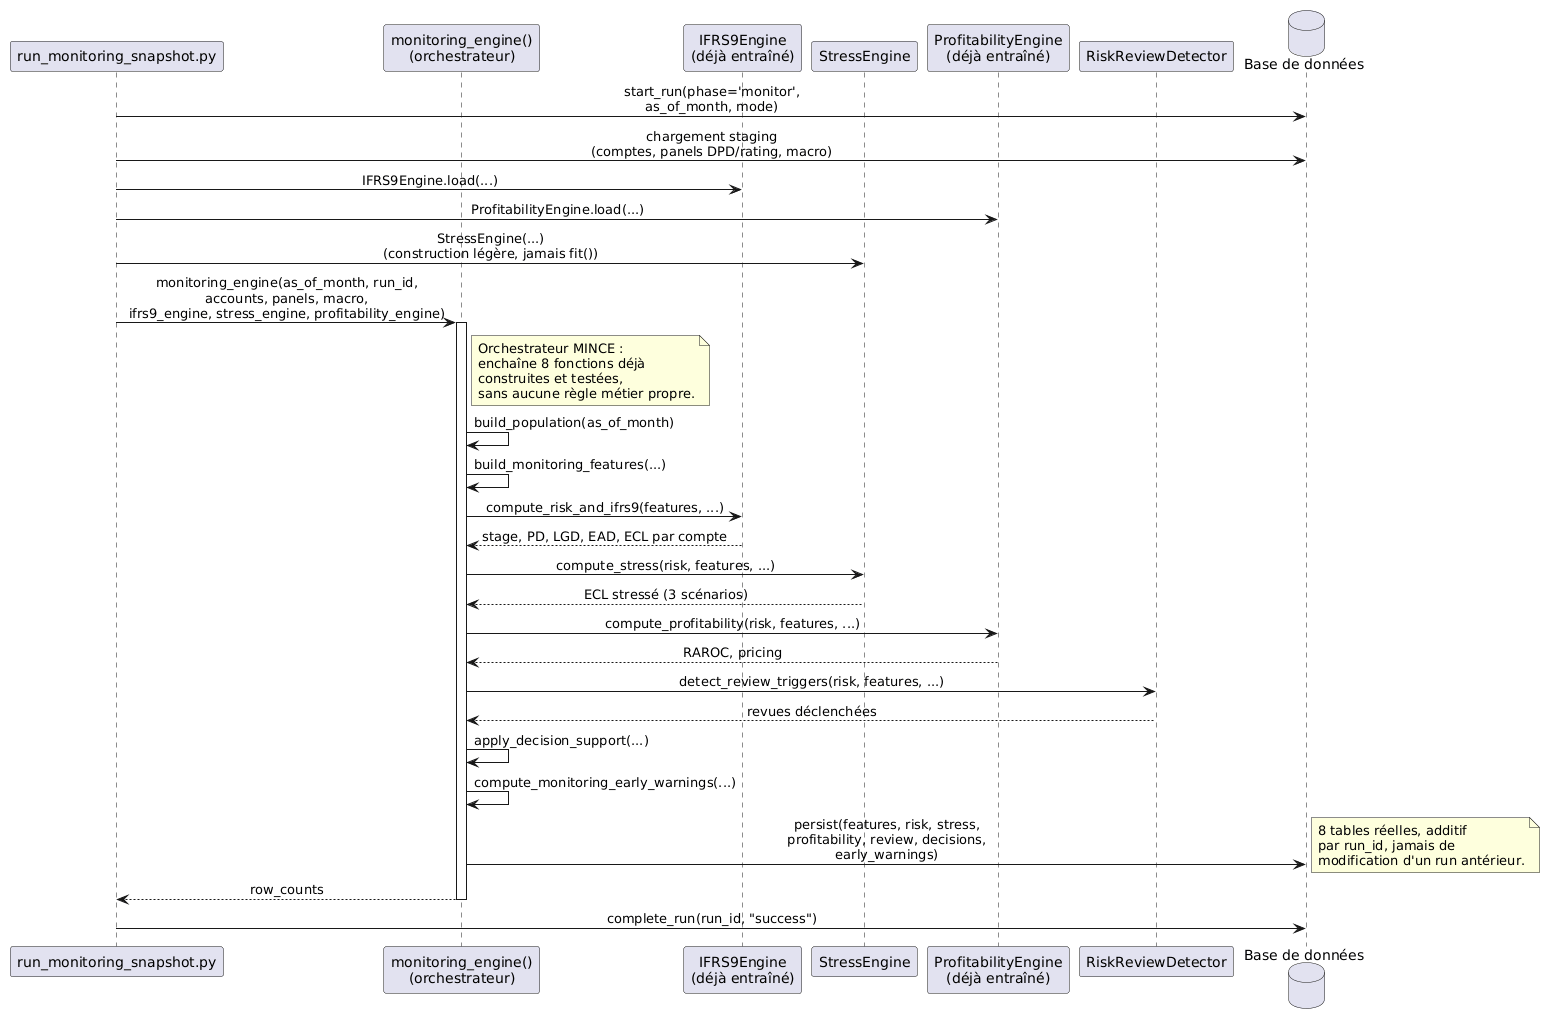
\includegraphics[width=\textwidth]{figures/sequence_monitoring_batch.png}
    \caption{Diagramme de séquence du traitement batch du portefeuille (élaboration personnelle).}
    \label{fig:sequence-monitoring}
\end{figure}

Ce traitement charge d'abord les modèles déjà entraînés, présentés au chapitre 3, ainsi que les données réelles du portefeuille à la date considérée, avant de déléguer l'ensemble du calcul à un orchestrateur unique. Celui-ci enchaîne, dans un ordre fixe, huit étapes déjà construites indépendamment les unes des autres, sans ajouter de règle métier qui lui serait propre : la construction de la population de comptes concernés, la construction des caractéristiques nécessaires, le calcul du risque et des pertes attendues selon IFRS 9, le calcul des indicateurs sous stress, le calcul de la rentabilité, la détection des comptes nécessitant une revue, l'application des règles de suivi du portefeuille, distinctes du moteur de décision d'Origination présenté ci-dessus, puis le calcul de signaux de vigilance complémentaires. Le résultat de ces huit étapes est enfin persisté dans les tables réelles du suivi de portefeuille, de façon additive par exécution, sans jamais modifier une exécution antérieure.

\subsection{Diagramme d'activité du processus de décision}

La figure~\ref{fig:activite-decision} représente, sous la forme d'un diagramme d'activité, l'enchaînement des règles hiérarchiques présentées en section~4.5, depuis la vérification de l'éligibilité jusqu'à l'une des quatre catégories de décision possibles.

\begin{figure}[htbp]
    \centering
    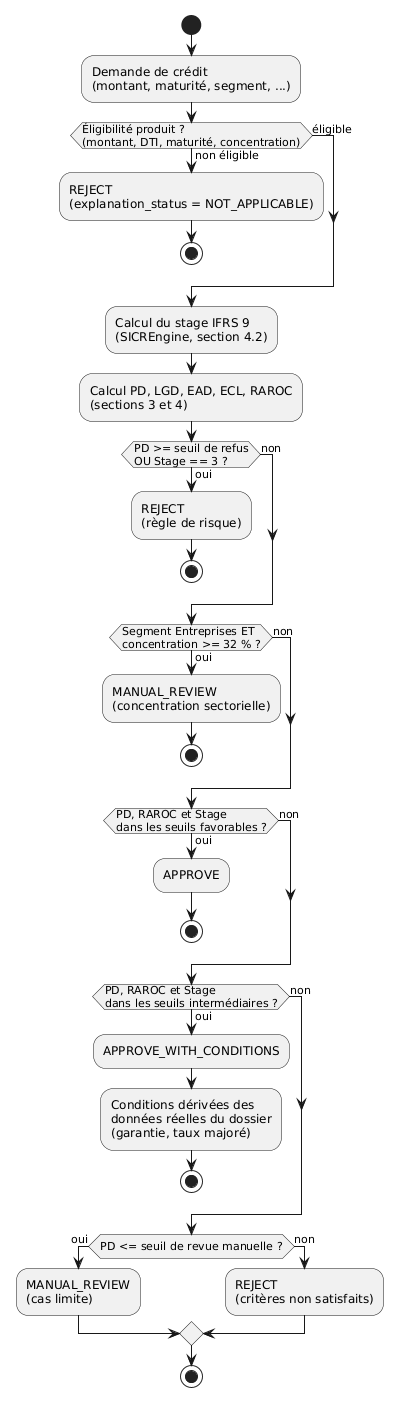
\includegraphics[width=\textwidth,height=0.85\textheight,keepaspectratio]{figures/activite_decision_origination.png}
    \caption{Diagramme d'activité du processus de décision Origination (élaboration personnelle).}
    \label{fig:activite-decision}
\end{figure}

Ce diagramme met en évidence deux propriétés déjà soulignées au chapitre 4 : l'éligibilité est vérifiée avant tout calcul de risque, de sorte qu'un refus à ce stade n'engage jamais les modèles prédictifs ; et les règles de décision proprement dites s'appliquent ensuite dans un ordre strictement hiérarchique, un refus fondé sur le risque ou le stage prévalant sur toute autre règle, jusqu'au cas limite qui bascule vers une revue manuelle plutôt que vers un refus automatique.

\subsection{Diagramme de classes}

La figure~\ref{fig:diagramme-classes} présente l'organisation des classes qui implémentent les moteurs métier et leur orchestration.

\begin{figure}[htbp]
    \centering
    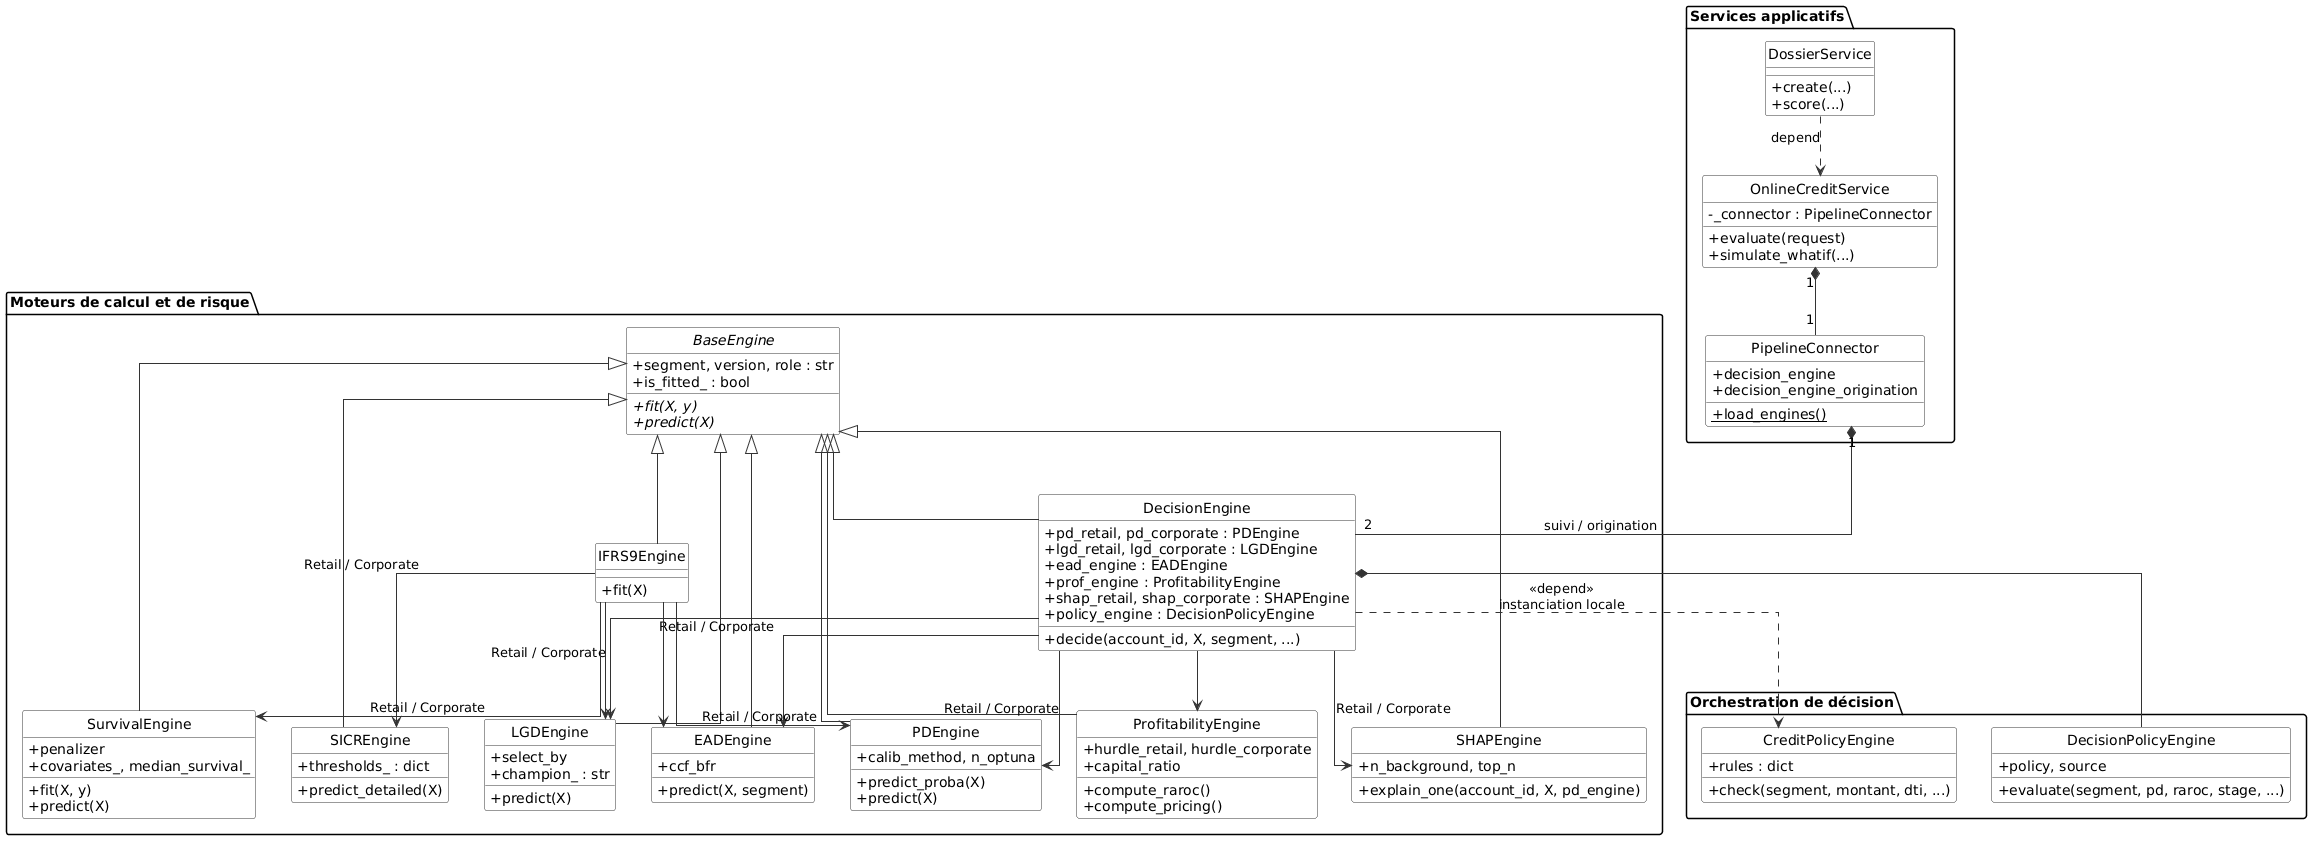
\includegraphics[width=\textwidth]{figures/diagramme_classes.png}
    \caption{Diagramme de classes des moteurs de calcul et de décision (élaboration personnelle).}
    \label{fig:diagramme-classes}
\end{figure}

L'ensemble des moteurs de risque présentés aux chapitres 3 et 4, probabilité de défaut, perte en cas de défaut, exposition au défaut, détection de dégradation du risque, modèle de survie, rentabilité et interprétabilité SHAP, hérite d'une classe commune qui définit leur interface : des attributs partagés (segment, version, rôle), un indicateur d'état entraîné, et deux méthodes de même signature, l'une pour la préparation du moteur, l'autre pour le calcul de sa sortie. Cette interface commune ne signifie pas que chaque moteur apprend statistiquement à partir de données : pour l'exposition au défaut ou la détection de dégradation du risque, présentées comme des formules déterministes aux chapitres 3 et 4, la méthode de préparation ne fait que valider les données attendues, sans ajustement de paramètres. Le moteur qui orchestre le calcul des pertes attendues selon IFRS 9, présenté en section~4.2, hérite de cette même classe et compose plusieurs de ces moteurs.

Le moteur de décision, présenté en section~4.5, compose à son tour les moteurs de probabilité de défaut, de perte en cas de défaut, d'exposition au défaut, de rentabilité et d'interprétabilité SHAP, distinctement pour chaque segment, ainsi qu'un moteur de règles de décision et un moteur d'éligibilité, présentés eux aussi en section~4.5. Conformément à la distinction établie en section~5.1, deux instances de ce moteur de décision coexistent, l'une pour le suivi de portefeuille, l'autre dédiée à l'Origination ; le connecteur qui charge les artefacts entraînés en conserve une référence distincte pour chacune, et c'est exclusivement celle dédiée à l'Origination que mobilise le service de crédit en ligne, lui-même sollicité par le service de gestion des dossiers présenté dans le diagramme de séquence précédent.

\section{Architecture de l'assistant IA}

L'assistant conversationnel déjà introduit en section~5.1 interroge les données et résultats déjà produits par la plateforme, sans jamais calculer lui-même un indicateur de risque ni intervenir dans une décision de crédit ; cette limite est imposée dans le code, par un message rappelé à chaque réponse, et non seulement documentée. Son architecture s'organise en plusieurs étapes.

\begin{figure}[H]
\centering
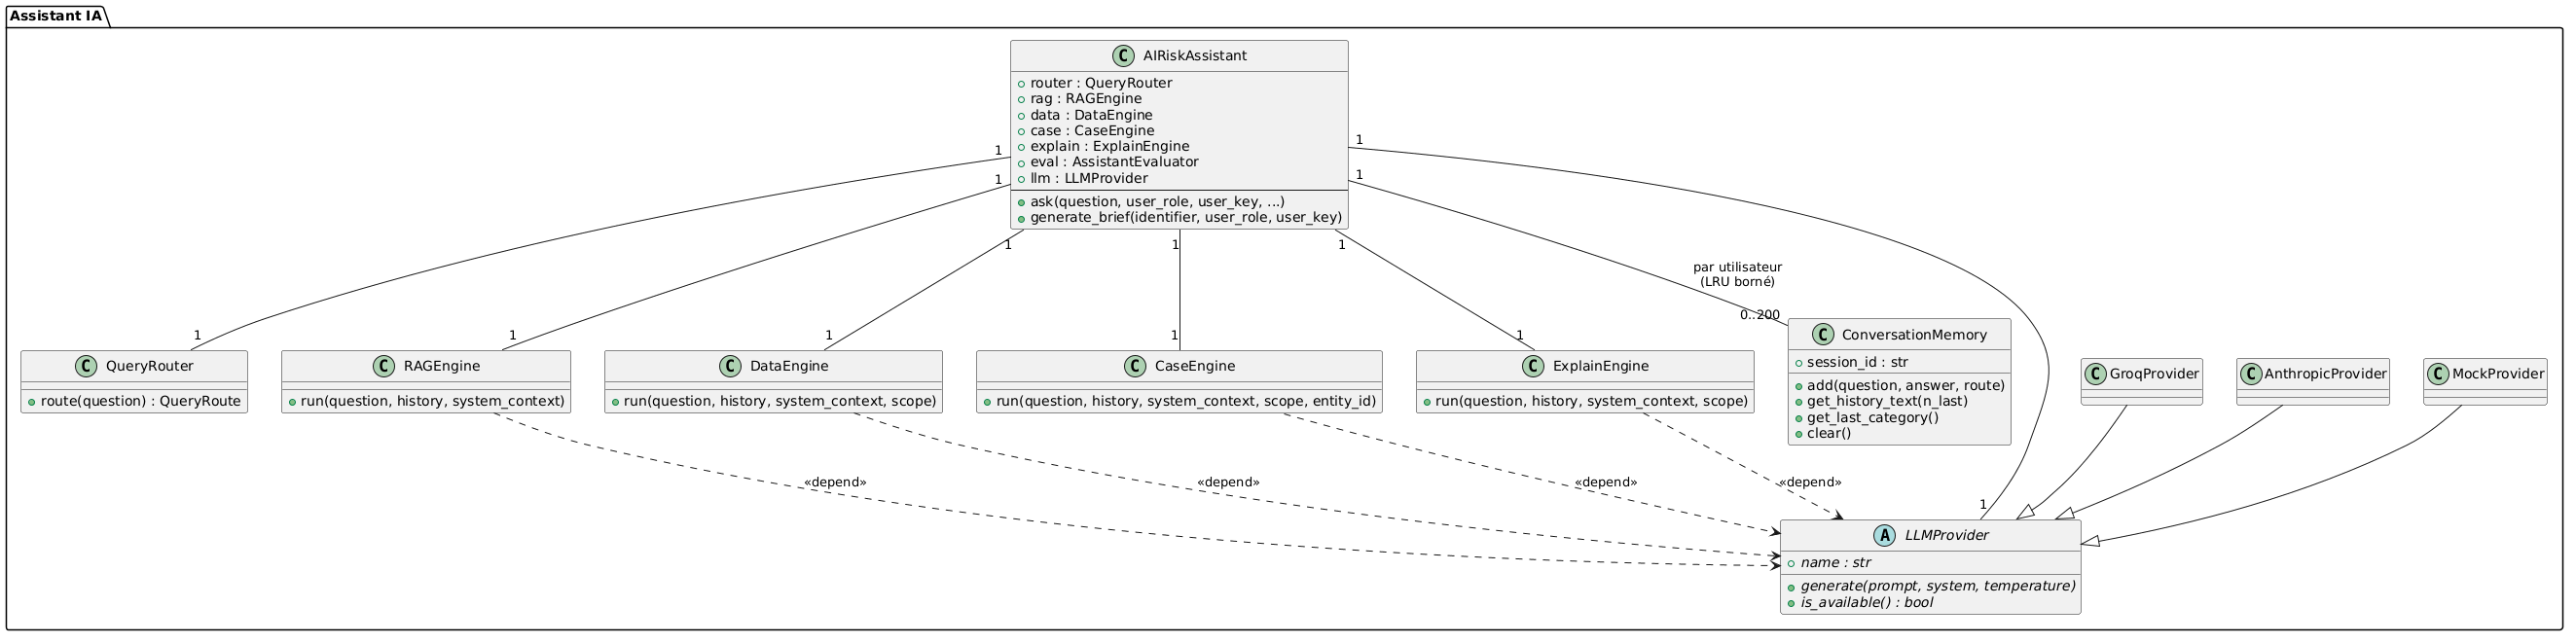
\includegraphics[width=\textwidth]{figures/diagramme_classes_assistant.png}
\caption{Diagramme de classes du sous-système Assistant IA}
\label{fig:diagramme-classes-assistant}
\end{figure}

La figure~\ref{fig:diagramme-classes-assistant} complète le diagramme de classes des moteurs de risque et de l'orchestration de décision présenté en section~5.4 : \texttt{AIRiskAssistant} orchestre un routeur et quatre moteurs spécialisés, partage un même fournisseur de génération de texte, interchangeable sans modifier le code appelant, et gère une mémoire conversationnelle par utilisateur authentifié, bornée par éviction LRU plutôt qu'une instance unique partagée.

Une question posée en langage naturel est d'abord orientée vers l'un de quatre moteurs spécialisés par un routeur à deux niveaux : une première couche de mots-clés traite rapidement les cas évidents, une seconde couche, fondée sur la similarité sémantique entre la question et des exemples de référence, traite les cas plus ambigus. Les questions portant sur la réglementation ou des notions générales (IFRS 9, BCEAO) sont dirigées vers un moteur de recherche documentaire ; celles portant sur le portefeuille, vers un moteur interrogeant directement les résultats déjà calculés ; celles portant sur un dossier client particulier, vers un moteur dédié ; celles portant sur l'interprétation d'un résultat, vers un moteur d'explication s'appuyant sur les valeurs SHAP présentées au chapitre 3.

Le moteur de recherche documentaire repose sur une recherche hybride locale, déjà présentée en section~5.3 : un index FAISS d'embeddings sémantiques, combiné à une recherche lexicale BM25, afin de retrouver les passages pertinents d'une base documentaire réglementaire. Les passages documentaires retrouvés ou les résultats fournis par les moteurs spécialisés constituent le contexte transmis au fournisseur de génération de texte. Celui-ci les exploite pour formuler une réponse en langage naturel, sans se substituer aux moteurs qui produisent les données et les indicateurs.

Le contrôle d'accès par rôle, présenté au chapitre 2, s'applique à deux niveaux distincts avant qu'une donnée n'atteigne ce fournisseur externe. D'abord, à l'intérieur même des moteurs spécialisés, chaque résultat de requête est filtré selon les catégories de données autorisées pour le rôle de l'utilisateur, probabilité de défaut, perte en cas de défaut, exposition, perte attendue, rentabilité, facteurs SHAP, décisions ou revues, un chargé de clientèle n'obtenant par exemple jamais les catégories de risque quantitatif réservées à un analyste crédit ou à un Risk Manager. Un second contrôle, appliqué au texte de contexte assemblé, complète ce filtrage avant la transmission au fournisseur externe. Cette double frontière vise à empêcher qu'une donnée non autorisée pour un rôle n'entre dans le contexte transmis au fournisseur de génération, plutôt que de compter sur ce dernier pour ne pas la restituer.

Une mémoire conversationnelle, propre à chaque utilisateur authentifié, conserve les derniers échanges afin de résoudre les références d'une question à l'autre, par exemple « son RAROC », en référence au dernier client mentionné. Avant sa restitution, chaque réponse fait également l'objet d'une auto-évaluation, un contrôle supplémentaire sur la réponse produite, qui ne constitue ni une validation humaine ni une preuve de son exactitude. Enfin, les échanges sont soumis à une double traçabilité : un journal propre à l'assistant et le journal d'audit chaîné de la plateforme, présenté au chapitre 2.

\begin{figure}[H]
\centering
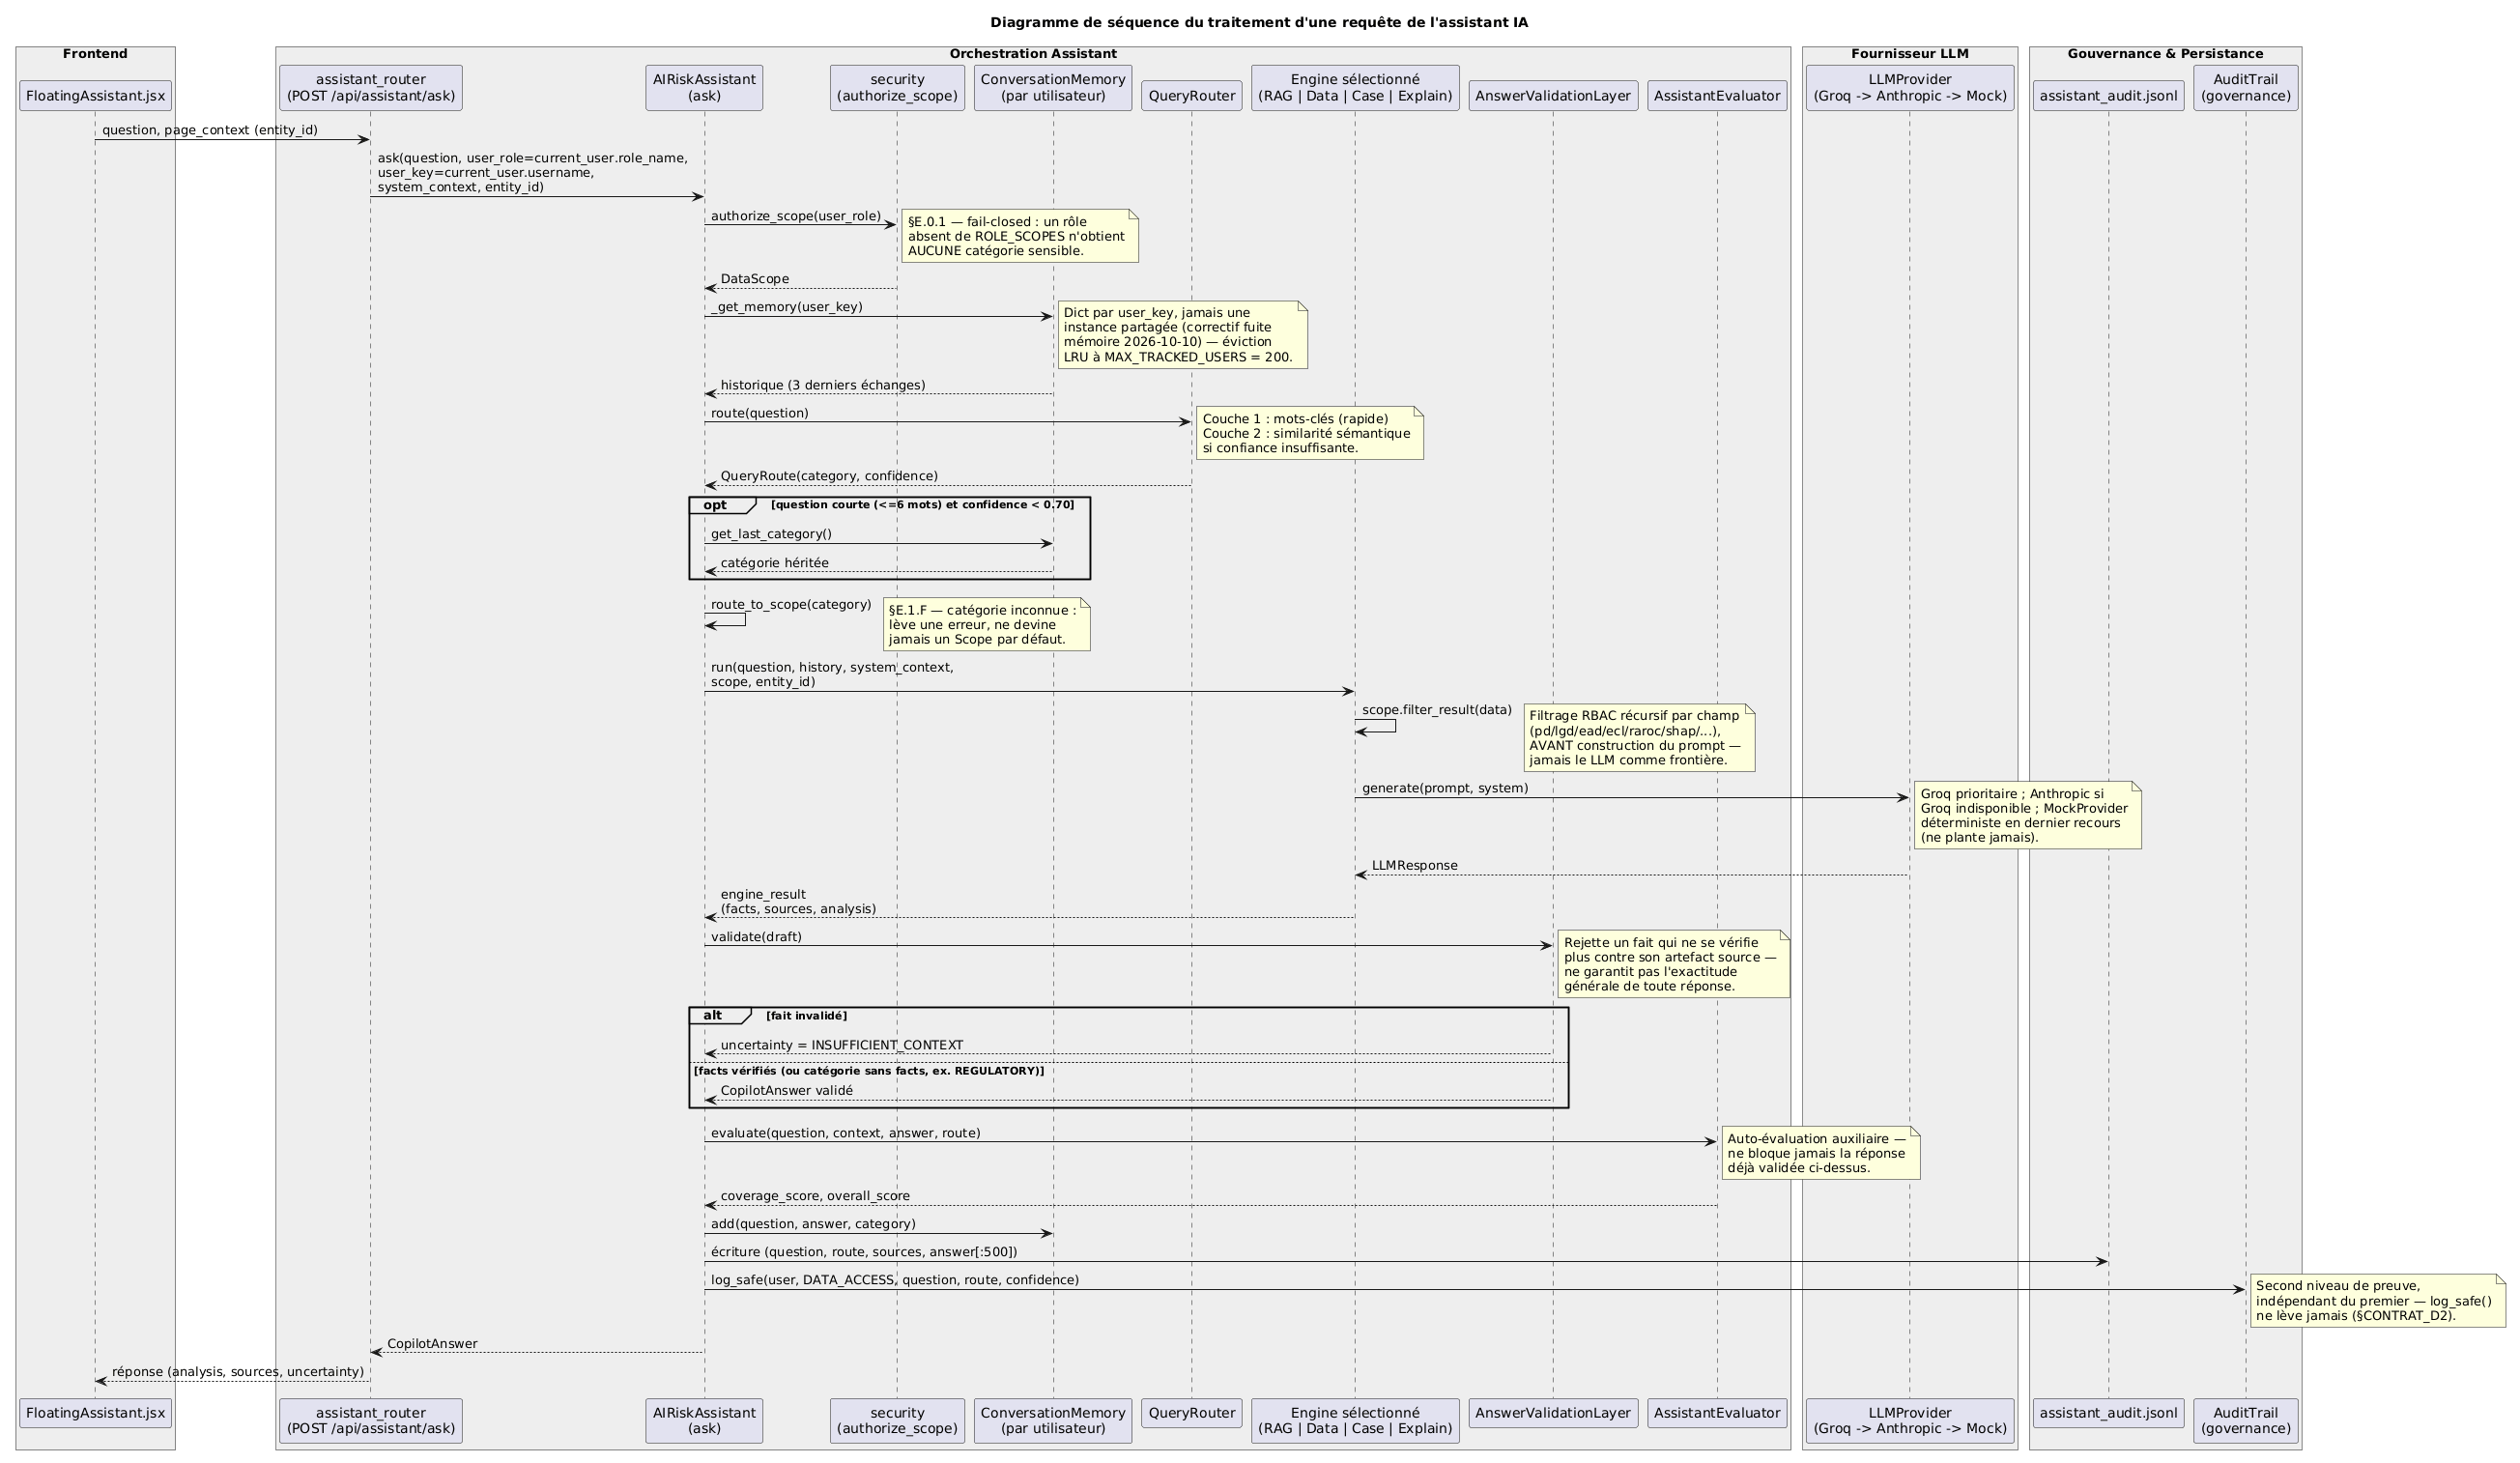
\includegraphics[width=\textwidth]{figures/sequence_assistant.png}
\caption{Diagramme de séquence du traitement d'une requête de l'assistant IA}
\label{fig:sequence-assistant}
\end{figure}

La figure~\ref{fig:sequence-assistant} rend explicite l'ordre réel de ces étapes, déjà décrites en prose ci-dessus : le contrôle d'accès par rôle est résolu avant même la mémoire conversationnelle, le routage attribue un \textit{Scope} explicite qui échoue plutôt que de deviner une catégorie par défaut, et le filtrage RBAC s'exécute à la sortie de chaque moteur spécialisé, avant la construction du prompt transmis au fournisseur externe. La couche de validation des réponses rejette un fait qui ne se vérifie plus contre son artefact source, sans garantir pour autant l'exactitude générale de toute réponse produite ; l'auto-évaluation qui suit reste, de la même façon, un contrôle auxiliaire et non une preuve de correction.

\section*{Conclusion du chapitre}

Ce chapitre a présenté l'architecture qui met en œuvre les modèles et les mécanismes décrits aux chapitres 3 et 4. Deux chemins de traitement, l'un batch, l'autre temps réel, coexistent sans dupliquer toute leur logique : plusieurs moteurs de calcul sont réutilisés entre eux, tandis que d'autres composants, modèles entraînés, moteur de décision effectivement exécuté, restent propres à l'un ou à l'autre. Cette organisation logique repose sur une réalisation technique précise, détaillée par les diagrammes d'architecture et les diagrammes UML présentés, et s'accompagne d'un assistant conversationnel qui complète la plateforme sans jamais se substituer à ses mécanismes de décision, ses propres garde-fous d'accès aux données faisant l'objet d'une attention comparable à celle des moteurs de risque. Le chapitre suivant aborde la réalisation effective de cette architecture et sa mise en œuvre, jusqu'à sa validation.

\chapter{Réalisation, validation et mise en œuvre}

Ce dernier chapitre montre comment l'architecture présentée au chapitre précédent a été effectivement construite. Il présente l'environnement technique mobilisé, puis la réalisation des modules de la plateforme et de l'assistant conversationnel, avant de donner à voir cette réalisation du point de vue de l'utilisateur, à travers les interfaces et parcours réellement implémentés. Une campagne de validation confronte ensuite l'ensemble de ces réalisations à une exécution réelle, et un bilan referme ce chapitre en distinguant ce qui a été obtenu de ce qui reste, à ce stade, une limite assumée.

\section{Environnement technique}

\subsection{Environnement de calcul et de modélisation}

\begin{center}
\begin{tcbraster}[raster columns=3, raster equal height]
\techcard{figures/logos/python.svg}{Python}{Langage de programmation}{Environnement principal de développement et d'exécution des traitements de préparation des données, de modélisation du risque et des services métier.}
\techcard{figures/logos/git.svg}{Git}{Gestion de versions}{Suivi de l'évolution du code source, conservation de l'historique des modifications et organisation des changements apportés au projet.}
\techcard{figures/logos/github.svg}{GitHub}{Hébergement du dépôt}{Plateforme d'hébergement du dépôt Git du projet.}
\techcard{figures/logos/pandas.svg}{pandas}{Manipulation des données}{Nettoyage, transformation et préparation des jeux de données exploités par les moteurs de risque, présentés au chapitre 3.}
\techcard{figures/logos/scikitlearn.svg}{scikit-learn}{Apprentissage automatique}{Régression logistique, partitionnement K-means et outils de validation, utilisés pour la PD et la segmentation du portefeuille, chapitres 3 et 4.}
\techcardtext{XGBoost}{Apprentissage automatique}{Modèle de PD champion pour le segment Entreprises, et challenger pour le segment Particuliers, chapitre 3.}
\techcardtext{LightGBM}{Apprentissage automatique}{Modèle challenger de PD pour le segment Entreprises du suivi de portefeuille, et candidat évalué mais non retenu pour l'Origination, chapitre 3.}
\techcard{figures/logos/scipy.svg}{SciPy}{Calcul scientifique}{Optimisation numérique de la régression Beta utilisée pour la perte en cas de défaut, chapitre 3.}
\techcardtext{Optuna}{Optimisation d'hyperparamètres}{Recherche bayésienne des hyperparamètres des modèles XGBoost et LightGBM, par échantillonnage TPE, chapitre 3.}
\techcardtext{SHAP}{Interprétabilité}{Interprétabilité des modèles de PD par les valeurs de Shapley, présentée au chapitre 3.}
\techcardtext{joblib}{Sérialisation}{Sauvegarde et chargement des artefacts entraînés (modèles de PD, LGD, moteur de décision), chapitres 3 et 5.}
\end{tcbraster}
\end{center}

\subsection{Suivi des expérimentations}

\begin{center}
\begin{tcbraster}[raster columns=3, raster equal height]
\techcard{figures/logos/mlflow.svg}{MLflow}{Suivi d'expérimentation}{Suivi des runs d'entraînement du pipeline de modélisation présenté au chapitre 3 : paramètres, métriques et champion retenu par segment.}
\end{tcbraster}
\end{center}

\subsection{Environnement backend et accès aux données}

\begin{center}
\begin{tcbraster}[raster columns=3, raster equal height]
\techcard{figures/logos/fastapi.svg}{FastAPI}{Framework backend}{Expose les traitements de la plateforme sous forme d'API, consommée par l'application web présentée au chapitre 5.}
\techcard{figures/logos/sqlalchemy.svg}{SQLAlchemy}{Accès aux données}{Accès à la base PostgreSQL depuis le backend, notamment pour l'authentification et les services métier présentés au chapitre 5.}
\techcard{figures/logos/pydantic.svg}{Pydantic}{Validation des données}{Validation et structuration des données échangées par l'API, en particulier des requêtes d'évaluation de crédit.}
\techcard{figures/logos/jsonwebtokens.svg}{JWT}{Authentification}{Authentification des utilisateurs et gestion des jetons d'accès, selon les rôles présentés au chapitre 2.}
\end{tcbraster}
\end{center}

\subsection{Environnement de l'assistant conversationnel}

\begin{center}
\begin{tcbraster}[raster columns=3, raster equal height]
\techcard{figures/logos/pytorch.svg}{PyTorch}{Calcul tensoriel}{Exécution, en CPU, des modèles d'embeddings utilisés pour la recherche documentaire de l'assistant, chapitre 5.}
\techcardtext{sentence-transformers}{Embeddings}{Génération des embeddings sémantiques des passages documentaires, pour la recherche FAISS présentée au chapitre 5.}
\techcardtext{FAISS}{Recherche vectorielle}{Index de recherche sémantique local, combiné à une recherche lexicale, dans le mécanisme de recherche hybride de l'assistant, chapitre 5.}
\techcardtext{BM25}{Recherche lexicale}{Recherche lexicale, combinée à FAISS, dans le mécanisme de recherche hybride de l'assistant, chapitre 5.}
\techcardtext{pdfplumber}{Extraction documentaire}{Extraction du texte de la base documentaire réglementaire indexée par l'assistant, chapitre 5.}
\techcardtext{PyMuPDF}{Extraction documentaire}{Extraction principale du texte des documents soumis par un client ; un PDF scanné, sans texte extractible, bascule vers une reconnaissance optique.}
\techcard{figures/logos/paddlepaddle.svg}{PaddleOCR}{Reconnaissance optique}{Utilisée en repli uniquement, pour les documents scannés dont le texte n'est pas directement extractible par PyMuPDF.}
\techcard{figures/logos/langchain.svg}{LangChain}{Composants documentaires}{Composants de construction du pipeline d'extraction documentaire de l'assistant.}
\techcard{figures/logos/langgraph.svg}{LangGraph}{Orchestration}{Orchestration du graphe d'extraction documentaire des documents soumis lors d'une demande, présenté au chapitre 5.}
\techcardtext{Groq}{Génération de texte}{Fournisseur prioritaire de génération de texte pour l'assistant, présenté au chapitre 5.}
\techcard{figures/logos/anthropic.svg}{Anthropic}{Génération de texte}{Fournisseur alternatif de génération de texte, utilisé lorsque Groq n'est pas disponible, chapitre 5.}
\end{tcbraster}
\end{center}

\subsection{Environnement de test et de validation}

\begin{center}
\begin{tcbraster}[raster columns=3, raster equal height]
\techcard{figures/logos/pytest.svg}{pytest}{Tests automatisés}{Exécution des tests selon quatre marqueurs réels : unitaires, intégration base de données, chaînes de traitement et acceptation.}
\techcardtext{Playwright}{Tests d'acceptation}{Tests d'acceptation bout-en-bout des parcours Origination et Surveillance, en conditions de navigateur réel.}
\end{tcbraster}
\end{center}

Les résultats détaillés de ces tests, ainsi que les éventuelles anomalies identifiées, sont présentés en section~6.5.

\section{Réalisation des modules de la plateforme}

\subsection{Réalisation du parcours Origination}

Le parcours Origination, présenté aux chapitres 4 et 5, repose sur un service dédié à la gestion des dossiers, qui enregistre une demande puis déclenche son évaluation, et sur le service de crédit en ligne, point d'entrée unique du calcul métier déjà détaillé par le diagramme de séquence du chapitre 5. Ce dernier se déroule en deux étapes, la création du dossier puis son scoring, la seconde enchaînant une préparation des données, un calcul de Stage IFRS 9, puis sept sous-étapes internes au moteur de décision, de la vérification d'éligibilité jusqu'à l'explication SHAP, avant la persistance de la décision et, le cas échéant, l'ouverture d'un ticket de revue manuelle. Ces deux services sont exposés par un routeur dédié de l'API, et s'appuient sur un service de gouvernance des engagements distinct pour la gestion de la délégation présentée en section~4.5. Ces traitements mobilisent notamment un modèle de probabilité de défaut et un moteur de décision dédiés à l'Origination, présentés au chapitre 3, distincts de ceux utilisés pour le suivi de portefeuille. Les moteurs de perte en cas de défaut, d'exposition au défaut et de rentabilité reposent, quant à eux, sur les composants partagés entre les deux parcours, également présentés au chapitre 3.

\begin{figure}[H]
\centering
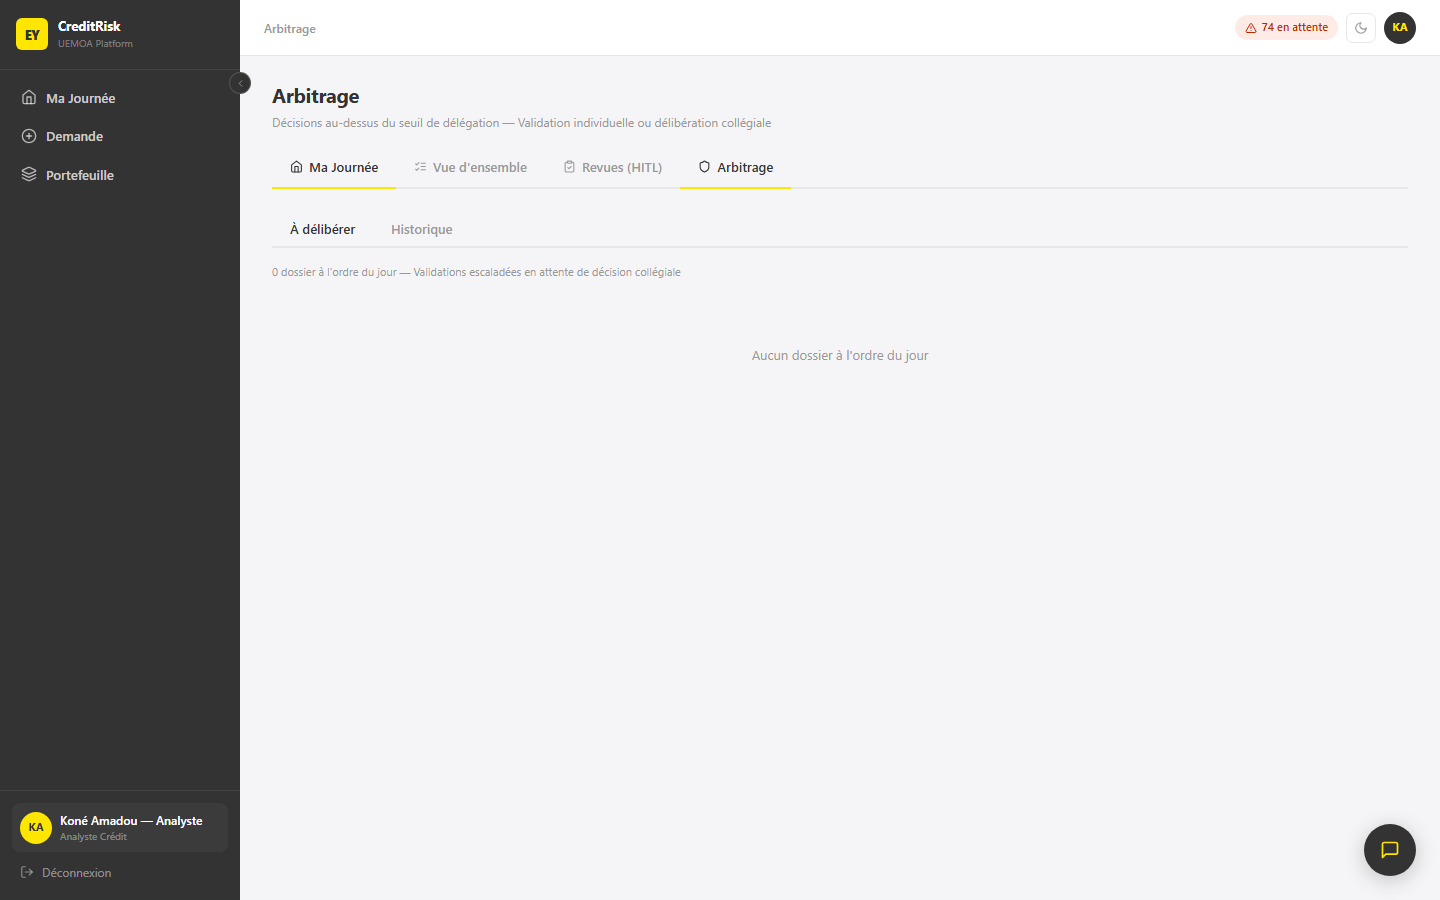
\includegraphics[width=0.85\textwidth]{figures/capture_delegation_arbitrage.png}
\caption{Écran d'arbitrage — décisions au-dessus du seuil de délégation, intégration réelle du service de gouvernance des engagements}
\label{fig:capture-delegation}
\end{figure}

La figure~\ref{fig:capture-delegation} illustre cette intégration : l'écran d'arbitrage, distinct de la file de revues manuelles présentée en section~4.5, n'affiche que les dossiers dont l'exposition dépasse le seuil de délégation de l'analyste connecté, et distingue explicitement la validation individuelle de la délibération collégiale.

\subsection{Réalisation du parcours Portfolio Analytics}

Le traitement batch du portefeuille, détaillé par le diagramme de séquence du chapitre 5, est réalisé par un orchestrateur unique qui enchaîne huit étapes déjà construites indépendamment, sans règle métier qui lui serait propre, de la construction de la population scorée jusqu'au calcul des signaux d'alerte précoce, avant une écriture finale dans l'ensemble des tables concernées au sein d'une unique transaction : toute exception survenant à n'importe quelle étape de cette écriture entraîne l'annulation complète de la transaction, de sorte qu'aucune table ne conserve un run partiellement enregistré. Les différents routeurs exposent les résultats de ce traitement batch pour le suivi général du portefeuille, les projections et les scénarios de stress, ainsi que l'analyse de la rentabilité. Ces traitements mobilisent les modèles entraînés destinés au suivi du portefeuille, présentés au chapitre 3, ainsi que les moteurs complémentaires présentés en section~4.4. Les modèles de probabilité de défaut utilisés dans ce parcours sont distincts de celui mobilisé lors de l'Origination.

\begin{figure}[H]
\centering
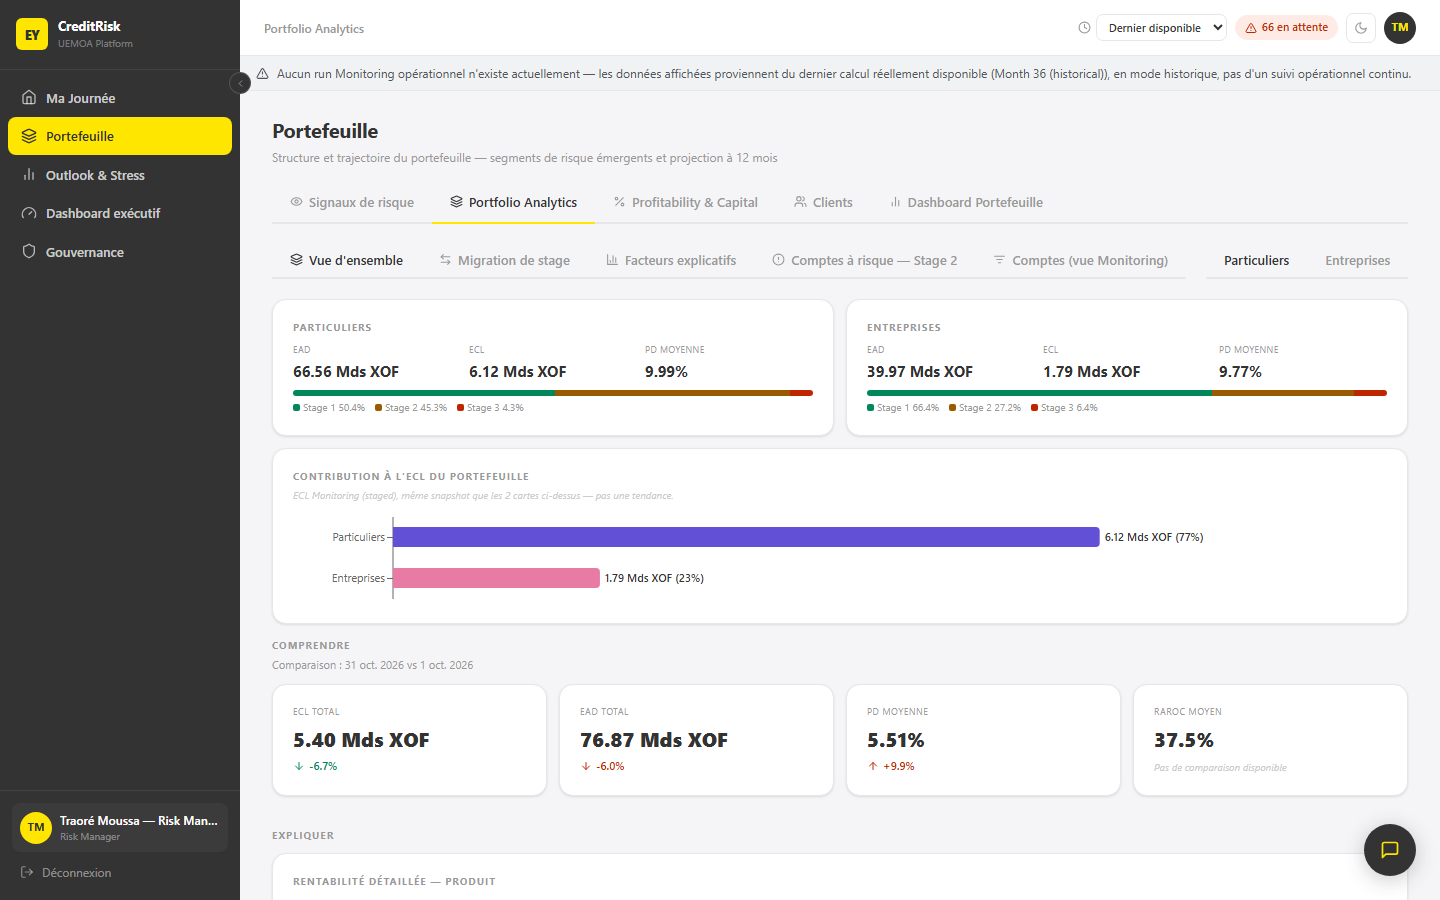
\includegraphics[width=0.85\textwidth]{figures/capture_portfolio_analytics.png}
\caption{Portfolio Analytics — résultats du traitement batch exposés par segment (Particuliers/Entreprises) et par Stage}
\label{fig:capture-portfolio-analytics}
\end{figure}

La figure~\ref{fig:capture-portfolio-analytics} donne à voir ce que recouvre concrètement « le suivi général du portefeuille » : l'exposition, l'ECL et la PD moyenne calculés par le batch, restitués par segment et par Stage, avec un bandeau de provenance qui rappelle explicitement que ces chiffres proviennent du dernier calcul réellement disponible plutôt que d'un suivi opérationnel continu, cohérent avec l'état réel du Monitoring déjà décrit au chapitre 4.

\subsection{Authentification et contrôle d'accès}

L'accès à la plateforme repose sur une authentification par jetons. La connexion d'un utilisateur produit un jeton d'accès de courte durée et un jeton de rafraîchissement, ce dernier conservé en base sous forme hachée plutôt qu'en clair. Le renouvellement d'un jeton d'accès fait tourner ce jeton de rafraîchissement : l'ancien est explicitement révoqué à chaque renouvellement, et la déconnexion révoque également le jeton en cours, de sorte qu'un jeton compromis ne reste pas valide indéfiniment.

Le contrôle d'accès par rôle, présenté au chapitre 2 pour les six rôles réels de la plateforme, chargé de clientèle, analyste crédit, Risk Manager, Direction, Conformité et Audit, Administrateur, n'est pas appliqué au seul niveau de l'interface : il est vérifié côté backend, par un mécanisme d'injection de dépendances propre à chaque point d'entrée de l'API. Ce mécanisme est effectivement mobilisé sur 91 points d'entrée répartis dans l'ensemble des routeurs de la plateforme, qu'il s'agisse de restreindre un endpoint à un rôle unique ou à un ensemble de rôles autorisés. Cette vérification s'exécute au niveau du point d'entrée de l'API lui-même, avant tout traitement métier : une tentative d'accès par un rôle non autorisé est donc rejetée indépendamment de l'interface cliente qui a émis la requête, qu'il s'agisse de l'application web présentée au chapitre 5 ou d'un appel direct à l'API.

\subsection{Traçabilité et gouvernance}

La traçabilité des traitements et des décisions, présentée au chapitre 2, repose sur un journal d'audit chaîné par hachage SHA-256, auquel s'ajoutent plusieurs tables de gouvernance. Les exécutions de la plateforme alimentent notamment les runs de pipeline, qu'ils soient d'entraînement, d'Origination en ligne ou de suivi de portefeuille, de même que les validations humaines requises par la délégation et les tickets de revue manuelle. À ces éléments produits par l'exécution s'ajoute la table des barèmes de délégation, qui relève à l'inverse de la configuration administrative plutôt que d'un événement d'exécution : elle conserve les seuils fixés pour encadrer les décisions, et non une trace de traitement. Cette gouvernance n'est donc pas qu'un mécanisme conçu, mais un ensemble de données réellement produites par les exécutions du projet, parmi lesquelles les runs déjà cités aux chapitres 4 et 5 pour illustrer le stress testing et le suivi de portefeuille.

\begin{figure}[H]
\centering
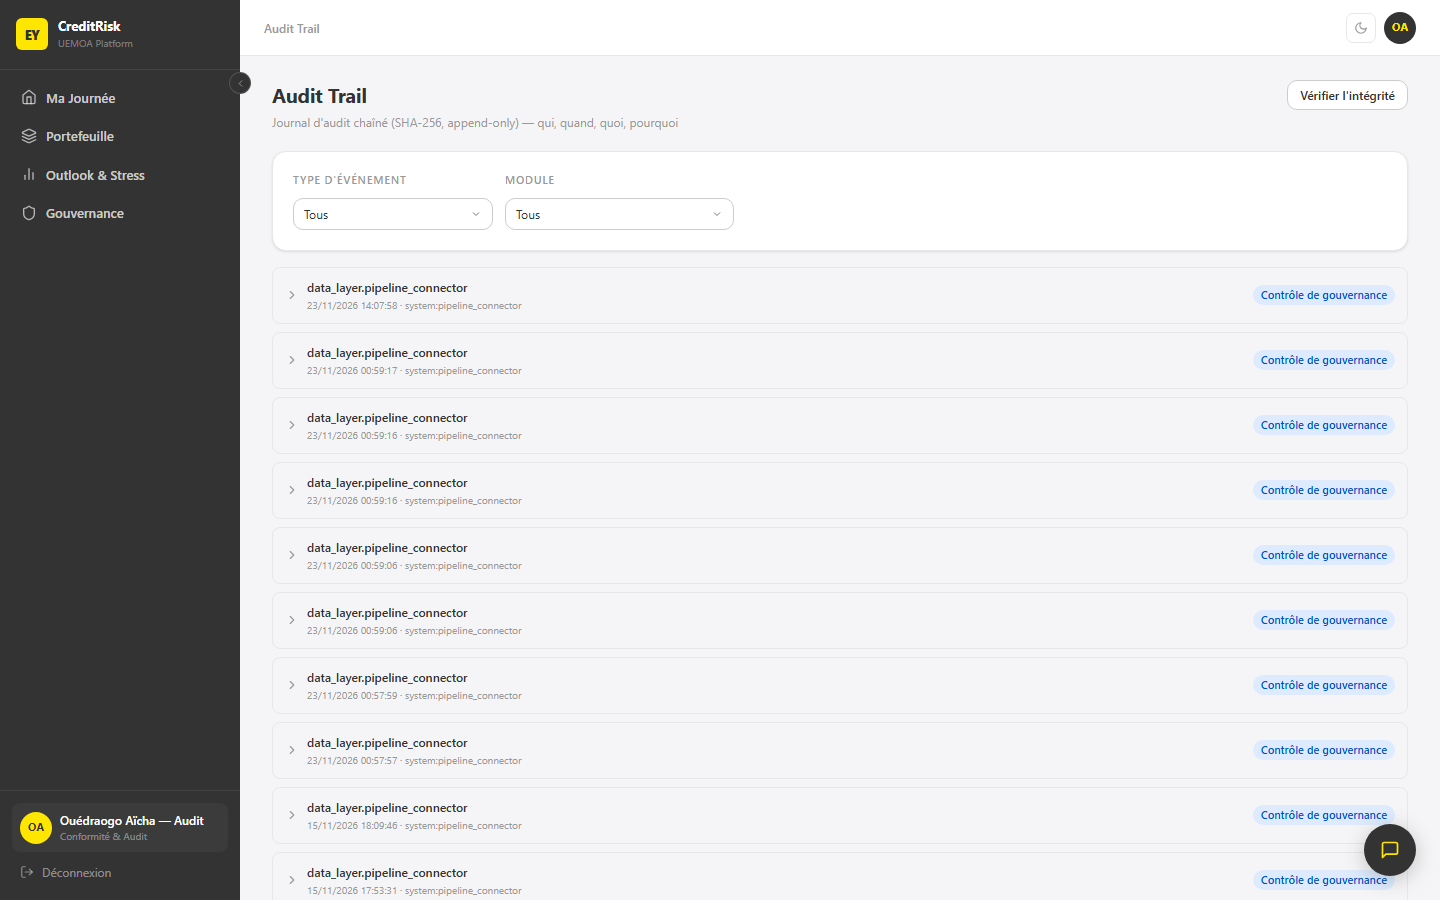
\includegraphics[width=0.85\textwidth]{figures/capture_audit_trail.png}
\caption{Journal d'audit chaîné — qui, quand, quoi, pourquoi, avec vérification d'intégrité}
\label{fig:capture-audit-trail}
\end{figure}

La figure~\ref{fig:capture-audit-trail} montre cette table telle qu'alimentée par l'exécution réelle de la plateforme, avec un bouton de vérification d'intégrité qui permet de contrôler, à tout instant, que la chaîne de hachage n'a pas été rompue.

Le barème de délégation mentionné au chapitre 4 comporte quatre paliers réels, administrés par un rôle Administrateur plutôt que codés en dur : pour le segment Particuliers, une décision reste automatique (AUTO) jusqu'à 5~millions de XOF d'exposition, requiert une validation individuelle (VALIDATION) jusqu'à 20~millions, et passe en comité de crédit (COMITE) au-delà ; pour le segment Entreprises, ces mêmes paliers s'échelonnent à 50~millions, 500~millions puis 2~milliards de XOF, un quatrième palier, le comité exécutif (COMITE\_EXECUTIF), s'appliquant au-delà de ce dernier montant. Ces plafonds sont des paramètres de politique de crédit propres au projet, et non une transposition de seuils réglementaires.

Le suivi du portefeuille mobilise par ailleurs deux autres familles de seuils, distinctes de la politique de décision. Quatre règles réelles déclenchent l'ouverture d'une revue de risque sur un compte déjà en portefeuille : le passage du Stage 1 au Stage 2 depuis l'origination, une hausse de la probabilité de défaut supérieure à 3~points depuis l'origination, un incident de paiement observé sur le dernier mois pour les Particuliers, et au moins deux dégradations de la notation depuis l'origination pour les Entreprises. La stabilité des modèles déployés est par ailleurs surveillée par un indice de stabilité de population (PSI). La plateforme retient les seuils conventionnels suivants pour l'interpréter : un indice inférieur à 0,10 signale une population stable, entre 0,10 et 0,25 une dérive modérée, et au-delà de 0,25 une dérive significative. Un contrôle de qualité des données, enfin, s'exécute en amont de chaque traitement batch, avec un seuil d'avertissement à 50~\% de valeurs manquantes sur une colonne, et un blocage strict en cas de doublons sur la clé naturelle d'une table ou de valeurs nulles sur une colonne clé.

\section{Réalisation de l'assistant intelligent}

\subsection{Intégration de l'assistant dans la plateforme}

Côté frontend, l'assistant n'est pas une page que l'utilisateur ouvrirait séparément : il est monté une seule fois, au niveau du conteneur applicatif (\texttt{AssistantProvider}, englobant \texttt{Layout} dans l'arborescence de composants), au-dessus du point où React Router substitue le contenu des pages. Le composant et son fournisseur restent ainsi montés lors de la navigation entre les écrans présentés en section~6.4 ; le changement de route ne provoque pas leur réinitialisation. Ce fournisseur expose un contexte global à deux niveaux : un contexte d'affichage léger, présenté dans le volet de l'assistant, et un contexte métier, transmis au backend pour contextualiser les requêtes, que chaque page met à jour à son entrée (page courante, type et identifiant de l'entité affichée le cas échéant). Le composant \texttt{FloatingAssistant}, superposé à toutes les pages via un bouton flottant, lit ce contexte pour adapter ses suggestions de questions au rôle de l'utilisateur connecté et à la page courante, et transmet l'identifiant d'entité de la page, lorsqu'il existe, à chaque question posée.

Cette architecture a une conséquence directe sur la résolution d'identité présentée au chapitre 5 : la contextualisation d'une question portant sur une entité affichée ne repose pas sur une résolution de référence à partir de l'historique conversationnel, mais sur l'identifiant de l'entité transmis par la page courante. Une question posée depuis la fiche d'un client porte donc implicitement sur ce client, sans que l'utilisateur ait besoin de le repréciser, tandis qu'une question posée depuis une page sans entité associée, par exemple le tableau de bord du portefeuille, ne porte sur aucun compte en particulier.

\subsection{Orchestration et traitement des requêtes}

Côté backend, un point d'entrée unique, \texttt{POST /api/assistant/ask}, reçoit la question ainsi que le contexte de page transmis par le frontend, puis délègue le traitement à \texttt{AIRiskAssistant.ask()}. Le déroulement complet de cette méthode, du contrôle des droits d'accès jusqu'à la double traçabilité, est représenté par le diagramme de séquence de la figure~\ref{fig:sequence-assistant} (section~5.5) ; cette sous-section présente les choix d'implémentation qui sous-tendent ce flux, sans en reprendre le détail pas à pas.

Le routeur met en œuvre les deux niveaux de classification présentés au chapitre 5 au moyen de mécanismes distincts : une détection par expressions régulières sur des mots-clés associés à chaque catégorie, dont le résultat est retenu dès que le seuil de confiance fixé à 0,70 est atteint, puis, seulement dans le cas contraire, un calcul de similarité cosinus entre l'embedding de la question et des exemples de référence par catégorie. Une question courte, de six mots ou moins, bénéficie en outre d'un mécanisme de contextualisation conversationnelle propre à ce routeur : lorsque la classification demeure incertaine, la catégorie de l'échange précédent est réutilisée plutôt que reclassée à vide. Ce mécanisme répond à une particularité du dialogue en langage naturel, absente des deux autres parcours de la plateforme : une question de relance, telle que « et pour les entreprises ? », ne porte souvent pas assez d'information pour être interprétée indépendamment du tour précédent.

La catégorie retenue est ensuite convertie en \textit{Scope} par une fonction dédiée. En l'absence de correspondance, celle-ci lève une exception plutôt que d'attribuer un périmètre par défaut. Cette vérification rend explicite toute catégorie non prise en charge et évite qu'elle soit traitée dans un périmètre inapproprié.

L'implémentation mutualise également une partie de ce traitement pour une seconde fonctionnalité, la génération d'un brief structuré de dossier client : contrairement à \texttt{ask()}, qui détermine la catégorie à partir de la question, \texttt{generate\_brief()} fixe directement la catégorie à CASE. Les deux méthodes s'appuient ensuite sur la même fonction interne, \texttt{\_answer\_from\_route()}, qui centralise le contrôle des droits, la validation des réponses, l'évaluation automatique et l'écriture en mémoire et dans les journaux d'audit, sans dupliquer ces mécanismes entre les deux usages ; seul l'historique conversationnel transmis au prompt diffère entre les deux, \texttt{generate\_brief()} ne le réutilisant pas, un brief de dossier étant par construction indépendant des échanges précédents.

\subsection{Recherche documentaire et système RAG}

Le moteur de recherche documentaire, déjà présenté au chapitre 5 pour son principe hybride FAISS/BM25, repose sur une boucle itérative de récupération et de vérification, pas une unique passe de recherche. À chaque itération, FAISS et BM25 sont interrogés indépendamment pour produire chacun une cinquantaine de passages candidats, dont l'union, plutôt qu'une fusion pondérée des deux scores, est ensuite reclassée par similarité cosinus entre l'embedding de la requête et celui de chaque passage candidat pour ne retenir que les \texttt{top\_k} passages finalement transmis au prompt. Si la réponse générée contient la mention explicite d'information non disponible, ou si son score de couverture sémantique, tel que nommé dans le code, reste sous un seuil fixé, le nombre de passages recherchés est doublé et une nouvelle itération est lancée, dans la limite de deux itérations de recherche au total par défaut, c'est-à-dire la recherche initiale suivie d'au plus une relance, ce seuil comme le nombre d'itérations maximal restant paramétrables par variable d'environnement. Ce score mesure une similarité cosinus entre le contexte retourné et la réponse produite. Il s'agit d'un indicateur de proximité sémantique, et non d'une vérification factuelle garantissant que chaque élément de la réponse est effectivement justifié par les documents retrouvés. Cette base documentaire étant majoritairement rédigée en anglais, la requête de recherche, mais non la question posée à l'utilisateur, est enrichie de termes anglais équivalents lorsqu'elle contient une expression courante du vocabulaire IFRS 9 en français, afin d'améliorer le rappel sans altérer la question reformulée dans la réponse.

Le contexte documentaire retrouvé, de même que l'historique conversationnel et le contexte de page transmis par le frontend, sont délimités explicitement dans le prompt avant d'y être insérés, jamais traités comme une instruction système, selon deux catégories distinctes définies dans le code : le contexte documentaire, qui ne provient pas du client mais d'une base indexée, et l'historique conversationnel ainsi que le contexte de page, effectivement fournis par le client à chaque requête. Les sources restituées à l'utilisateur, au format « [document - page] », sont extraites par reconnaissance de motif directement depuis le contexte documentaire retrouvé, et non depuis le texte de la réponse générée par le modèle : l'extraction porte sur ce qui a effectivement été récupéré par la recherche hybride, pas sur ce que le modèle a choisi de citer, ce qui limite l'affichage de références absentes du contexte effectivement récupéré, sans garantir pour autant que chaque passage récupéré ait été utilisé dans la réponse elle-même.

\subsection{Génération des réponses et mécanismes de repli}

La génération du texte de réponse repose sur une interface commune, implémentée par deux fournisseurs de génération externes et un fournisseur déterministe de dernier recours, plutôt que sur un modèle unique figé dans le code. Au démarrage de l'assistant, une fonction dédiée retient le premier fournisseur effectivement disponible parmi les trois, dans un ordre fixe : Groq, s'il expose une clé d'API valide et parvient à initialiser son client ; Anthropic sinon, selon le même principe ; le fournisseur déterministe en dernier recours, qui ne dépend d'aucun service externe et reste donc toujours disponible. Cette disponibilité est vérifiée une seule fois, à la construction de l'assistant, et non à chaque question : un fournisseur qui deviendrait indisponible en cours d'exécution, après ce choix initial, ne déclenche pas de bascule automatique vers le suivant.

Le fournisseur de dernier recours ne doit pas être confondu avec un troisième modèle génératif : il ne produit aucun texte original, mais retourne l'une de quelques réponses préécrites, sélectionnée par une simple détection de mots-clés dans la question (Stage 2, ECL, RAROC, motif de rejet). Son rôle n'est pas de répondre correctement à une question arbitraire, mais de fournir une réponse de secours lorsqu'aucun fournisseur de génération externe n'est disponible à l'initialisation, notamment lors d'un développement local sans clé d'API. Cette distinction a une conséquence directe sur l'interprétation d'une réponse de l'assistant au moment des tests ou d'une démonstration : les réponses de ce fournisseur de dernier recours sont fixes pour un même mot-clé détecté, quelle que soit la formulation exacte de la question ou le fil de la conversation, un indice observable que l'assistant fonctionne en mode de repli plutôt qu'avec un fournisseur de génération réel.

\subsection{Sécurité et traçabilité}

Le filtrage RBAC déjà présenté au chapitre 5 est implémenté selon un principe de refus par défaut (\textit{fail-closed}), plutôt que sous la forme d'une liste de restrictions ajoutées au cas par cas : un rôle absent de la table des périmètres autorisés ne se voit attribuer aucune catégorie de donnée sensible. Cette approche évite notamment qu'un périmètre vide soit interprété comme une autorisation illimitée à la suite d'une erreur de configuration. Chaque résultat de requête est filtré récursivement, champ par champ, les catégories étant déterminées à partir de conventions de nommage déjà utilisées dans les moteurs spécialisés (un champ contenant \texttt{shap} ou \texttt{raroc}, par exemple, relève respectivement de l'interprétabilité ou de la rentabilité). Un conteneur dont tous les champs ont été supprimés après filtrage est lui-même retiré du résultat, plutôt que conservé sous la forme d'un objet vide, afin de ne pas exposer indirectement la structure de données non autorisées.

Une fois la réponse assemblée, une seconde couche, distincte du filtrage RBAC, vérifie sa cohérence avant qu'elle n'atteigne l'utilisateur. Cette couche de validation effectue quatre contrôles successifs, chacun pouvant à lui seul entraîner le rejet de la réponse entière : l'ancrage, qui rejette une réponse lorsque des faits vérifiables sont disponibles mais qu'aucun n'est cité ; la validité des références, qui doivent toutes correspondre à un fait effectivement fourni au modèle ; la provenance, chaque fait cité étant revérifié à partir de son artefact source exact ; et la cohérence avec l'écran, pour les faits disposant d'une méthode de vérification dédiée, la valeur citée étant comparée à celle réellement affichée par l'interface. Cette couche ne garantit pas l'exactitude de toute réponse produite. Elle réduit le risque qu'un fait explicitement vérifiable soit présenté alors que sa validité n'est plus confirmée par sa source. Elle ne garantit toutefois pas l'exactitude de l'ensemble du texte formulé librement par le modèle autour de ces faits.

Une évaluation automatique complémentaire est également réalisée, sans se substituer à cette validation : elle combine des métriques de similarité entre les embeddings du contexte et de la réponse avec un jugement produit par un second appel au modèle de langage, selon des critères de correction, de fidélité, d'absence d'hallucination et de pertinence métier. Cette évaluation repose donc elle-même sur un modèle de langage chargé de juger la réponse d'un autre modèle. Son résultat est journalisé à titre d'indicateur de suivi et n'intervient pas dans la décision de rejeter ou non la réponse, déjà prise par la couche de validation précédente.

Enfin, chaque interaction fait l'objet de deux enregistrements indépendants : une entrée dans le journal dédié à l'assistant, propre à ce sous-système, et une entrée dans le journal d'audit central de la plateforme, présenté au chapitre 2. La seconde écriture est conçue pour être non bloquante : un échec de l'enregistrement dans le journal d'audit central est intercepté et ne doit pas interrompre le traitement de la réponse. Ainsi, une indisponibilité de ce mécanisme de traçabilité ne bloque pas, à elle seule, la restitution d'une réponse déjà produite et validée.

\section{Interface et parcours utilisateurs}

Alors que la section 6.2 démontrait, par quelques captures ciblées, l'intégration technique des modules décrits au chapitre 5, cette section présente l'ensemble des interfaces fonctionnelles réellement accessibles, organisées non par module technique mais par parcours utilisateur. La structure retenue suit l'arborescence de navigation réellement implémentée (\texttt{App.jsx}, \texttt{navigation.js}) plutôt qu'un découpage reconstruit a posteriori : six destinations de premier niveau, accessibles depuis la barre latérale selon le rôle de l'utilisateur connecté, auxquelles s'ajoutent l'écran de connexion et l'assistant conversationnel, ce dernier n'étant pas une destination de navigation mais un composant flottant superposé à l'ensemble de ces écrans. Chaque parcours est présenté sous la forme d'une courte user story, acteur, objectif, interaction et résultat, illustrée par une capture d'écran réelle ; les rôles mentionnés sont strictement ceux effectivement autorisés par le contrôle d'accès présenté en section~6.2.3, aucun acteur ni aucune permission n'étant ici supposés.

\subsection{Accès à la plateforme}

\begin{description}
\item[Acteur] Tout utilisateur détenteur d'un compte, quel que soit son rôle.
\item[Objectif] Accéder à son espace de travail.
\item[Interaction] Saisie de l'identifiant et du mot de passe, puis authentification par jeton présentée en section~6.2.3.
\item[Résultat] Redirection vers l'espace « Ma Journée », dont le contenu dépend du rôle authentifié.
\end{description}

\begin{figure}[H]
\centering
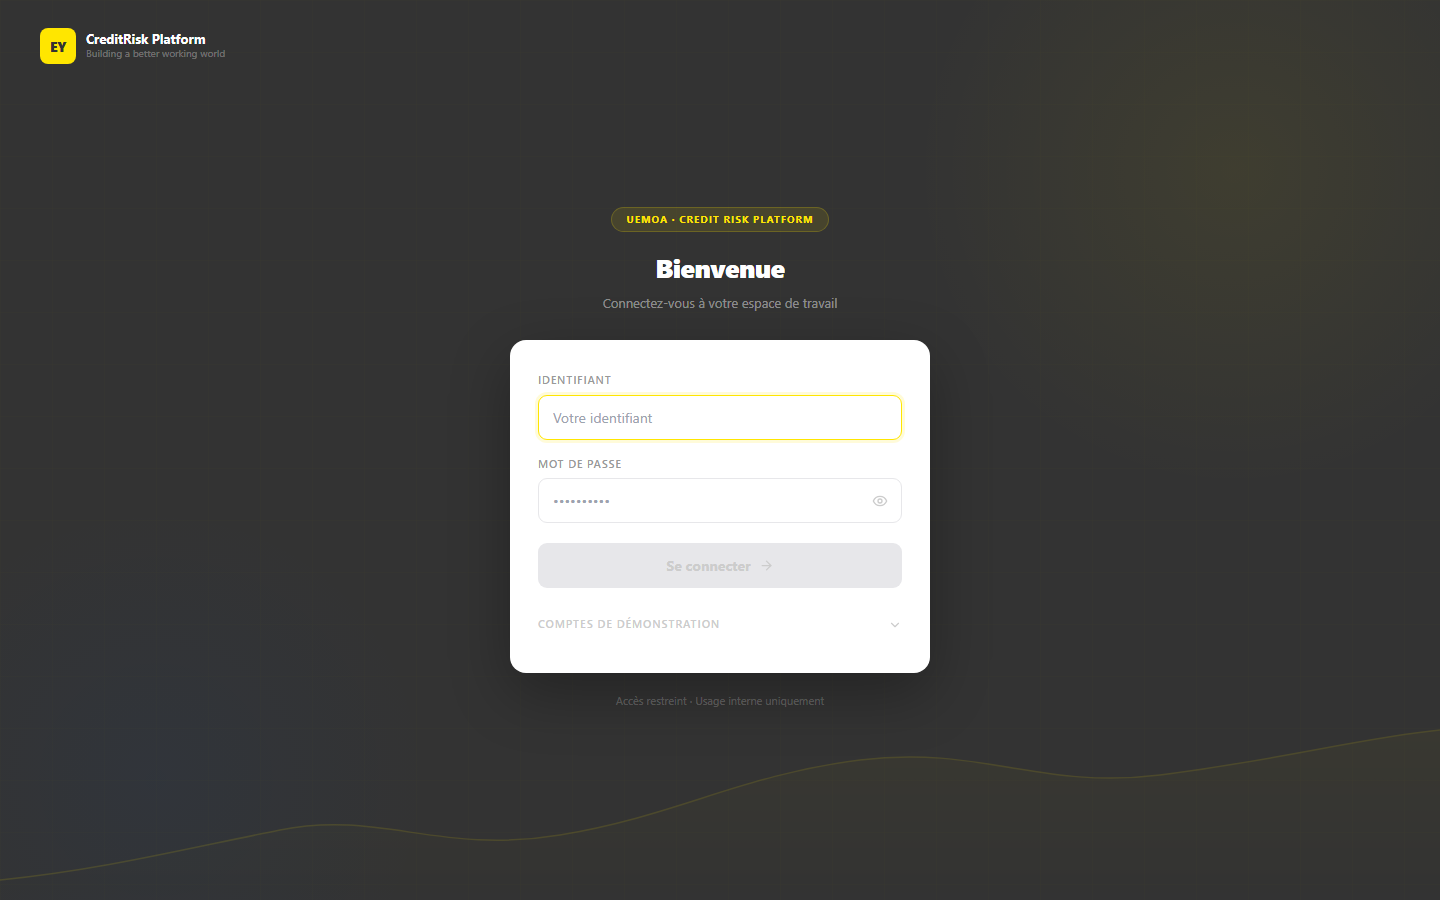
\includegraphics[width=0.6\textwidth]{figures/capture_login.png}
\caption{Écran de connexion}
\label{fig:capture-login}
\end{figure}

\subsection{Ma Journée}

\begin{description}
\item[Acteur] Analyste crédit ou Risk Manager.
\item[Objectif] Suivre les dossiers à traiter dans la journée : revues manuelles en zone grise, et, le cas échéant, dossiers à arbitrer au-delà du seuil de délégation.
\item[Interaction] Consultation de la vue d'ensemble, qui agrège sept sources de travail actionnable, puis ouverture de l'onglet « Revues (HITL) » pour traiter une décision en zone grise nécessitant un arbitrage humain.
\item[Résultat] La liste des revues en attente, filtrable par statut et par segment, permet à l'analyste de sélectionner un dossier et de rendre sa décision.
\end{description}

\begin{figure}[H]
\centering
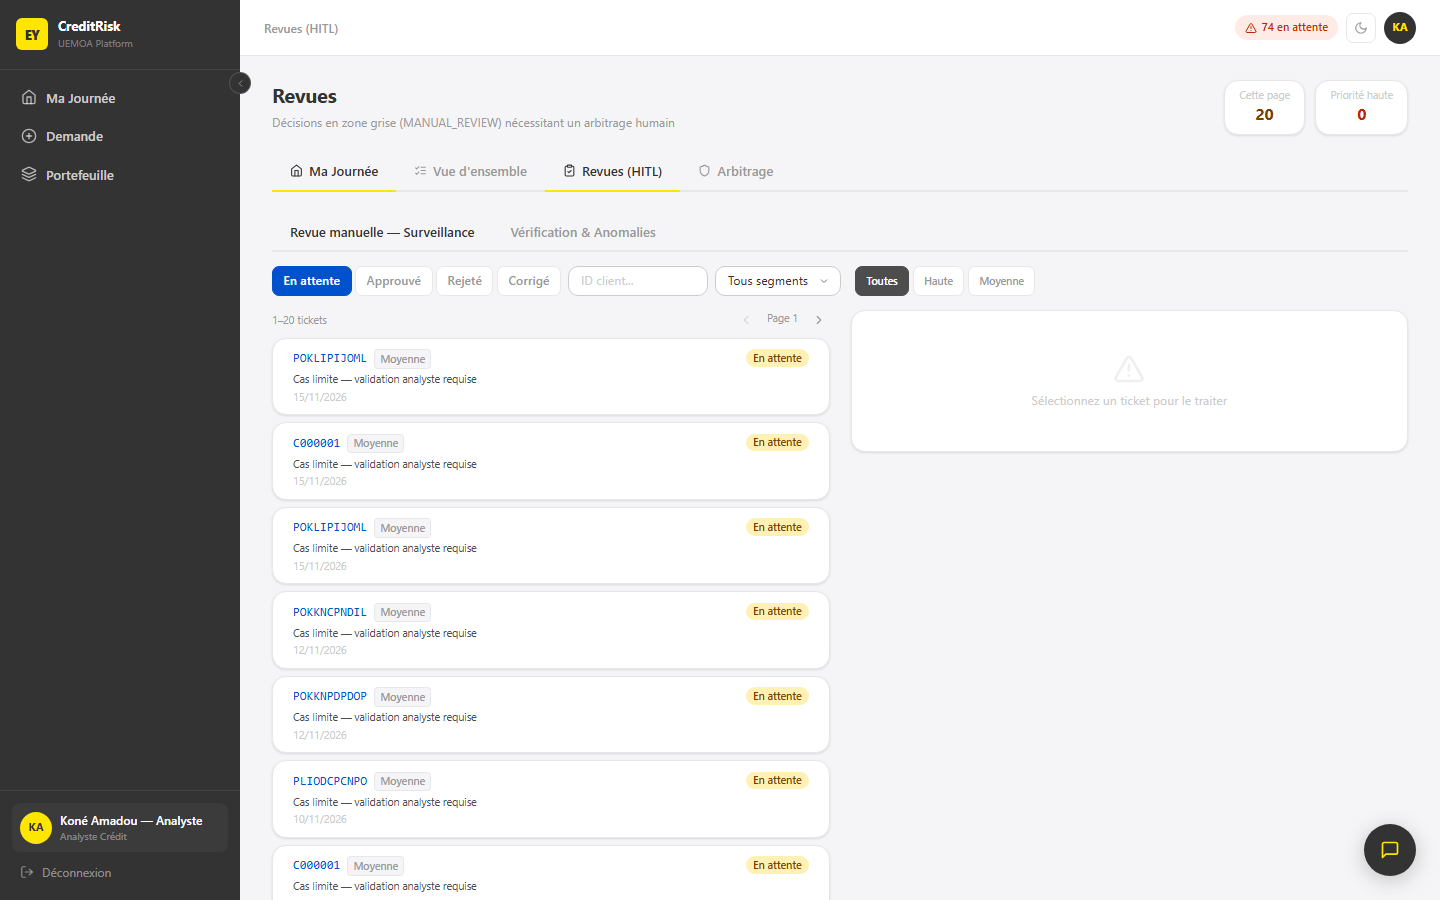
\includegraphics[width=0.85\textwidth]{figures/capture_hitl.png}
\caption{Ma Journée — Revues (HITL), décisions en zone grise nécessitant un arbitrage humain}
\label{fig:capture-hitl}
\end{figure}

\subsection{Demande}

\begin{description}
\item[Acteur] Chargé de clientèle (analyste crédit également habilité).
\item[Objectif] Créer une nouvelle demande de crédit pour un client existant, puis suivre les dossiers déjà engagés.
\item[Interaction] Sélection du client, puis progression dans un parcours en six étapes, demande, situation, risque de la demande, décision, explication et action, avant de retrouver le dossier dans la liste « Dossiers ». Dès la première étape, le chargé de clientèle peut transmettre un document du client, bulletin de salaire, relevé bancaire ou bilan selon le segment ; une extraction réelle, à partir du texte directement extrait du document ou, pour un document scanné sans texte extractible, d'une reconnaissance optique de repli, puis structurée par un modèle de langage, en déduit automatiquement plusieurs champs du formulaire, chacun assorti d'un niveau de confiance, les champs dont la confiance reste sous un seuil de 0,75 étant explicitement signalés et devant être confirmés ou corrigés avant de poursuivre. La dernière étape diffère selon l'issue remappée à l'écran, accord, refus ou à revoir : un accord sous conditions y ouvre un panneau de résolution des conditions, soumis à une permission dédiée, tandis qu'un refus ou un dossier à revoir donne accès, lorsqu'elle est disponible, à l'explication contrefactuelle déjà produite par le moteur, ainsi qu'à un simulateur \textit{What-If} réel permettant d'évaluer l'effet d'un paramètre modifié sur le résultat, sans modifier le dossier initial ni remplacer sa décision enregistrée.
\item[Résultat] Chaque dossier conserve son statut, complet, à revoir ou clôturé, avec son issue, accord, refus ou à revoir, et le montant associé.
\end{description}

\begin{figure}[H]
\centering
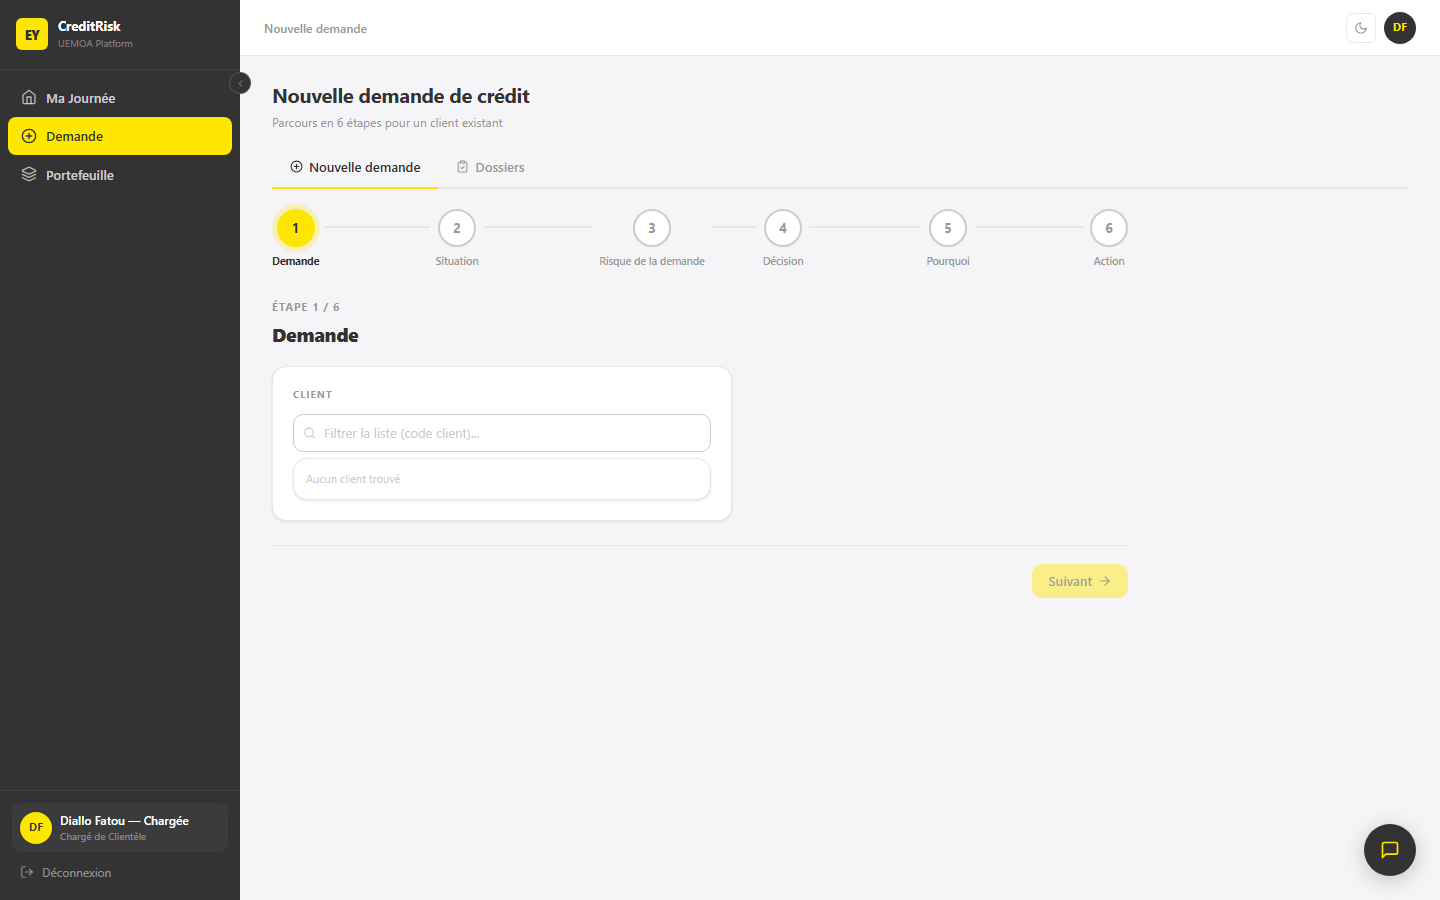
\includegraphics[width=0.85\textwidth]{figures/capture_demande_nouvelle.png}
\caption{Demande — parcours en six étapes de création d'une demande de crédit}
\label{fig:capture-demande-nouvelle}
\end{figure}

\begin{figure}[H]
\centering
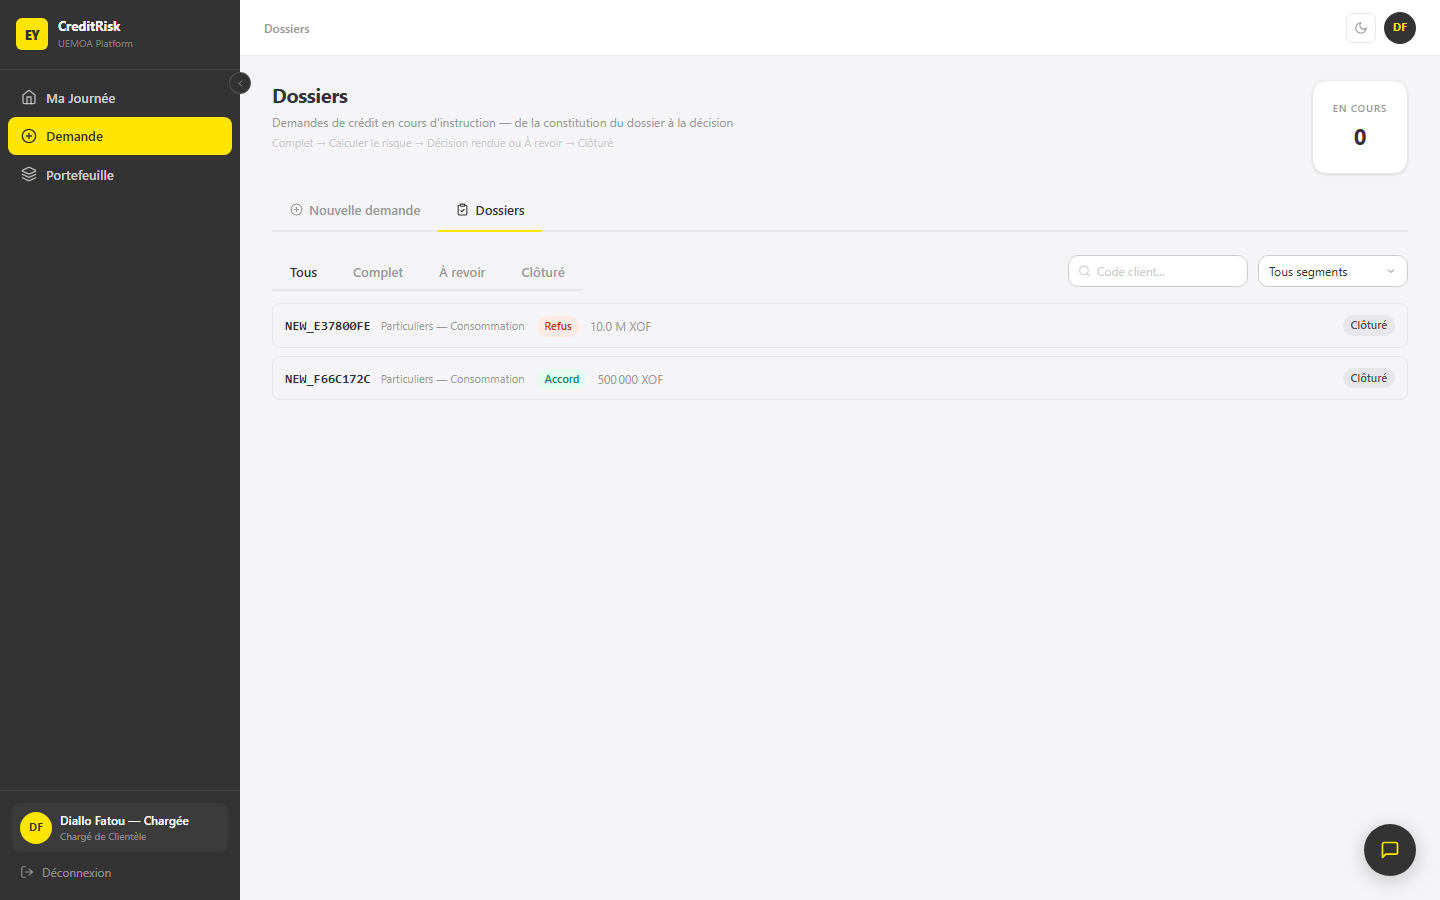
\includegraphics[width=0.85\textwidth]{figures/capture_demande_dossiers.png}
\caption{Demande — suivi des dossiers, de leur instruction à leur décision}
\label{fig:capture-demande-dossiers}
\end{figure}

\subsection{Portefeuille}

\begin{description}
\item[Acteur] Risk Manager, dont le périmètre couvre l'ensemble des cinq onglets de cette destination (l'Exécutif et l'analyste crédit n'y accèdent que partiellement).
\item[Objectif] Explorer la composition et la trajectoire du portefeuille : signaux de risque, analyse détaillée par segment et par Stage, rentabilité et capital, fiche Client 360°.
\item[Interaction] Consultation du tableau de bord Portefeuille, synthèse native du traitement batch présenté en section~6.2.2, puis navigation vers les onglets de détail selon le besoin.
\item[Résultat] Une vue de la composition du portefeuille par segment et par Stage, avec sa tendance par rapport au run précédent, et un bandeau de provenance rappelant explicitement l'origine des données affichées.
\end{description}

\begin{figure}[H]
\centering
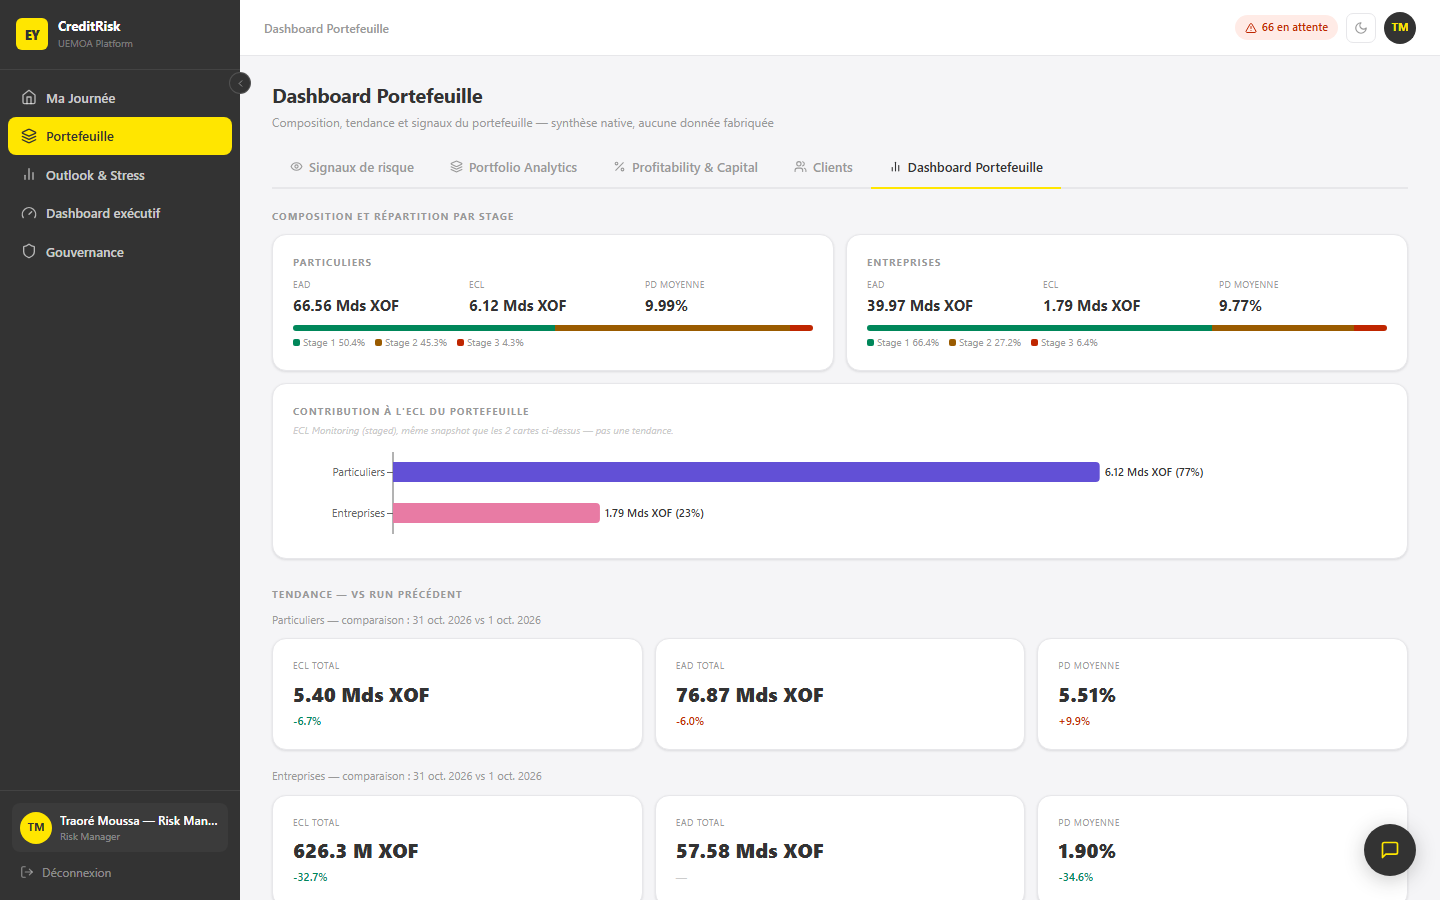
\includegraphics[width=0.85\textwidth]{figures/capture_portfolio_dashboard.png}
\caption{Portefeuille — tableau de bord natif, composition et tendance par rapport au run précédent}
\label{fig:capture-portfolio-dashboard}
\end{figure}

\subsection{Outlook \& Stress}

\begin{description}
\item[Acteur] Risk Manager (Exécutif et Conformité également habilités).
\item[Objectif] Examiner l'évolution projetée du portefeuille et sa résistance à des chocs macroéconomiques hypothétiques, présentées en section~4.4.
\item[Interaction] Consultation de l'onglet Outlook, qui restitue la projection à douze mois glissants par Stage IFRS9 avec sa bande d'incertitude P5/P50/P95, avant de basculer, au besoin, vers les onglets Stress Testing ou Capital \& Policy Simulation.
\item[Résultat] Une trajectoire indicative assortie d'avertissements méthodologiques explicites : la projection n'est pas un engagement chiffré, et la bande d'incertitude statistique ne doit pas être confondue avec l'impact d'un scénario de stress macroéconomique.
\end{description}

\begin{figure}[H]
\centering
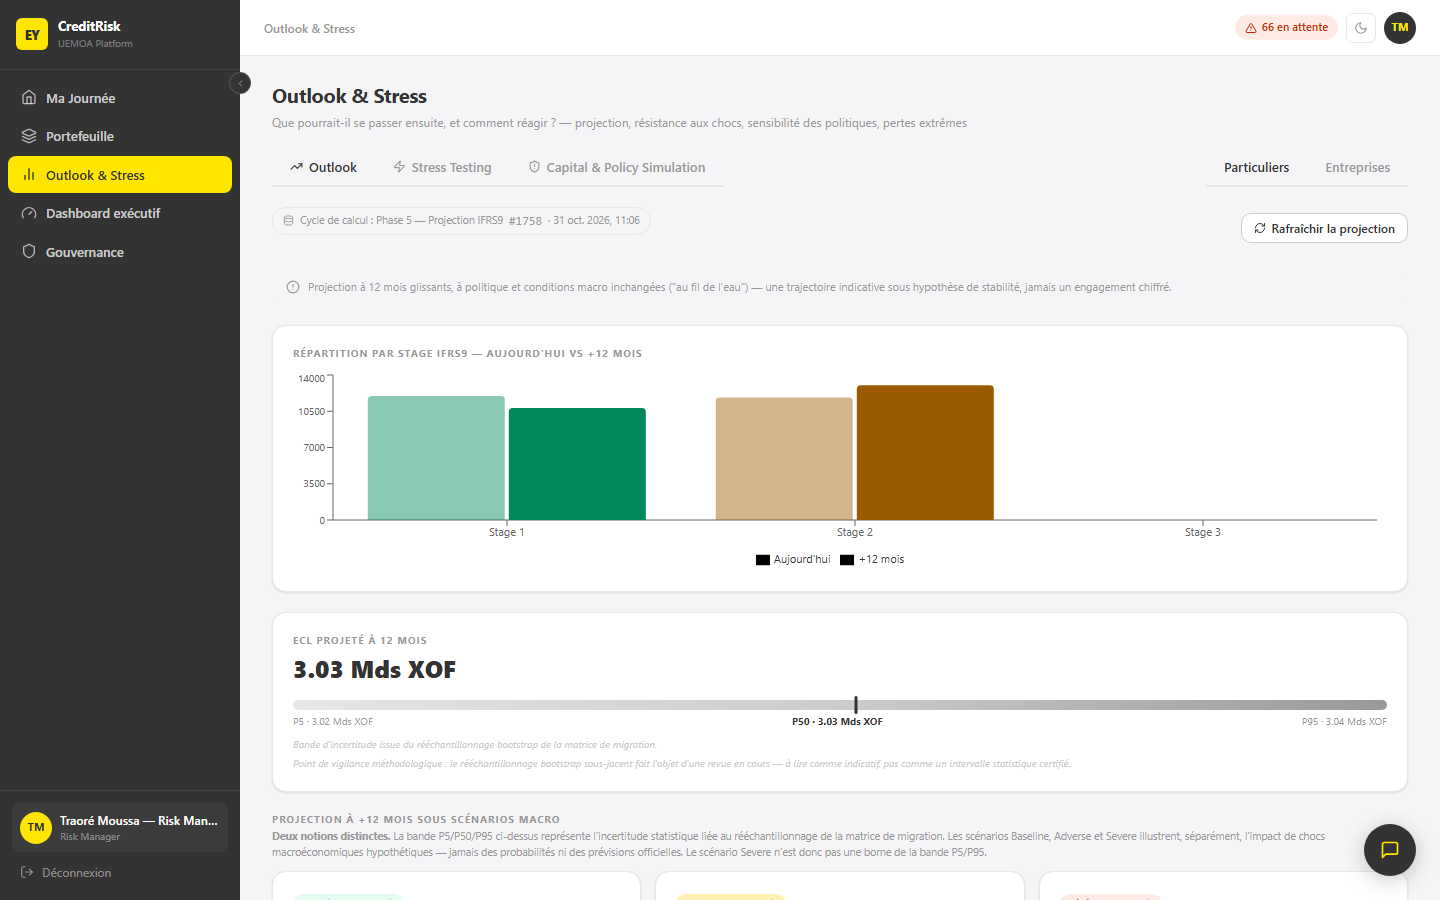
\includegraphics[width=0.85\textwidth]{figures/capture_outlook_stress.png}
\caption{Outlook \& Stress — projection à 12 mois par Stage IFRS9, avec bande d'incertitude et avertissements méthodologiques}
\label{fig:capture-outlook-stress}
\end{figure}

\subsection{Dashboard exécutif}

\begin{description}
\item[Acteur] Direction (Risk Manager également habilité).
\item[Objectif] Disposer d'une synthèse transversale pour le pilotage de l'activité, sans capacité opérationnelle.
\item[Interaction] Consultation du dashboard exécutif, qui agrège en lecture seule les indicateurs déjà présentés dans les autres destinations, exposition, pertes attendues, capital, rentabilité et résultats des stress tests, sans dupliquer leur calcul.
\item[Résultat] Une vue consolidée qui rend explicites, plutôt que de les masquer, les limites méthodologiques déjà rencontrées au chapitre 4 : les deux bases de capital, proxy réglementaire et Monte Carlo, restent présentées séparément et jamais sommées, et le RAROC agrégé au niveau du portefeuille est signalé comme non consolidé faute de convention d'agrégation unique entre les différents pipelines.
\end{description}

\begin{figure}[H]
\centering
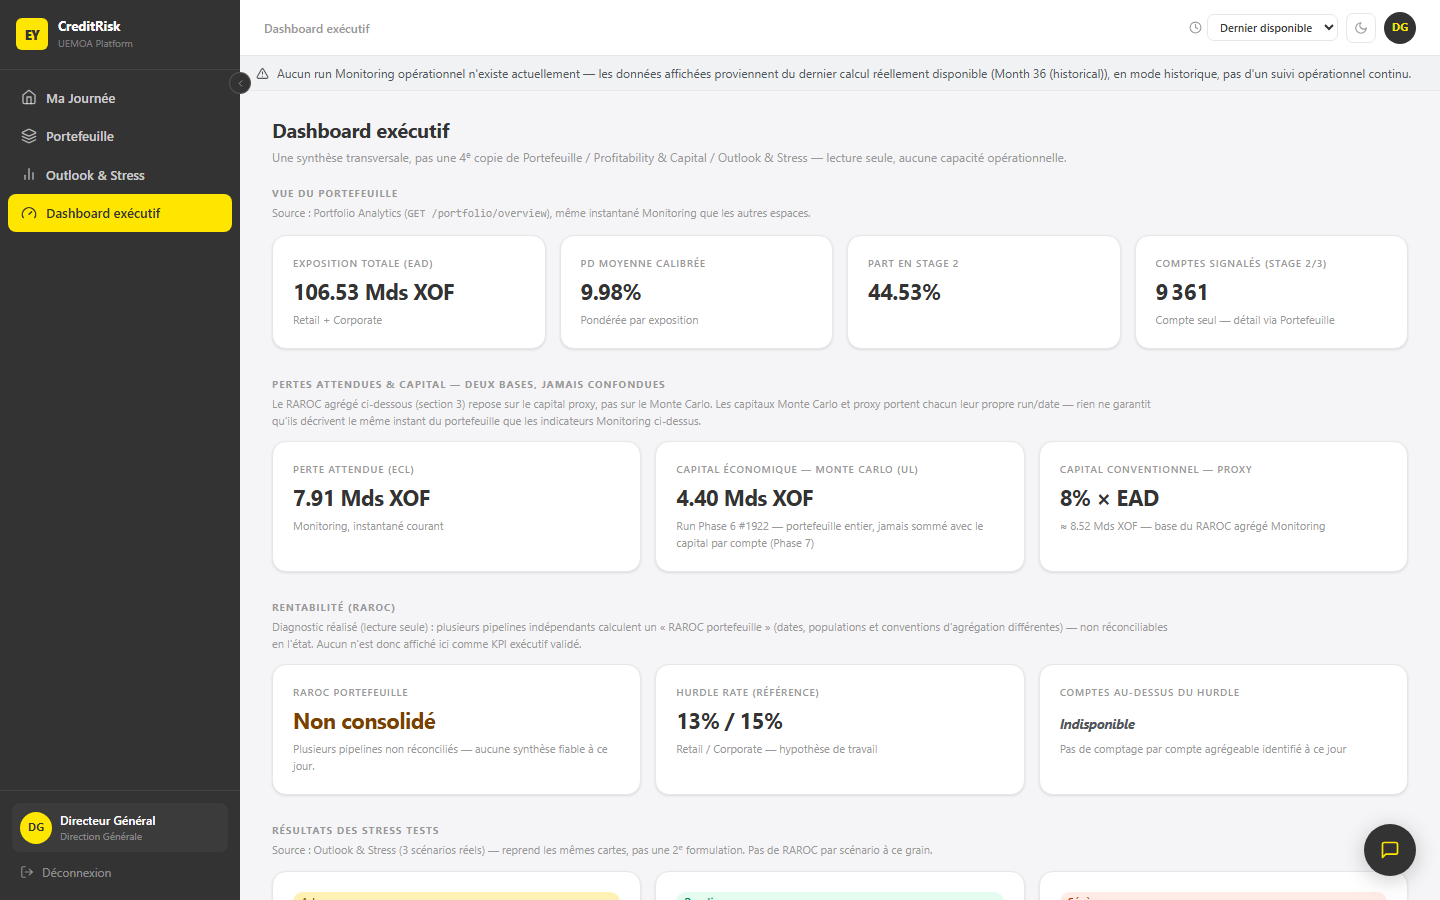
\includegraphics[width=0.85\textwidth]{figures/capture_dashboard_executif.png}
\caption{Dashboard exécutif — synthèse transversale en lecture seule, capital proxy et Monte Carlo jamais confondus}
\label{fig:capture-dashboard-executif}
\end{figure}

\subsection{Gouvernance}

\begin{description}
\item[Acteur] Conformité et Audit pour l'audit trail, la politique de décision, l'inventaire des modèles et les traitements batch ; Administrateur, seul habilité, pour les seuils de délégation et la gestion des utilisateurs et rôles ; Risk Manager pour les Trigger Rules.
\item[Objectif] Consulter, et selon son rôle administrer, les mécanismes de contrôle de la plateforme.
\item[Interaction] Ouverture du hub Gouvernance, dont les sept cartes renvoient chacune vers l'écran réel correspondant avec le même contrôle d'accès que la navigation : une carte à laquelle l'utilisateur connecté n'est pas habilité apparaît grisée, verrouillée et explicitement annotée « Non accessible à votre rôle », plutôt que d'être simplement absente.
\item[Résultat] Pour un compte Conformité et Audit, quatre cartes sur sept sont accessibles, audit trail, politique de décision, modèles, traitements batch, les trois autres restant verrouillées, ce qui illustre concrètement que ce hub ne correspond pas à un acteur unique mais à plusieurs périmètres de rôle distincts. Les cartes Seuils de délégation et Trigger Rules donnent accès aux paramètres déjà présentés en section~6.2.4.
\end{description}

\begin{figure}[H]
\centering
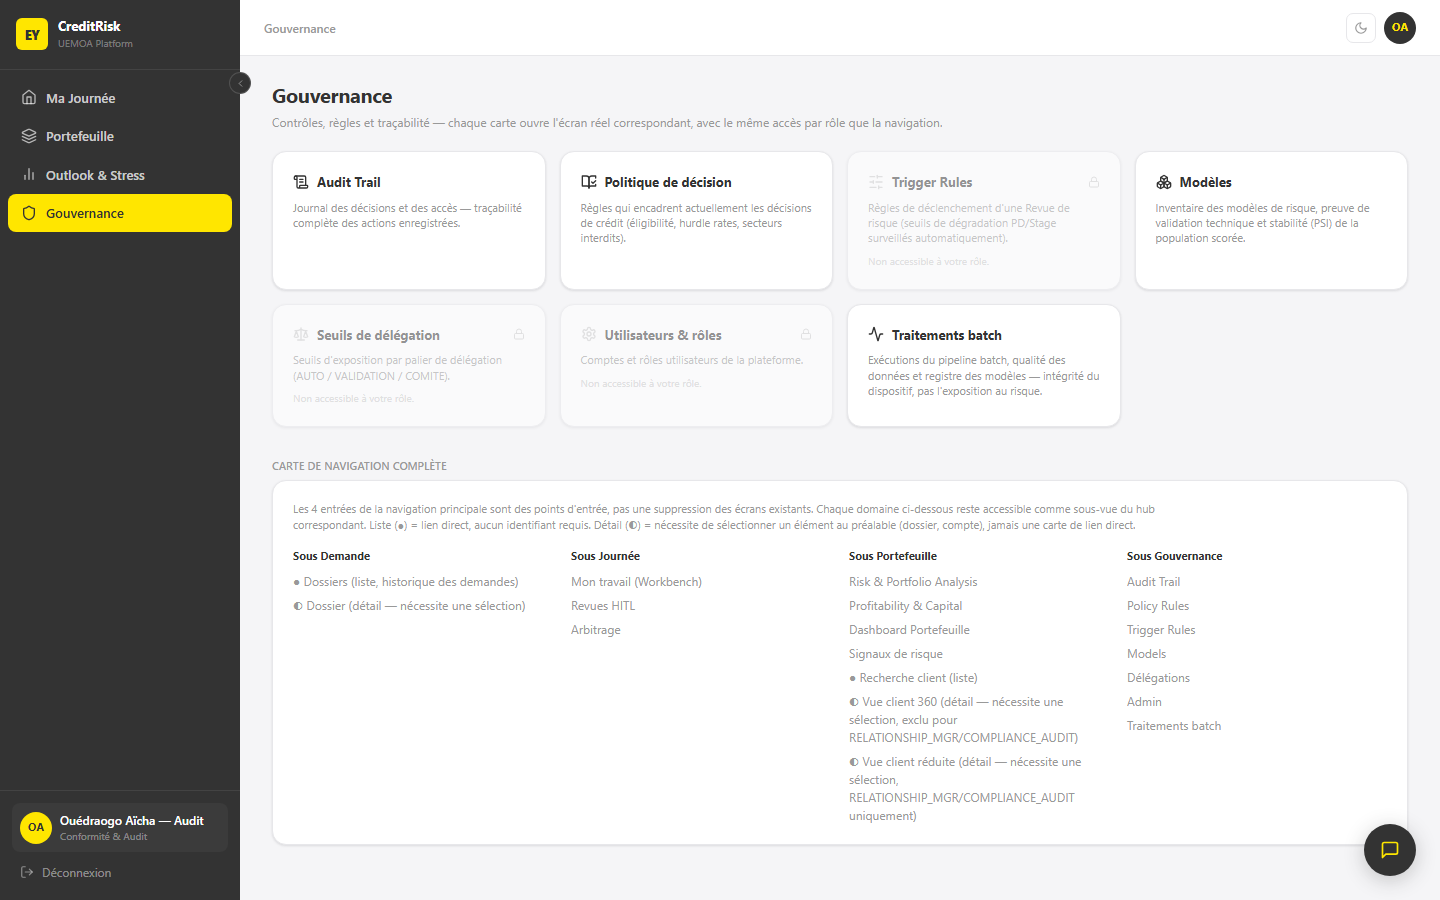
\includegraphics[width=0.85\textwidth]{figures/capture_gouvernance_hub.png}
\caption{Hub Gouvernance — sept cartes, contrôle d'accès visible par carte (vue Conformité et Audit)}
\label{fig:capture-gouvernance-hub}
\end{figure}

\subsection{Assistant transversal}

\begin{description}
\item[Acteur] Tout utilisateur authentifié.
\item[Objectif] Obtenir, depuis n'importe quel écran, une réponse contextualisée sans interrompre son parcours.
\item[Interaction] Ouverture du composant flottant, visible en superposition sur l'ensemble des écrans précédents, puis formulation d'une question en langage naturel.
\item[Résultat] Une réponse contextualisée, qui peut s'appuyer sur la base documentaire réglementaire présentée au chapitre 5 et restituer les références documentaires correspondantes lorsqu'elles sont disponibles, ou sur les moteurs métier du portefeuille et des dossiers clients selon la nature de la question ; lorsque les éléments accessibles ne permettent pas de répondre précisément, l'assistant le signale plutôt que de produire une réponse non étayée.
\end{description}

\begin{figure}[H]
\centering
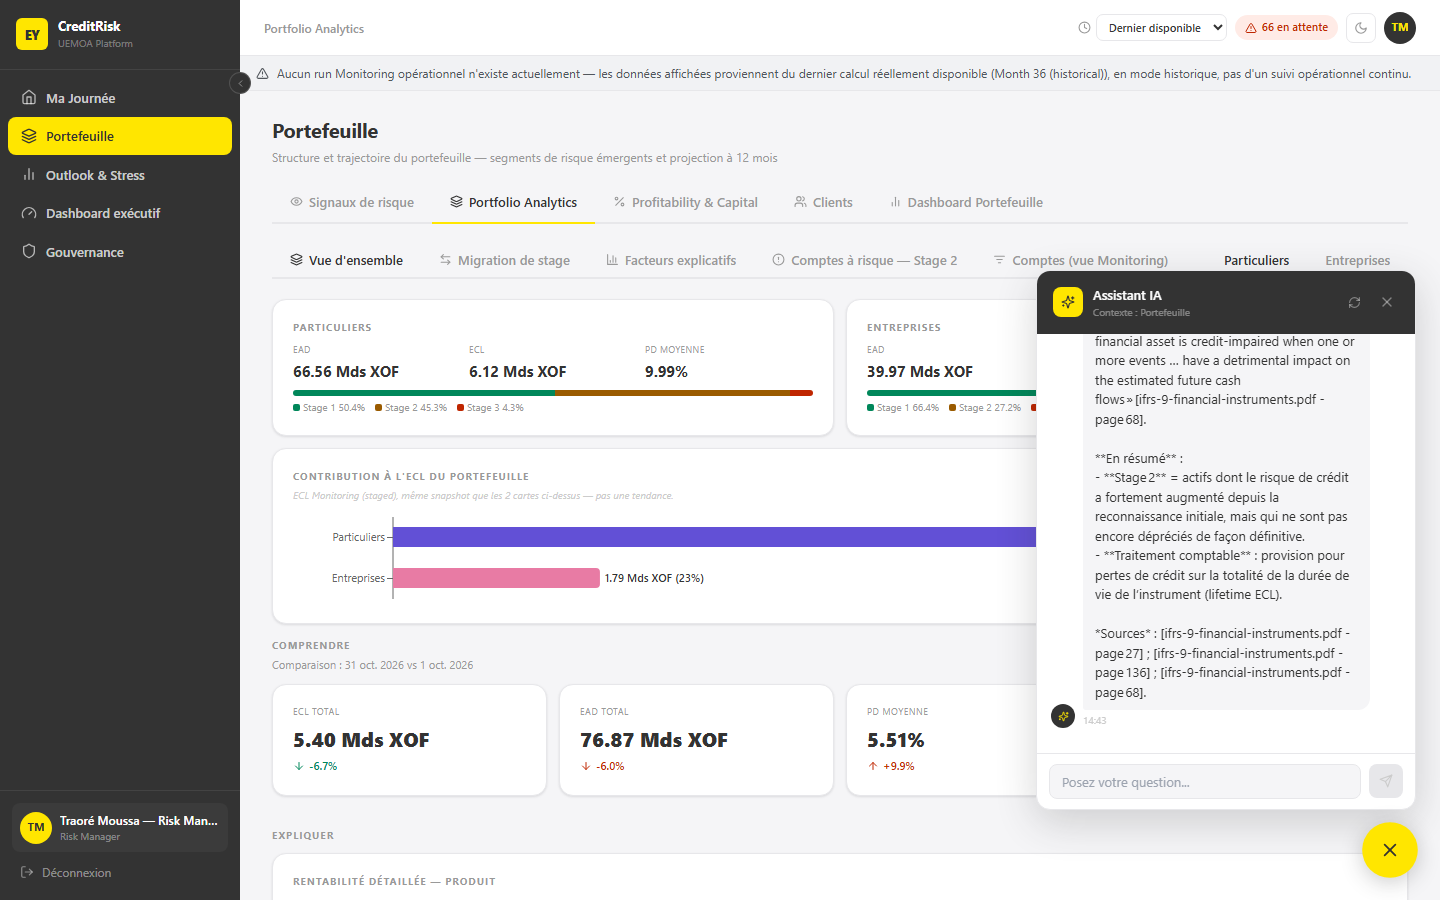
\includegraphics[width=0.85\textwidth]{figures/capture_assistant.png}
\caption{Assistant transversal — réponse appuyée sur la base documentaire réglementaire, avec citation de la source}
\label{fig:capture-assistant}
\end{figure}

\section{Tests et validation}

La stratégie de validation repose sur quatre marqueurs \texttt{pytest} réels, présentés en section~6.1, unitaire, intégration base de données, chaîne de traitement et acceptation, auxquels s'ajoutent, distincts de ce quatrième marqueur, deux scénarios d'acceptation en conditions de navigateur réel, exécutés séparément via Playwright. Les résultats présentés ci-dessous sont ceux d'une exécution réelle de l'ensemble de ces suites, et non des chiffres de référence : chaque échec rencontré a été rejoué isolément, et pour les plus significatifs directement inspecté dans ses artefacts (fichiers de données, journal d'audit), afin d'en caractériser la nature et, lorsque les éléments disponibles le permettent, d'en identifier la cause, plutôt que de les rapporter tels quels depuis un premier passage.

\subsection{Tests unitaires}

La suite unitaire, 351 tests collectés sur des composants isolés sans dépendance système réelle, s'exécute entièrement avec succès : 349 réussis, 2 ignorés, aucun échec.

\subsection{Tests d'intégration base de données}

La suite d'intégration, exécutée contre une instance PostgreSQL réelle, comporte 619 tests marqués, dont 614 réussis, 2 ignorés et 3 échecs, tous dans le même fichier (\texttt{test\_online\_data\_purity.py}). Ces trois échecs partagent une cause commune, confirmée en les rejouant isolément : trois assertions comparent le nombre de décisions en ligne authentiques à une valeur figée, 170, verrouillée au moment de la rédaction du contrat de test correspondant (2026-09-16), alors que la base contient désormais 449 décisions de ce type, un écart qui reflète l'usage réel de la plateforme accumulé depuis cette date plutôt qu'une régression. Le mécanisme d'exclusion lui-même reste par ailleurs démontré correct par ces mêmes échecs : les deux grandeurs comparées à la valeur figée, le décompte brut filtré et la vue \texttt{LIVE}, restent strictement égales entre elles (449 de part et d'autre), ce qui est précisément ce que le test cherche à vérifier au-delà du chiffre lui-même.

\subsection{Tests de chaîne de traitement}

La suite de pipeline, 341 tests marqués, totalise 334 réussis, 1 ignoré et 6 échecs. Cinq de ces six échecs relèvent de la même famille que les échecs d'intégration ci-dessus, une valeur ou un artefact figé devenu obsolète plutôt qu'une régression fonctionnelle : un test attend 60 lignes dans la dimension temporelle du Monitoring et en trouve 179, la couverture temporelle réelle s'étant élargie depuis l'écriture du test ; trois tests lisent un export Parquet des features Particuliers antérieur à l'ajout de certains champs aujourd'hui mobilisés par la plateforme (\texttt{revenu\_mensuel\_xof}, \texttt{stabilite\_profil}), confirmés par ailleurs omniprésents dans le code source actuel, du service de crédit en ligne au moteur d'explication ; un quatrième test, dépendant du même export, échoue en cascade faute de retrouver le premier identifiant client de ce fichier devenu obsolète dans l'état actuel de la plateforme. Le sixième échec est d'une nature différente : la validation d'un document dont le chemin de fichier n'existe pas renvoie \texttt{is\_valid=True} plutôt que \texttt{False}, le pipeline d'extraction ne consignant aucune erreur de validation pour un fichier absent avant le calcul de ce statut.

\subsection{Tests d'acceptation}

Le quatrième marqueur \texttt{pytest}, distinct des scénarios navigateur présentés plus loin, comporte 37 tests répartis sur plusieurs scénarios métier complets (création puis scoring d'un dossier réel, accord sous conditions jusqu'à leur résolution). 27 réussissent, 10 échouent, répartis en deux anomalies réelles et distinctes, toutes deux rejouées et inspectées directement pour en établir la cause.

La première touche neuf tests, répartis sur deux fichiers de scénario dont l'un des paramètres de la demande (profil \emph{Fonctionnaire}, garantie de type caution, ratio de couverture à 1,00) est quasiment identique : dans le premier fichier, un dossier réellement créé et scoré au cours de ce passage présente une exposition, une PD et un hurdle rate persistés à zéro, trois assertions qui en dépendent échouant en conséquence ; dans le second, c'est l'étape initiale du scénario qui échoue directement, sur une erreur Python (\texttt{TypeError}, valeur \texttt{None} inattendue), les cinq étapes suivantes échouant alors en cascade faute de retrouver l'état qu'elles présupposent. Ces deux échecs partagent un profil de demande très proche et pourraient relever d'une même cause, sans que cette campagne de validation permette de l'affirmer avec certitude : l'établir précisément dépasserait le cadre de cette synthèse et relèverait d'une correction à part entière.

La seconde anomalie, isolée, porte sur l'intégrité du journal d'audit chaîné présenté au chapitre 2 : \texttt{verify\_integrity()} détecte une rupture de la chaîne de hachage. L'inspection directe du fichier concerné situe précisément cette rupture : deux entrées \texttt{DATA\_ACCESS} de l'assistant, consécutives, portent un horodatage strictement identique à la microseconde (deux questions quasiment identiques posées le 2026-09-29) et référencent toutes deux le hachage de l'entrée qui les précède, au lieu que la seconde référence le hachage de la première. Il s'agit d'une véritable condition de concurrence sur l'écriture de ce journal en cas d'appels strictement simultanés, antérieure à cette campagne de validation, et non d'une altération a posteriori du journal ni d'un artefact introduit par l'exécution des tests eux-mêmes.

\subsection{Tests d'acceptation en conditions de navigateur}

Les deux scénarios Playwright, séparés du quatrième marqueur \texttt{pytest} ci-dessus, couvrent chacun un parcours bout en bout complet, en conditions de navigateur réel : Origination (client existant jusqu'au Cas Crédit, en passant par la création du dossier et le scoring) et Surveillance (cycle réel de Monitoring jusqu'au Cas Crédit existant). Le scénario Origination réussit intégralement. Le scénario Surveillance échoue à son script de préparation, avant même d'atteindre l'interface : le compte sélectionné pour ce scénario ne déclenche plus de trigger de dégradation dans l'état actuel de la base, la même famille d'anomalie que celle déjà rencontrée pour les tests d'intégration et de pipeline, un scénario de test ancré sur un état précis d'une base de données réelle qui continue d'évoluer.

\subsection{Synthèse}

Sur l'ensemble des suites \texttt{pytest} et des deux scénarios Playwright, 1\,325 tests ou scénarios réussissent sur 1\,345 exécutés, hors tests ignorés, soit 20 échecs. Neuf relèvent d'une valeur ou d'un artefact de test figé à une date donnée, devenu incohérent avec l'état réel, aujourd'hui plus avancé, d'une base de données et d'une plateforme en usage continu, plutôt que d'un défaut des composants testés. Les onze autres correspondent à trois anomalies réelles et distinctes : un pipeline d'extraction documentaire qui ne signale pas l'absence d'un fichier, un scénario de demande à un profil de garantie particulier qui produit une exposition, une PD et un hurdle rate nuls ou une erreur selon le point d'entrée, et une rupture ponctuelle, mais réelle et précisément datée, de la chaîne de hachage du journal d'audit lors de deux écritures strictement simultanées.

Cette synthèse ne doit pas être confondue avec une validation complète de l'exactitude métier de la plateforme, qui dépend aussi des hypothèses de modélisation déjà discutées aux chapitres 3 et 4, ni masquer deux limites distinctes des suites de test elles-mêmes : leur robustesse face à l'évolution continue des données qu'elles interrogent, déjà discutée pour les neuf échecs liés à l'obsolescence des données et artefacts de test, et la profondeur de diagnostic qu'elles permettent au-delà du constat d'échec, les causes exactes des neuf échecs répartis entre les deux scénarios de demande, ainsi que l'existence éventuelle d'une cause commune, restant à isoler précisément par une investigation dédiée, hors du cadre de cette campagne de validation.

\section{Bilan de réalisation}

\subsection{Résultats obtenus}

La plateforme réalisée intègre effectivement les composantes fonctionnelles et transversales annoncées en introduction de ce rapport, et non une juxtaposition de démonstrateurs isolés : un parcours d'Origination en temps réel et un traitement Portfolio Analytics par batch, qui s'appuient sur des composants de calcul de risque de même nature tout en conservant leurs propres artefacts de modèles et leurs logiques de traitement distinctes, le batch mobilisant une politique de recommandation dédiée (\texttt{DecisionSupportPolicy}) plutôt que le moteur de décision complet d'Origination ; un contrôle d'accès par rôle appliqué côté backend, à chaque point d'entrée de l'API plutôt qu'à la seule interface ; une gouvernance et une traçabilité alimentées par les exécutions réelles de la plateforme, et non par un mécanisme déclaratif ; enfin, un assistant conversationnel qui interroge ces mêmes composants sans recalculer les indicateurs de risque ni se substituer au moteur de décision. Cette intégration est illustrée par les captures d'écran de la section~6.4, prises sur l'application réellement exécutée, et étayée par la campagne de validation présentée en section~6.5, au cours de laquelle 1\,325 tests et scénarios automatisés ont réussi sur 1\,345 exécutés. Les échecs restants, analysés et caractérisés, permettent également de préciser les limites actuelles de l'implémentation.

\subsection{Difficultés rencontrées et ajustements}

Plusieurs difficultés concrètes ont marqué cette phase de réalisation et de validation, distinctes des choix de conception déjà discutés au chapitre 5. Le démarrage du backend a d'abord révélé un défaut d'encodage de console sous Windows, sans lien avec la logique applicative, diagnostiqué et corrigé ligne par ligne plutôt que supposé. La rédaction de la section~6.2 a par ailleurs mis en évidence que la description des traitements Origination et Portfolio Analytics glissait, par endroits, vers une description déjà donnée par les diagrammes de conception du chapitre 5 : la distinction retenue, un renvoi à ces diagrammes plutôt qu'une répétition de leur contenu, complétée par quelques ancrages courts sur le déroulement réel, a dû être ajustée au fil de la rédaction. La construction de la section~6.3 a de même révélé que deux diagrammes structurants du rapport, le diagramme de cas d'utilisation du chapitre 2 et le diagramme de classes du chapitre 5, avaient été établis avant que l'assistant ne soit traité en profondeur et ne le représentaient donc pas, une omission corrigée a posteriori plutôt que découverte dès l'origine. Enfin, la campagne de validation de la section~6.5 a nécessité d'élargir les vérifications au quatrième marqueur \texttt{pytest}, consacré aux scénarios d'acceptation, puis de distinguer, parmi les échecs obtenus, ceux dus à des données de test devenues obsolètes de ceux relevant d'anomalies fonctionnelles réelles. Ce travail de diagnostic a notamment permis de retracer une rupture de la chaîne d'audit jusqu'à deux écritures strictement simultanées.

\subsection{Limites restantes}

Les limites identifiées au cours de cette phase se distinguent de celles, méthodologiques, déjà posées aux chapitres 3 et 4 : l'échantillon Corporate restreint pour le modèle de LGD, l'absence de preuve de généralisation hors échantillon pour la sélection par BIC, ou la disjonction entre capital proxy et capital Monte Carlo jamais combinés dans le RAROC. La campagne de validation de la section~6.5 ajoute trois limites propres à l'implémentation, non corrigées à ce stade : un pipeline d'extraction documentaire qui ne signale pas explicitement l'absence d'un fichier, un scénario de demande à un profil de garantie particulier qui produit des indicateurs financiers nuls ou une erreur selon le point d'entrée emprunté, et une fenêtre de concurrence, ponctuelle mais réelle, dans l'écriture du journal d'audit lors d'accès strictement simultanés. À ces limites s'ajoutent celles, plus larges, déjà posées par la nature du projet : les données exploitées restent synthétiques, et la plateforme n'a été ni déployée ni exploitée en environnement de production. Le volume de tests réussis présenté en section~6.5 apporte ainsi des éléments de validation du fonctionnement logiciel de la plateforme, pas de la validité prédictive de ses modèles ni de sa conformité à un cadre réglementaire, deux questions distinctes, déjà traitées pour ce qu'elles permettent réellement d'affirmer aux chapitres 3 et 4.

\section*{Conclusion du chapitre}

Ce chapitre a montré comment l'architecture présentée au chapitre 5 a été effectivement construite, puis mise à l'épreuve. L'environnement technique mobilise des technologies choisies pour un usage précis plutôt que juxtaposées ; les parcours d'Origination et de Portfolio Analytics s'appuient sur des composants de calcul communs tout en conservant leurs logiques propres, et sont complétés par des mécanismes transversaux d'authentification et de gouvernance ; l'assistant conversationnel, construit sur ce même socle, reste strictement circonscrit à son rôle de lecture, sans jamais recalculer ni décider ; et les interfaces, parcourues écran après écran selon l'arborescence réellement implémentée, donnent à voir cette réalisation du point de vue de l'utilisateur. La campagne de validation qui referme ce chapitre a confronté l'ensemble de ces réalisations à des exécutions effectives de la plateforme, plutôt qu'à une liste de fonctionnalités supposées correctes, et le bilan qui en découle distingue ce qui a été obtenu de ce qui reste, à ce stade, une limite assumée. C'est sur cette base, celle d'une plateforme réellement construite et dont les limites sont connues plutôt que supposées absentes, que se referme ce rapport, dont la conclusion générale revient sur l'ensemble du travail mené depuis la construction des modèles jusqu'à cette réalisation.

\chapter*{Conclusion générale}
\addcontentsline{toc}{chapter}{Conclusion générale}

Ce rapport est parti d'un constat simple à énoncer mais difficile à concilier dans la pratique : la gestion du risque de crédit oblige une banque à arbitrer en permanence entre la maîtrise du risque de défaut, l'anticipation des pertes qu'il peut engendrer, la constitution d'un capital suffisant pour absorber les pertes inattendues, et la rentabilité des financements accordés. Le projet mené au sein de l'entité AI~\&~Data d'EY~Tunisie visait à construire une plateforme qui rapproche effectivement ces quatre préoccupations, plutôt que de les traiter séparément, au service de deux usages complémentaires, l'évaluation d'une nouvelle demande de crédit et le suivi d'un portefeuille déjà constitué.

Ce travail a mobilisé une chaîne complète, des données jusqu'à la décision. Une base de données de comptes de dépôt réels a d'abord servi de point d'ancrage à la construction d'historiques de crédit synthétiques, nettoyés et contrôlés, sur lesquels des modèles de probabilité de défaut et de perte en cas de défaut ont ensuite été développés et comparés selon une démarche champion/challenger, pour les segments Particuliers et Entreprises. L'exposition au moment du défaut, déterminée par des règles plutôt que par un modèle supplémentaire, a permis de calculer les pertes attendues selon IFRS~9, en distinguant l'horizon retenu pour le suivi de portefeuille de celui, simplifié, retenu à l'Origination. Le capital nécessaire pour absorber les pertes inattendues a été évalué selon deux approches délibérément distinctes, un forfait opérationnel pour chaque décision individuelle et une simulation Monte Carlo pour le pilotage du portefeuille, jamais combinées dans un même calcul de rentabilité. Plusieurs analyses complémentaires, segmentation du portefeuille, stress testing, projection de son évolution et simulation d'une politique d'octroi durcie, sont venues enrichir ce pilotage, avant qu'un mécanisme de décision explicite, fondé sur des seuils de probabilité de défaut, de RAROC et de stage définis dans des paramètres gouvernés, ne relie ces indicateurs à une recommandation explicable et traçable, tout en préservant l'intervention humaine dans les situations où une validation est requise. L'ensemble a été traduit en une architecture logicielle réelle, deux parcours temps réel et batch partageant des composants communs sans en confondre les usages, puis effectivement réalisé : une plateforme avec ses interfaces par rôle, sa gouvernance et sa traçabilité chaînée par hachage, et un assistant conversationnel qui interroge ces mêmes résultats sans jamais recalculer un indicateur de risque ni se substituer au mécanisme de décision. Cette réalisation a enfin été confrontée à une campagne de validation automatisée, portant sur 1\,345 exécutions de tests et de scénarios, dont les résultats et les limites sont discutés ci-dessous plutôt que résumés à un seul taux de réussite.

Ce travail comporte cependant des limites qu'il convient de rappeler sans les minimiser. Les historiques de crédit et de remboursement exploités tout au long de ce rapport restent des données synthétiques, construites à partir d'une base de comptes de dépôt réelle mais sans historique de défaut bancaire sous-jacent : les performances des modèles, aussi rigoureusement évaluées soient-elles sur ce périmètre, ne constituent donc pas une preuve de performance prédictive en conditions réelles, ni une validation indépendante au sens où l'exigerait un cadre réglementaire. Plusieurs simplifications méthodologiques ont par ailleurs été assumées plutôt que dissimulées : l'évaluation du modèle de perte en cas de défaut reste in-sample, faute d'un échantillon Entreprises suffisant pour une validation hors échantillon ; la perte attendue à l'Origination retient systématiquement un horizon de douze mois quel que soit le stage du client, par simplification de l'implémentation plutôt que par application intégrale de la norme ; et les deux bases de capital, forfaitaire et issue de la simulation Monte Carlo, ne sont à ce jour jamais réconciliées dans un même indicateur de rentabilité. La campagne de validation présentée au chapitre 6 a par ailleurs mis au jour trois anomalies réelles, non corrigées à ce stade : un pipeline d'extraction documentaire qui ne signale pas explicitement l'absence d'un fichier, des anomalies observées dans les scénarios de demande associés à un profil particulier de garantie, se traduisant selon le parcours d'exécution par des indicateurs financiers nuls ou une erreur de traitement, et une rupture ponctuelle de la chaîne de hachage du journal d'audit lors de deux écritures strictement simultanées. Enfin, cette plateforme n'a été ni déployée ni exploitée en environnement de production bancaire : sa réalisation démontre un fonctionnement logiciel réel, pas une mise en service opérationnelle.

Ces limites dessinent directement les perspectives d'évolution les plus pertinentes pour ce projet. La disponibilité d'historiques réels de défaut et de remboursement permettrait de reconduire l'ensemble de la démarche de modélisation sur des données dont la performance prédictive serait effectivement vérifiable, et d'envisager une validation hors échantillon et hors période pour le modèle de perte en cas de défaut, aujourd'hui limité par la taille de l'échantillon Entreprises. La réconciliation des deux bases de capital, aujourd'hui délibérément disjointes, et l'extension de la différenciation par stage au calcul de la perte attendue à l'Origination, constitueraient des enrichissements méthodologiques cohérents avec les limites déjà identifiées plutôt que des refontes. Les trois anomalies relevées lors de la campagne de validation gagneraient à être corrigées et rejouées, notamment celle touchant à l'intégrité du journal d'audit, dont la portée dépasse le seul cadre logiciel. Une validation en environnement bancaire réel, enfin, au-delà des tests logiciels présentés dans ce rapport, resterait le préalable nécessaire à toute évolution vers un usage opérationnel.

Au terme de ce travail, la plateforme développée constitue une démonstration cohérente et vérifiée de ce que peut apporter le rapprochement de l'évaluation du risque, de la quantification financière et de l'aide à la décision, sur le périmètre et avec les limites qui ont été précisément délimités tout au long de ce rapport. C'est cette honnêteté méthodologique, plus que l'exhaustivité des fonctionnalités réalisées, qui en constitue l'apport principal.


\printbibliography[title={Bibliographie et netographie}]

\appendix
% ============================================================
% Annexes — inséré après \appendix dans main.tex, chaque \chapter
% devient donc "Annexe A", "Annexe B", etc.
% ============================================================

\chapter{Détails complémentaires sur les données}

\chapter{Tableaux détaillés d'évaluation des modèles}

\chapter{Formules et paramètres des moteurs de calcul}

\chapter{Diagrammes UML complémentaires}

\chapter{Exemples de requêtes et réponses API}

\chapter{Extraits de résultats de tests}

\chapter{Captures d'écran complémentaires}


\end{document}
